\documentclass[french]{beamer16x9}
\usetheme[progressbar=head,sectionpage=progressbar]{metropolis}
% \usepackage{amsmath,amssymb,mathrsfs,amsthm}
% \usepackage[citestyle=verbose]{biblatex}
\usepackage[utf8]{inputenc}
%\usepackage{lmodern}		% Fontes modernes pour Adobe. Recommandé
\usepackage[T1]{fontenc}
%\usepackage[french]{babel}
\usepackage{babel}
%\usepackage{csquotes}
\usepackage{amsmath}
\usepackage{amssymb}
\usepackage{appendixnumberbeamer}
% \usepackage{textpos}
\usepackage{xcolor}
\usepackage{tikz}
% \usepackage{pgfplots}
\usepackage{fancyvrb}
\usepackage{colortbl}
\usepackage{multirow}
\usepackage{enumitem}

%\usepackage[dvipsnames]{xcolor}

\usepackage{alltt}
\usepackage{ mathrsfs }
\usepackage{ dsfont }
\usepackage[most]{tcolorbox}
\usepackage[normalem]{ulem} 
\usepackage{listings,lstautogobble}
\usepackage{arydshln}

\usepackage{pifont}

%\usepackage{biblatex}
\usepackage[
backend = biber,
citereset=none,
%sorting=none,
%style = debug,
style = alphabetic-verb,
dateabbrev = false,
% dashed = false, % repeat full author names every occurrence
maxbibnames = 99, % don't use 'et al.' in the Bibliography
maxcitenames=1,
citestyle = alphabetic-verb,
language = british
]{biblatex}
\addbibresource{bibliography.bib} 
% DONE really use biblatex, not the citation hack here
% https://tex.stackexchange.com/questions/45934/can-i-use-biblatex-with-tufte-classes
\DeclareBibliographyCategory{fullcited}

\newcommand{\mybibexclude}[1]{\addtocategory{fullcited}{#1}}



\newcommand{\CodeSymbolBold}[1]{\textbf{#1}}
\newcommand{\CodeSymbolIt}[1]{\textit{#1}}
\usepackage{textcomp}

\usepackage{stmaryrd} % for \llbracket ⟦ in math mode
\usepackage{MnSymbol}
\newcommand{\hmmax}{0}
\newcommand{\bmmax}{0}
\usepackage{bm}
%

\usepackage{hyperref} 

\newcommand{\notespeech}[1]{\textcolor{gray}{\small #1}}

\tcbuselibrary{theorems}
% \usepackage{pgfgantt}

\newcommand\tikzunderline[2]{%
\tikz[remember picture,overlay]\node[inner sep=-1pt, outer sep=1pt, anchor=south west,opacity=0] (#1) {#2};%
}

\newcommand\Wider[2][3em]{%
\makebox[\linewidth][c]{%
  \begin{minipage}{\dimexpr\textwidth+#1\relax}
  \raggedright#2
  \end{minipage}%
  }%
}


\definecolor{checked}{rgb}{0.20,0.43,0.09}
\beamertemplatenavigationsymbolsempty

\newenvironment{variableblock}[2]{%
  \setbeamercolor{block title}{#2}
  \begin{block}{#1}}{\end{block}}

\newenvironment{fullvariableblock}[4]{%
  \setbeamercolor{block title}{#2}
  \setbeamerfont{block title}{#3}
  \setbeamerfont{block body}{#4}
  \begin{block}{#1}}{\end{block}}

\usetikzlibrary{shapes.geometric, arrows,automata,positioning}

\graphicspath{{gfx/}}


\def\dx{2.5cm} 
\def\dy{0cm}

\tikzset{
  state/.style={draw,ellipse}
}

\newcommand{\newState}[4]{\node[state,#3](#1)[#4]{#2};}
\newcommand{\newTransition}[4]{\path[->] (#1) edge [#4] node {#3} (#2);} 
\newcommand{\newTransitionShift}[5]{\path[->] (#1) edge [#4] node[#5] {#3} (#2);} 
\newcommand{\newTransitionColor}[5]{\path[->,#5] (#1) edge [#4] node {#3} (#2);} 

\setbeamertemplate{bibliography item}[triangle]

\setbeamertemplate{headline}{%
  \begin{beamercolorbox}[colsep=1.5pt]{upper separation line head}
  \end{beamercolorbox}
  % \begin{beamercolorbox}{section in head/foot}
  %   \vskip2pt\insertnavigation{\paperwidth}\vskip2pt
  % \end{beamercolorbox}%
  \begin{beamercolorbox}{section in head/foot}
    \vskip2pt\insertsectionnavigationhorizontal{\paperwidth}{}{}\vskip2pt
  \end{beamercolorbox}%
  \vspace*{-0.1mm}
}
\makeatletter
    \newenvironment{withoutheadline}{
        %\setbeamertemplate{headline}[default]
        \setbeamertemplate{section page}[simple]
        \setbeamercolor{section in head/foot}{bg=black!2,fg=black!2}
        \def\beamer@entrycode{\vspace*{-\headheight}}
    }{}
\makeatother
\setbeamercolor{section in head/foot}{fg=black!25, bg=structure.fg }
\setbeamerfont{section in head/foot}{size=\tiny}

\tikzstyle{initial} = [ellipse, font=\scriptsize,text centered, draw=black, fill=blue!20]
\tikzstyle{state} = [ellipse, font=\scriptsize,text centered, draw=black, fill=gray!20]
\tikzstyle{fail} = [ellipse, font=\scriptsize,text centered, draw=black, fill=red!20]
\tikzstyle{win} = [ellipse, font=\scriptsize,text centered, draw=black, fill=teal!40]

\tikzstyle{arrow} = [thick,->,>=stealth]


\newtcolorbox{coloredbox}[2][]{
  colback=#1!5,
  colframe=#1!50!white,
  title=#2,
  boxrule=0pt,
  halign=left,
  frame hidden
}
\newtcolorbox{questionbox}{
  colback=red!45,
  %colframe=red!50!white,
  %title=#1,
  boxrule=0pt,
  halign=center,
  frame hidden
}
\newtcolorbox{equationbox}[2][]{
  ams align*,
  fontupper=\scriptsize,
  colback=#1!5,
  colframe=#1!50!white,
  title=#2,
  boxrule=0pt,
  halign=left,
  frame hidden
}


\lstdefinelanguage{MaloyaText}{  
  morekeywords={precedes, during, occurs, while, or, and, overlapping},
  keywordstyle=\textbf,
  emph={becomes,is,for,within,less,than,least,by},
  emphstyle=\textit,
  mathescape=true,
  autogobble=true,
  basicstyle=\ttfamily\footnotesize,
  breaklines=true,
  columns=fullflexible,
  morecomment=[l]{//},
  commentstyle=\color{gray}\ttfamily\tiny,
  literate={\{}{{\CodeSymbolBold{\{}}}1
  {\}}{{\CodeSymbolBold{\}}}}1
}
\lstdefinelanguage{Maloya}{  
  morekeywords={Precedes, During, Occurs, Or, And, Overlapping, Precedes_less, During_less, Occurs_less, Overlapping_less, Precedes _greater, During _greater, Occurs _greater, Overlapping _greater},
  keywordstyle=\bf,
  emph={=,>},
  emphstyle=\it,
  mathescape=true,
  autogobble=true,
  basicstyle=\ttfamily\footnotesize,
  morecomment=[l]{//},
  commentstyle=\color{gray}\ttfamily\tiny,
  captionpos=b,
  columns=fullflexible
}
\lstdefinelanguage{EPLPseudoCode}{  
  morekeywords={timer, where, within, interval, and, or, not, every,distinct,timestamp,Precedes, During, Occurs, Or, And, Overlapping},
  keywordstyle=\it,
  basicstyle=\ttfamily\footnotesize,
  morecomment=[l]{//},
  commentstyle=\color{gray}\ttfamily\tiny,
  mathescape=true,
  autogobble=true,
  columns=fullflexible,
  captionpos=b
}
\lstdefinelanguage{EPLPseudoCodeCompile}{  
  morekeywords={timer, where, within, interval, and, or, not, every,distinct,timestamp,Precedes, During, Occurs, Or, And, Overlapping},
  keywordstyle=\it,
  basicstyle=\ttfamily\footnotesize,
  morecomment=[l]{//},
  commentstyle=\color{gray}\ttfamily\tiny,
  mathescape=true,
  autogobble=true,
  columns=fullflexible,
  captionpos=b,
}
\lstdefinelanguage{EPL}{  
  morekeywords={timer, within, interval, and, or, not, every,distinct,select,pattern,from,where,insert,into,window,create,std,unique },
  keywordstyle=\bf,
  emph={StreamEvent,role,location,kind,status,user},
  emphstyle=\it,
  literate={[}{{\CodeSymbolBold{[}}}1
  {]}{{\CodeSymbolBold{]}}}1,
  basicstyle=\ttfamily\footnotesize,
  morecomment=[l]{//},
  commentstyle=\color{gray}\ttfamily,
  mathescape=true,
  autogobble=true,
  columns=fullflexible,
  captionpos=b
}
%\def\labelitemi{$\blacksquare$}
%\renewcommand{\labelitemi}{$\blacksquare$}


% \setbeamertemplate{footline}{ \usebeamerfont{footline}%
%     \usebeamercolor[fg]{footline}%
%     %\hspace{1em}%
%     \hfill\insertframenumber \hspace*{.1cm}%/\inserttotalframenumber\hspace*{.1cm}
% \vspace{2pt}
% } 


%\bibliography{biblio}

\hyphenation{kitchen communication turned expressivité}

\begin{document}
%\title{Generalizing Smart Home Services Using \\Data Centric Paradigm}
\title{Une approche événementielle pour le développement de services multi-métiers dédiés à l’assistance domiciliaire}
%Data uniformization from Smart Home platform to extract real-time high level information to large scale}   
\author{Adrien Carteron{ \\
    \scriptsize{\url{http://phoenix.inria.fr}}}\\~\\
  \textbf{Directeur de thèse~:} Charles Consel \\
  \textbf{Co-Directeur de thèse~:} Nic Volanschi}
\date{\today} 
%\vspace*{-10mm}
% \titlegraphic{
\includegraphics[height=1cm]{gfx/logo_INRIA}
%   \hfill
%   
\includegraphics[height=1cm]{gfx/logo_UB}}
\nocite{*} 
% \begin{frame}[noframenumbering] 
% \titlepage
% \end{frame}
\institute{%
  
\includegraphics[height=1cm]{gfx/logo_INRIA}
  \hfill
  
\includegraphics[height=1cm]{gfx/logo_UB}
}

\begingroup
\setbeamertemplate{footline}{} 
\begin{withoutheadline}
\begin{frame}
  \addtocounter{framenumber}{-1}
  \titlepage
  %\vspace*{-10mm}
  % 
\includegraphics[height=1cm]{gfx/logo_UB}
  % \hfill
  % 
\includegraphics[height=1cm]{gfx/logo_INRIA}
  %\author[Paul van der Walt]{Paul van der Walt \\
  
\end{frame}
\end{withoutheadline}
% \begin{frame}{Introduction}
%   \begin{minipage}[t]{0.45\linewidth}
%     %\onslide<1-2>{
%       \begin{figure}
%         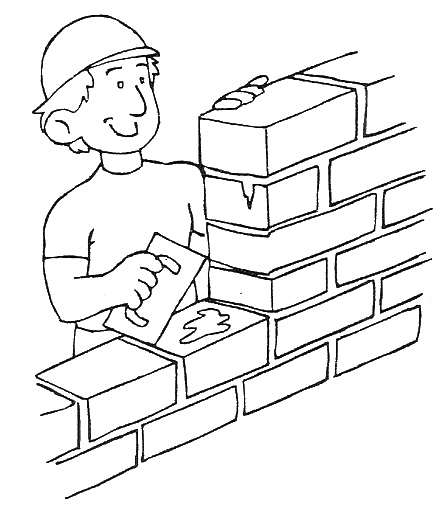
\includegraphics[scale=0.20]{gfx/bricklayer.png}
%       \end{figure}
%     %}
%   \end{minipage}
%   \hfill
%   \begin{minipage}[t]{0.45\linewidth}
%     %\onslide<2-2>{
%       \begin{figure}
%         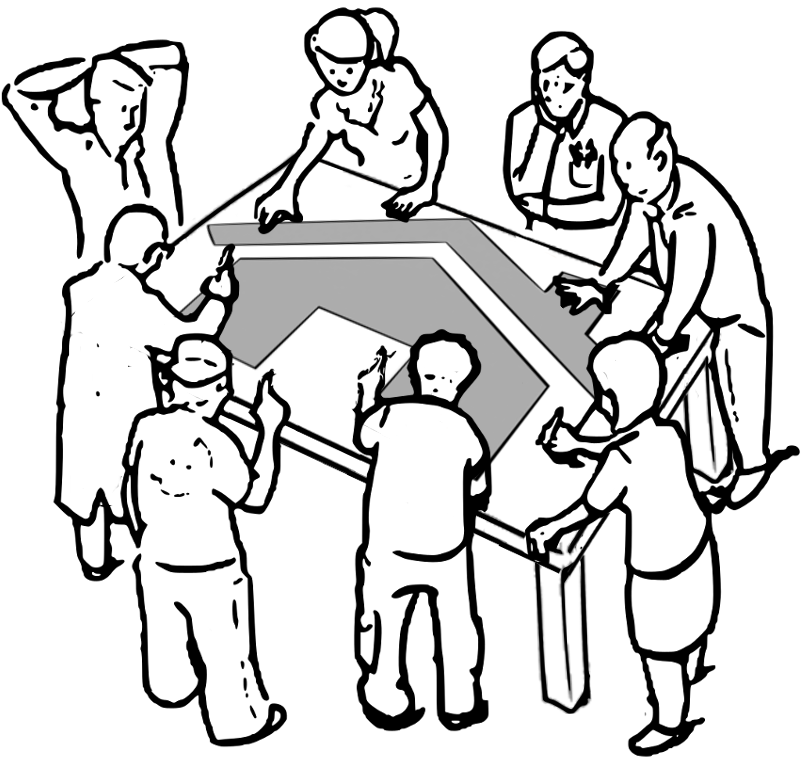
\includegraphics[scale=0.20]{gfx/introlol2.png}
%       \end{figure}
%     %}    
%   \end{minipage}
% \end{frame}
\endgroup
\section*{Introduction}
\begin{frame}{Contexte}
  \begin{small}
    \begin{quote}
      Toute information utilisée pour caractériser une entité. 
      %Une entité est une personne, un lieu, ou un objet. 
    \end{quote}
  \end{small}
\vfill

  \begin{minipage}{.48\linewidth}
\begin{coloredbox}[black]{Dimensions de contexte}
    %Dimensions de contexte:
    %\begin{itemize}
     Monde physique (état matériel). %localisation géographique
\vfill
     Monde logiciel (agenda).
\vfill
     L'utilisateur (mesures \\physiologiques).
\vfill
     Activités de l'utilisateur (ouverture de porte).
    %\end{itemize}
\end{coloredbox}
  \end{minipage}
  \hfill
  \begin{minipage}{.48\linewidth}
\begin{coloredbox}[black]{ Services \textbf{sensibles au contexte}}
    %Services \textbf{sensibles au contexte}: 
    Utiliser le contexte. 
    \vfill 
    Interagir avec l'utilisateur.
\end{coloredbox}
  \end{minipage}
\end{frame}


\begin{frame}{Sensibilité au contexte pour supporter l'autonomie domiciliaire}
  Services sensibles au contexte définis par des {\bf experts du domaine}:
  \vfill
  \begin{minipage}{.3\linewidth}
\onslide<2->{
    \begin{coloredbox}[black]{Préparer le déjeuner}
      Allumer le four.
      \\
      Ouvrir le frigidaire.
    \end{coloredbox}
}
  \end{minipage}
  \hfill
  \begin{minipage}{.3\linewidth}
\onslide<3->{
    \begin{coloredbox}[black]{Lever}
      Présence dans la chambre.
      \\
      Présence dans la cuisine.
    \end{coloredbox}
}
  \end{minipage}
  \hfill
  \begin{minipage}{.3\linewidth}
\onslide<4->{
    \begin{coloredbox}[black]{Porte entrée ouverte non surveillée}
      Ouvrir la porte d'entrée.
      \\
      Absence dans \\l'entrée.
    \end{coloredbox}
}
  \end{minipage}
  \vfill
% \onslide<5->{
%   Domaine applicatif idéal, mais il y a un certain nombre de défis.
% }
\end{frame}

\begin{frame}{Défis de l'autonomie domiciliaire}
\vspace*{-6.3mm}
\begin{minipage}{.4\linewidth}
\small
Fiabilité de la détection du contexte. 
\\
Multiples axes de variation 
\begin{scriptsize}
(Utilisateurs, domiciles, intervenants).
\end{scriptsize}

Dynamicité.
\end{minipage}
\hfill
\begin{minipage}{.5\linewidth}
    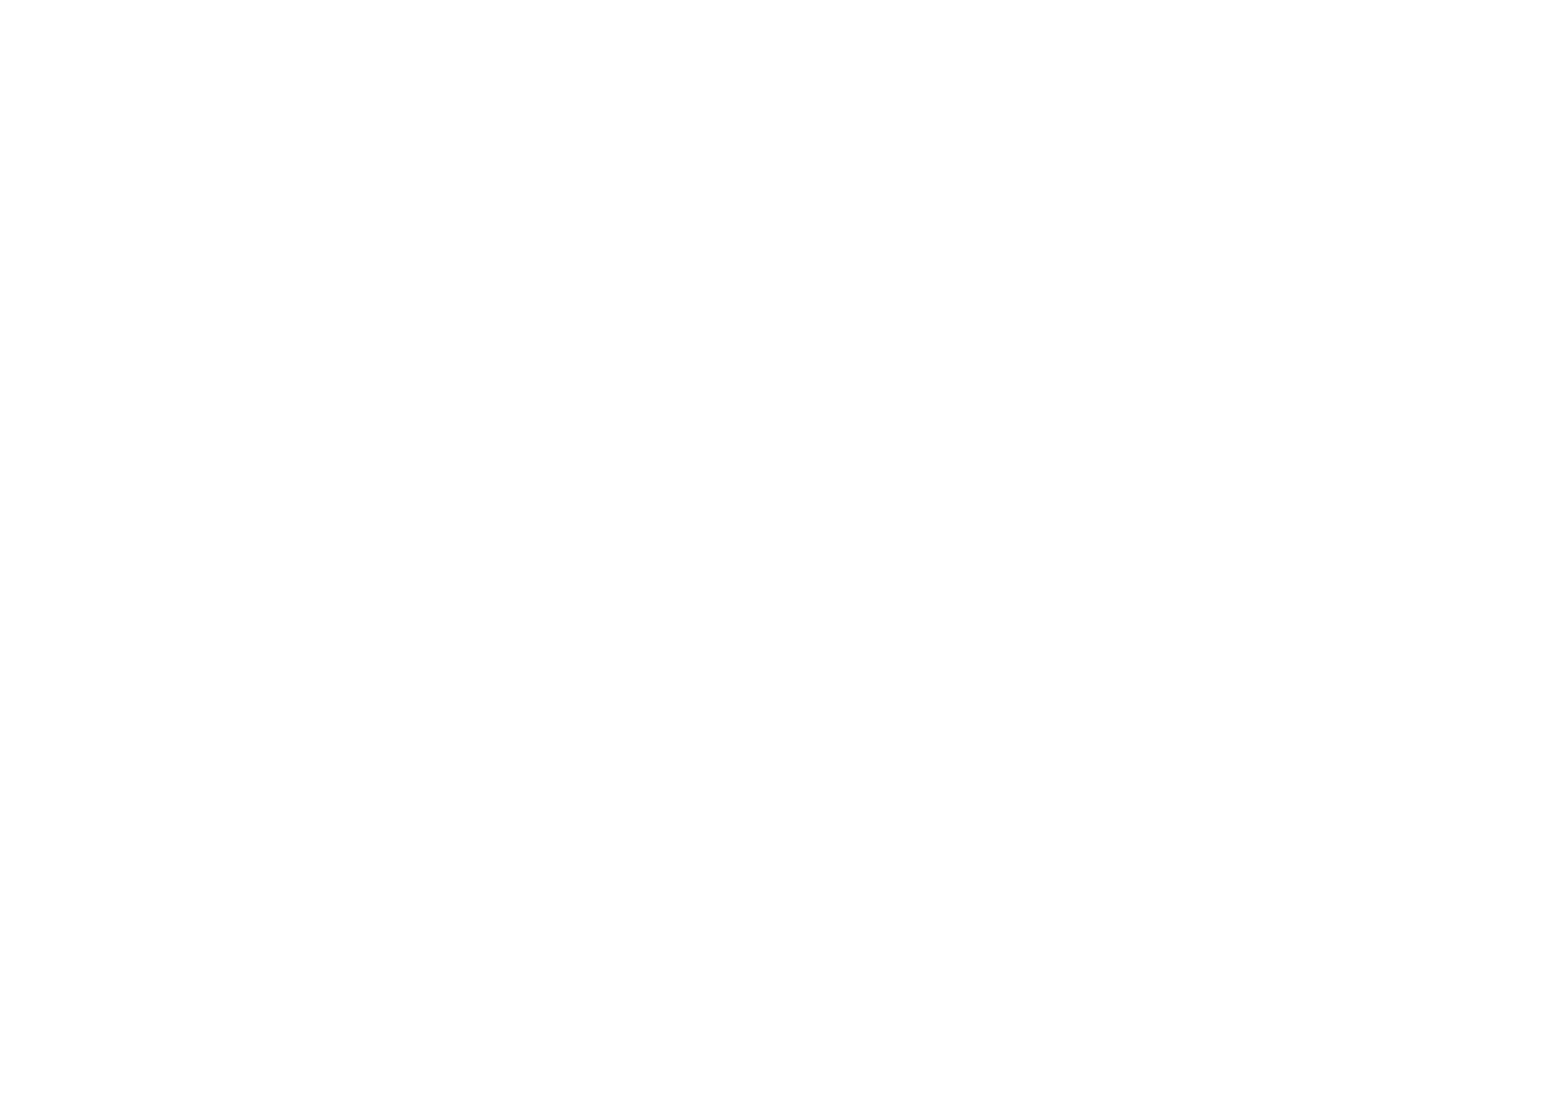
\includegraphics[scale=0.1]{axe_variation_nill.png}
\end{minipage}
\vfill
% \onslide<2->{
%   \begin{coloredbox}[red]{Problématique}
% \centering
%    Comment couvrir les besoins des services sensibles au contexte?
%   \end{coloredbox}
% }
\end{frame}

\begin{frame}{Défis de l'autonomie domiciliaire}
  \addtocounter{framenumber}{-1}
\vspace*{-6.3mm}
\begin{minipage}{.4\linewidth}
\small
Fiabilité de la détection du contexte. 
\\
Multiples axes de variation 
\begin{scriptsize}
(Utilisateurs, domiciles, intervenants).
\end{scriptsize}

Dynamicité.
\end{minipage}
\hfill
\begin{minipage}{.5\linewidth}
    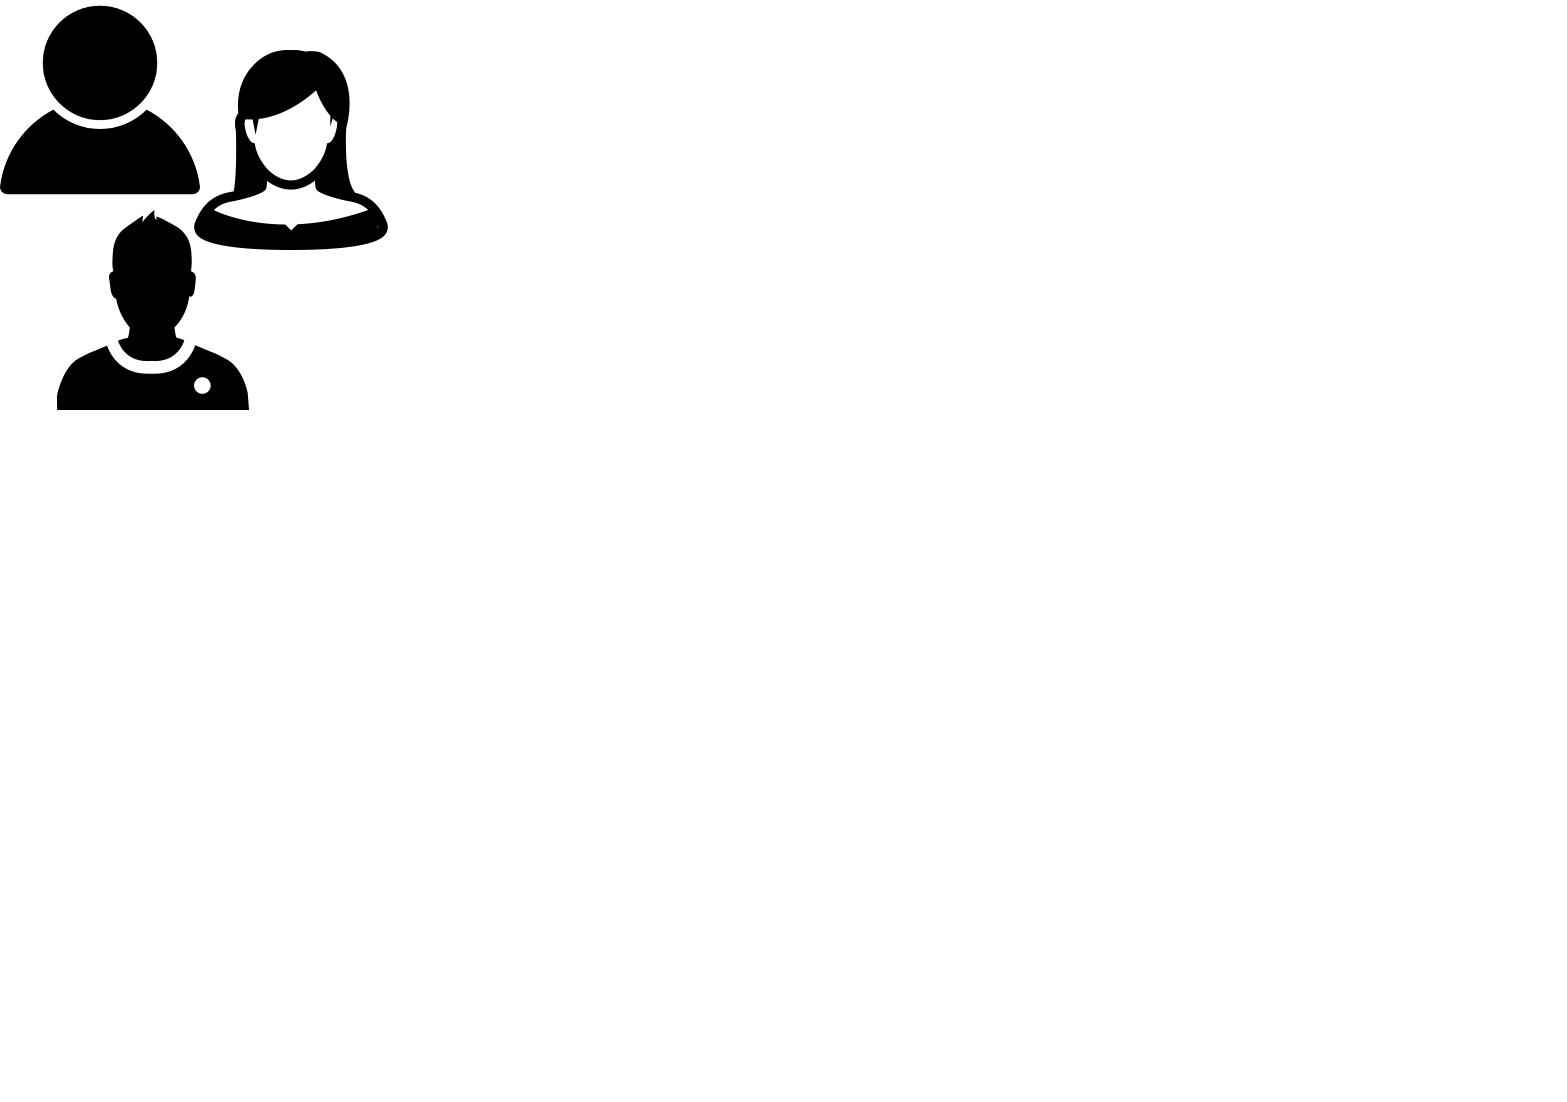
\includegraphics[scale=0.1]{axe_variation_1.png}
\end{minipage}
\vfill
% \onslide<2->{
%   \begin{coloredbox}[red]{Problématique}
% \centering
%    Comment couvrir les besoins des services sensibles au contexte?
%   \end{coloredbox}
% }
\end{frame}

\begin{frame}{Défis de l'autonomie domiciliaire}
  \addtocounter{framenumber}{-1}
\vspace*{-6.3mm}
\begin{minipage}{.4\linewidth}
\small
Fiabilité de la détection du contexte. 
\\
Multiples axes de variation 
\begin{scriptsize}
(Utilisateurs, domiciles, intervenants).
\end{scriptsize}

Dynamicité.
\end{minipage}
\hfill
\begin{minipage}{.5\linewidth}
    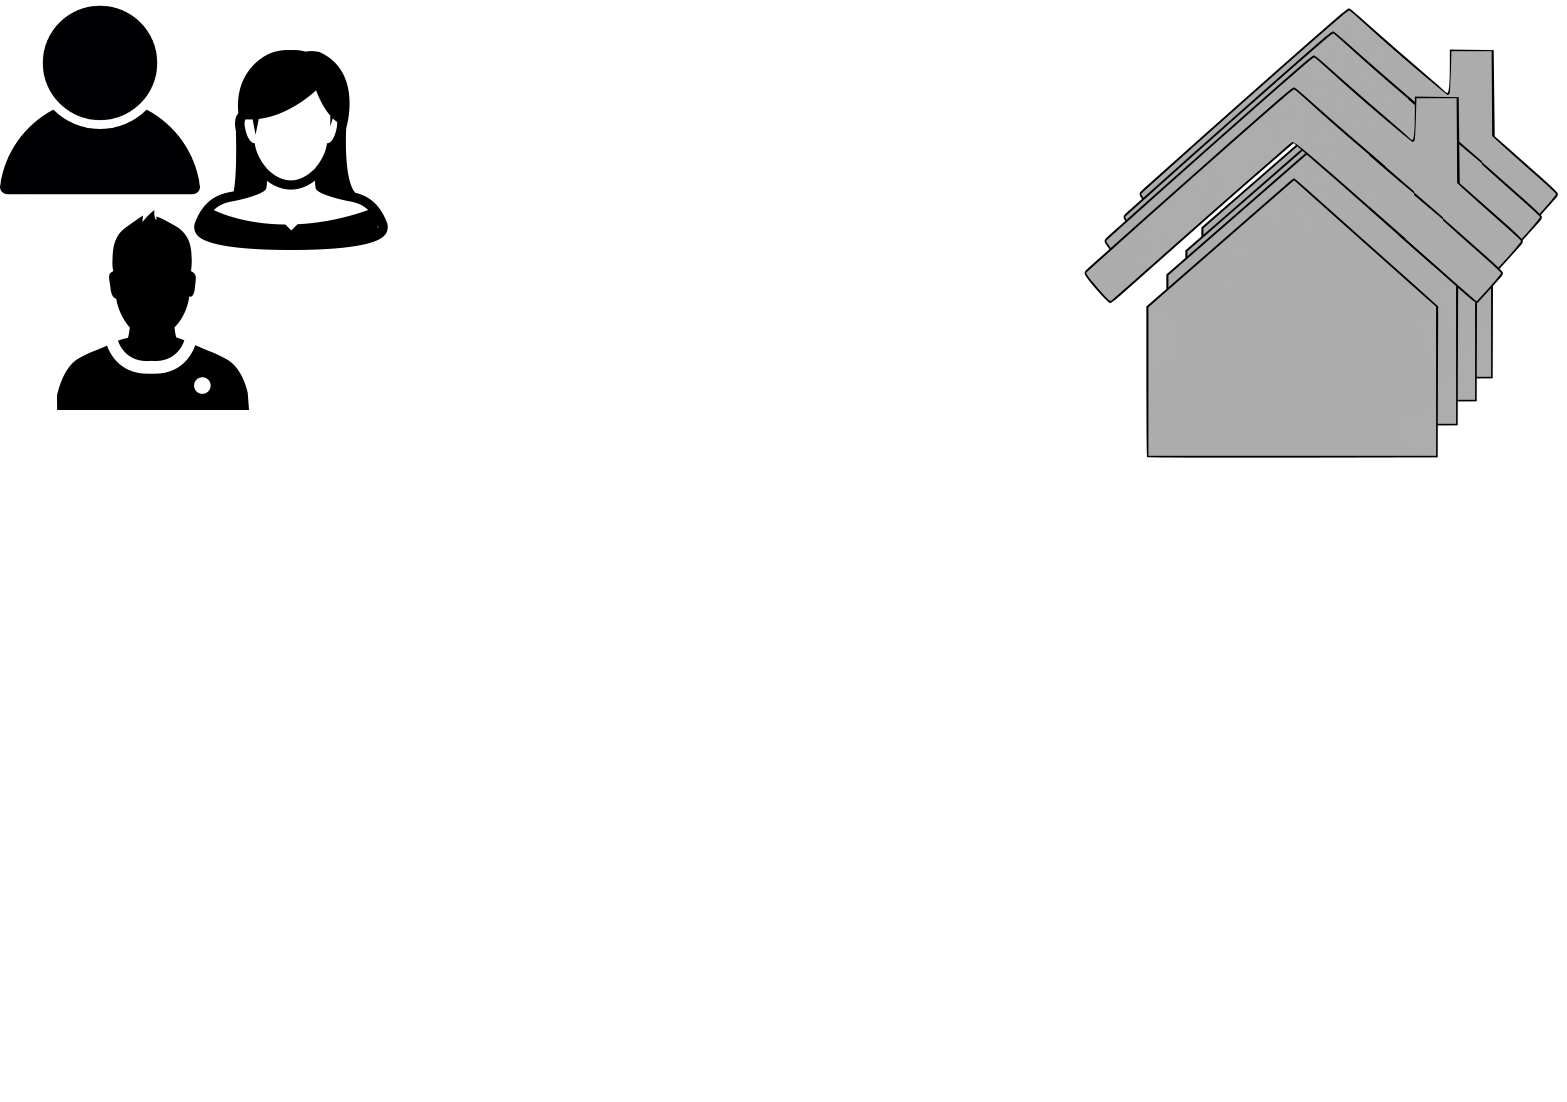
\includegraphics[scale=0.1]{axe_variation_2.png}
\end{minipage}
\vfill
% \onslide<2->{
%   \begin{coloredbox}[red]{Problématique}
% \centering
%    Comment couvrir les besoins des services sensibles au contexte?
%   \end{coloredbox}
% }
\end{frame}

\begin{frame}{Défis de l'autonomie domiciliaire}
  \addtocounter{framenumber}{-1}
\vspace*{-6.3mm}
\begin{minipage}{.4\linewidth}
\small
Fiabilité de la détection du contexte. 
\\
Multiples axes de variation 
\begin{scriptsize}
(Utilisateurs, domiciles, intervenants).
\end{scriptsize}

Dynamicité.
\end{minipage}
\hfill
\begin{minipage}{.5\linewidth}
    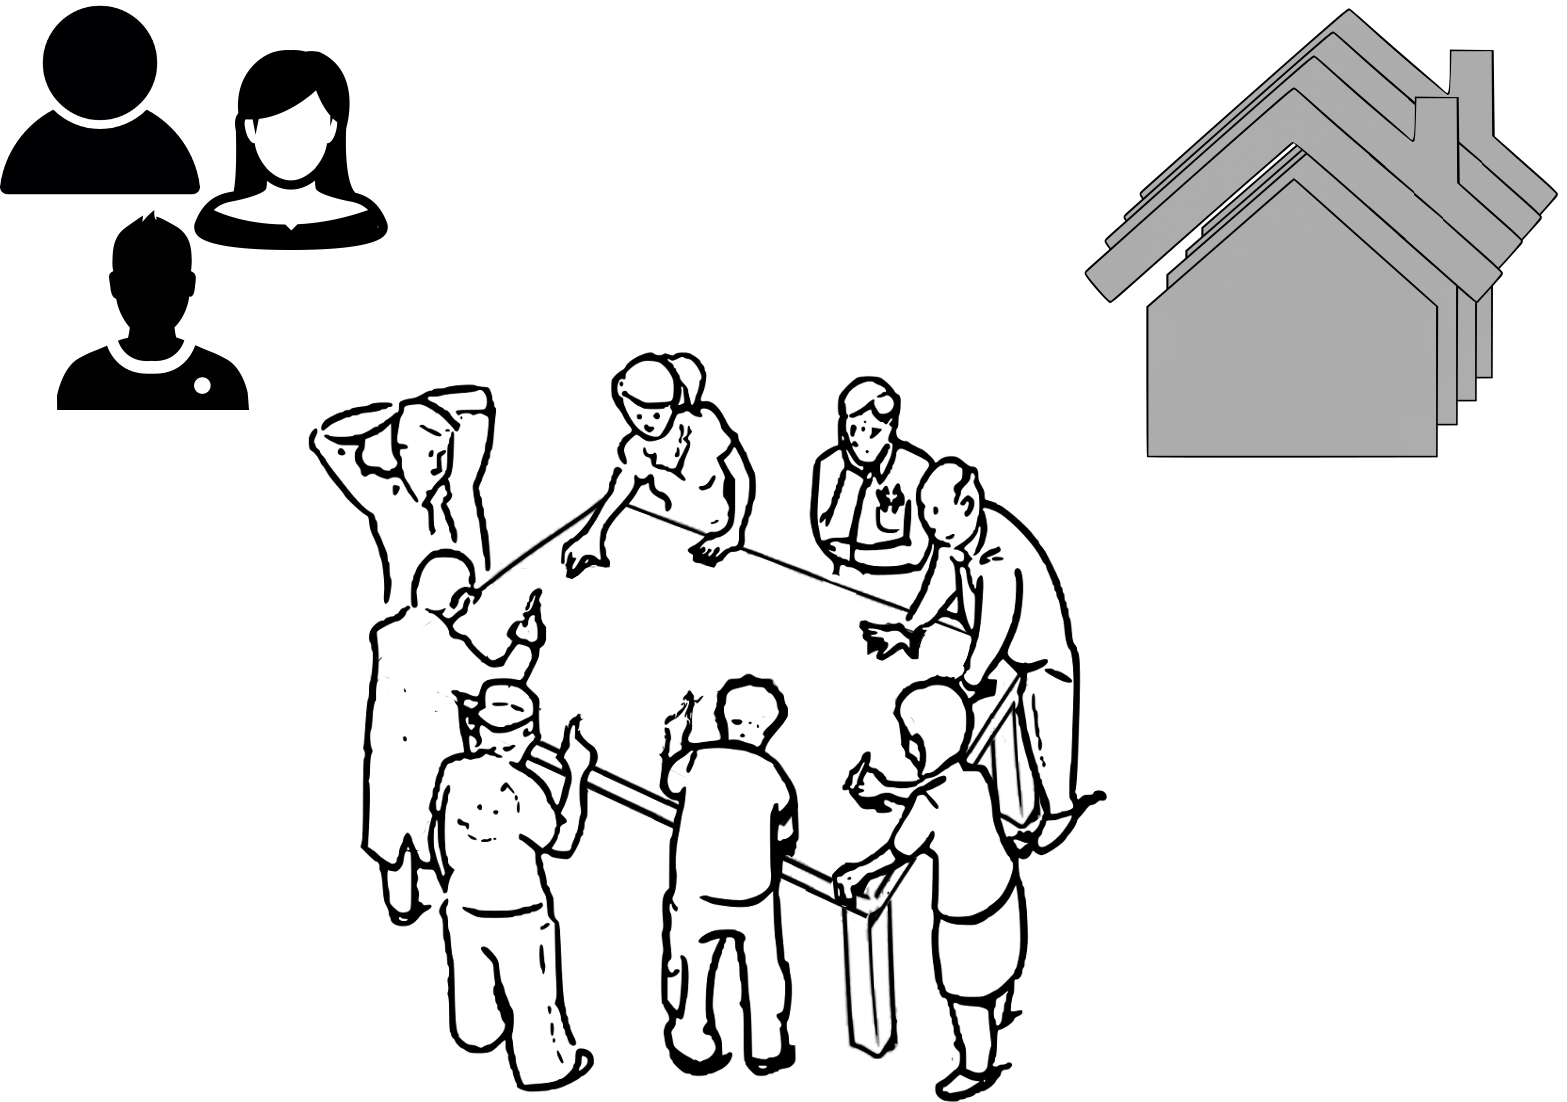
\includegraphics[scale=0.1]{axe_variation_int.png}
\end{minipage}
\vfill
% \onslide<2->{
%   \begin{coloredbox}[red]{Problématique}
% \centering
%    Comment couvrir les besoins des services sensibles au contexte?
%   \end{coloredbox}
% }
\end{frame}

\begin{frame}{Défis de l'autonomie domiciliaire}
  \addtocounter{framenumber}{-1}
\begin{minipage}{.4\linewidth}
\small
Fiabilité de la détection du contexte. 
\\
Multiples axes de variation 
\begin{scriptsize}
(Utilisateurs, domiciles, intervenants).
\end{scriptsize}

Dynamicité.
\end{minipage}
\hfill
\begin{minipage}{.5\linewidth}
    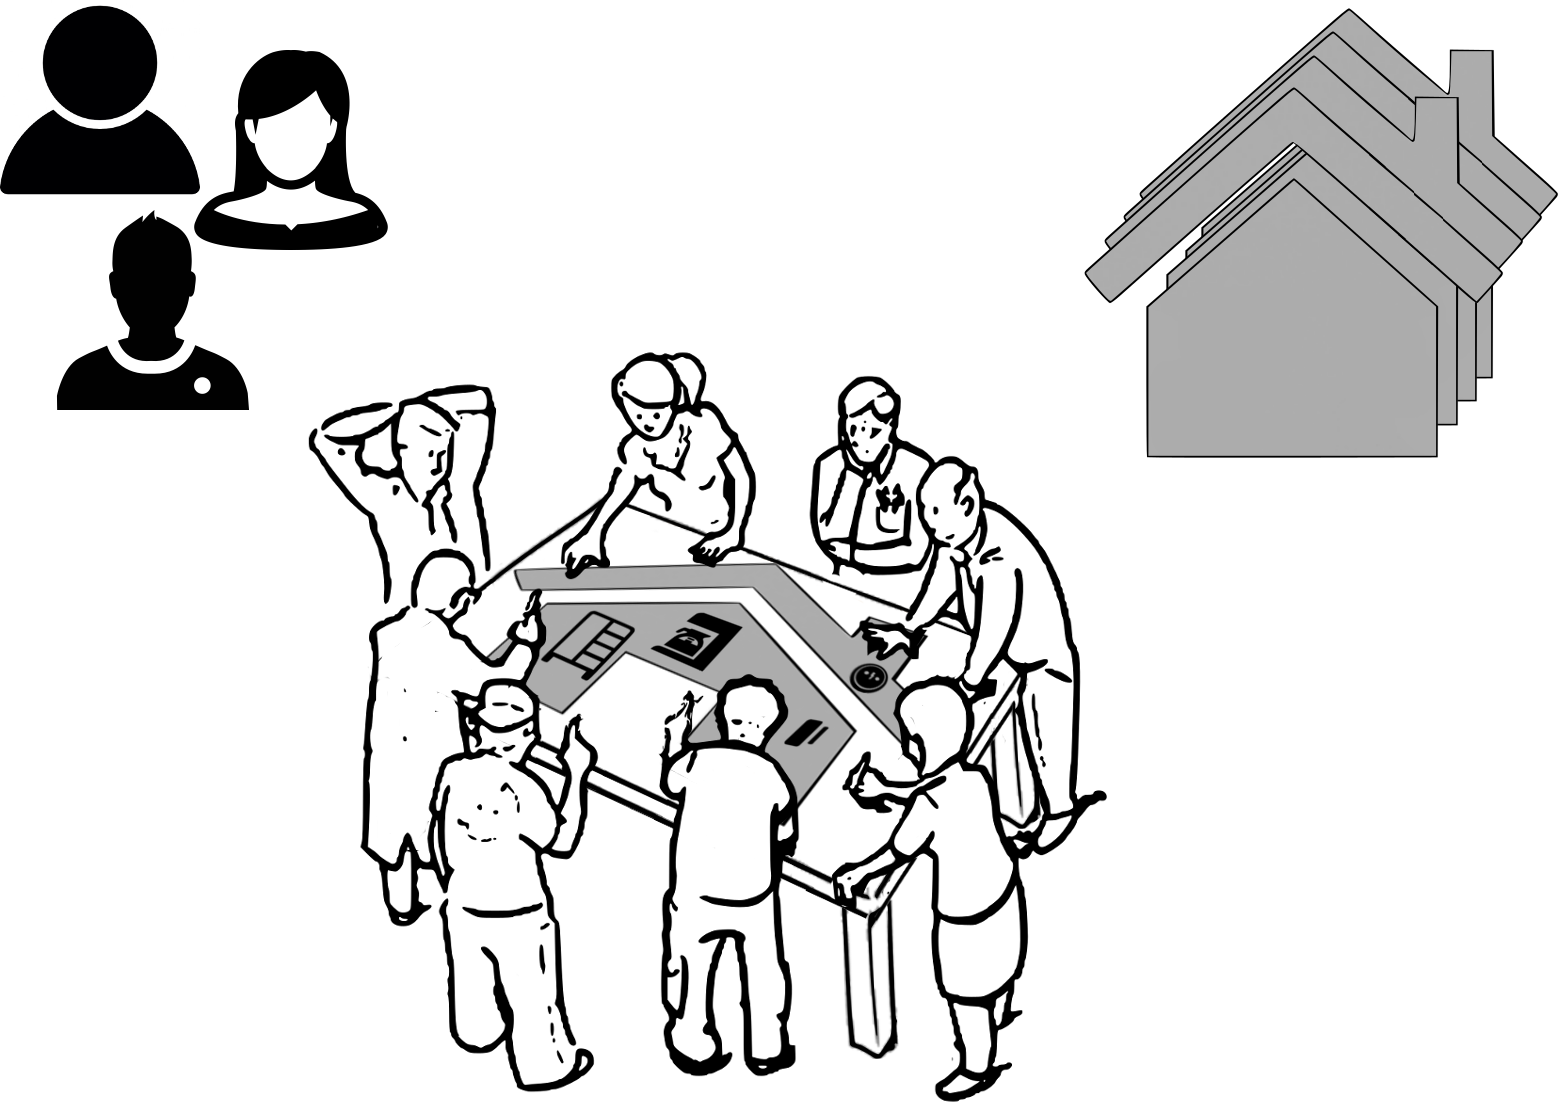
\includegraphics[scale=0.1]{axe_variation_3.png}
\end{minipage}
%\vfill
% \onslide<2->{
%
  \begin{coloredbox}[red]{Problématique}
\centering
   Comment couvrir les besoins des services sensibles au contexte?
  \end{coloredbox}
% }
\end{frame}

% \begin{frame}{Défis de l'autonomie domiciliaire}
% \begin{minipage}{.4\linewidth}
% \onslide<1->{
% \small
%   %\begin{itemize}
% %  \item 
% Fiabilité de la détection du contexte. %liée à l'acceptabilité.
% %  \item 
% \\
% Multiples axes de variation 
% \begin{scriptsize}
% (Utilisateurs, domiciles, intervenants).
% \end{scriptsize}
%   %\item Différents intervenants.% pour définir les services (assistance, maintenance).
%   %\item Différents services.% et objectifs de services (Surveillance de petit-déjeuner, batterie de capteurs, surveillance du réseau).
%   %\item Différentes configurations de domiciles.
%   %\item 

% Dynamicité.
%   %\end{itemize}
% } 
% \end{minipage}
% \hfill
% \begin{minipage}{.5\linewidth}
% \onslide<2->{
%     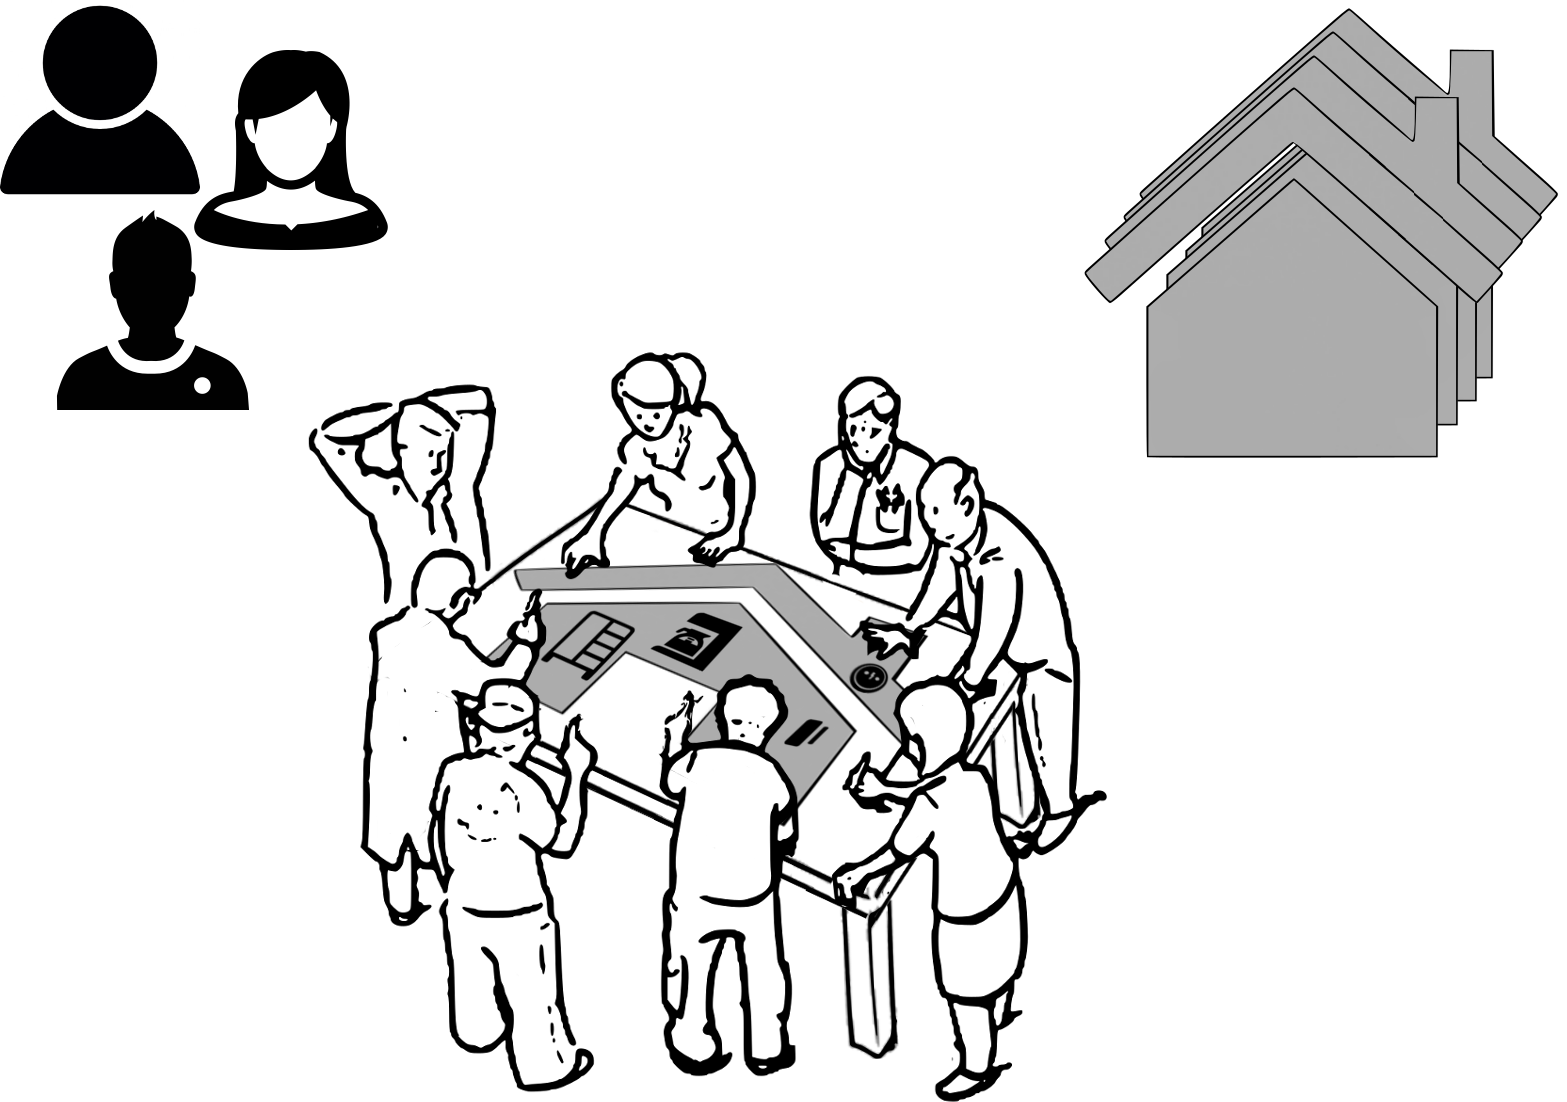
\includegraphics[scale=0.1]{axe_variation0.png}
% }
% \end{minipage}
% \vfill
% \onslide<2->{
%   \begin{coloredbox}[red]{Problématique}
% \centering
%    Comment couvrir les besoins des services sensibles au contexte?
%   \end{coloredbox}
% }
% \end{frame}

% \begin{frame}{Problématique}
%   \begin{coloredbox}[red]{Comment couvrir les besoins de l'autonomie domiciliaire des personnes âgées ?}
%     \begin{itemize}
%     \item Fiabilité de la sensibilité au contexte.
%     \item Différents intervenants.
%     \item Réactivité.
%     \item Passage à l'échelle. %\notespeech{(many homes, many users, many users needs)}.
%     \end{itemize}
%   \end{coloredbox}
% \end{frame}

\begin{frame}{État de l'art}
  Fiabilité de la sensibilité au contexte~:\\
  \begin{itemize}
  \item Simulation de contexte~\cite{bruno2009diasim}.
    \begin{itemize}[label=--,font=\LARGE \color{black}]
    \item Limité aux couches applicatives.
    \end{itemize}
  \item Placement de capteurs~\cite{hong2013toward,murao2013evaluation,beckmann2004some}.
    \begin{itemize}[label=--,font=\LARGE \color{black}]
    \item Intrusifs (caméra, capteurs portés).
    \item Usage en laboratoire (Gants RFID).
    %\item Principes théoriques sans méthodes systématiques.
    \end{itemize}
  \end{itemize}

\end{frame}
\begin{frame}{État de l'art}
  Intervenants~:
  \begin{itemize}
  \item Programmation par les utilisateurs~\cite{resnick2009scratch,coutaz2016first,criel2011deconstructing}.
    \begin{itemize}[label=--,font=\LARGE \color{black}]
    \item Expressivité limitée.
    \item Généralistes.
    \end{itemize}
  \item Services d'assistance domiciliaire~\cite{hoque2015holmes,lee2015sensor,baecker2014technology}.
    \begin{itemize}[label=--,font=\LARGE \color{black}]
    \item Approches en silo.
    \end{itemize}
  \end{itemize}
  %Scaling-up~:\\

  Réactivité~:
  \begin{itemize}
  \item Approches de traitement événementiel~\cite{cugola2012processing}.
    \begin{itemize}[label=--,font=\LARGE \color{black}]
    \item Complexe à mettre en {\oe}uvre.
    \end{itemize}
  \end{itemize}
\end{frame}

\begin{frame}{Thèse~: Unifier l'expression des contextes.}
%\begin{center}
 % \begin{itemize}
    \onslide<1->{
%    \item 
\hspace{50mm}
Modèle d'infrastructure% pour la fiabilité de la sensibilité au contexte.
      \begin{itemize}[label=$\rightarrow$,font=\LARGE \color{red}]
      \item \begin{center}Fiabilité.\end{center}
      \end{itemize}
    }
\vfill
    \onslide<2->{
%    \item 
\hspace{50mm}
Langage dédié.
\hspace{50mm}
      \begin{itemize}[label=$\rightarrow$,font=\LARGE \color{red}]
      %\item Passage à l'échelle.
      \item \begin{center}Axes de variation.\end{center}
      \end{itemize}
    }
\vfill
    \onslide<3->{
%    \item 
\hspace{50mm}
Paradigme événementiel.
\hspace{50mm}
      \begin{itemize}[label=$\rightarrow$,font=\LARGE \color{red}]
      \item \begin{center}Dynamicité.\end{center}
      \end{itemize}
    }

  %\end{itemize}
%\end{center}
\end{frame}

% \begin{frame}{Thèse~: Unifier l'expression des contextes.}
% \begin{minipage}{.4\linewidth}
% \begin{coloredbox}[red]{}
%   \begin{itemize}
%   \item Fiabilité.
%   \item Passage à l'échelle, différents intervenants.
%   \item Temps réel.
%   \end{itemize}
% \end{coloredbox}
% \end{minipage}
% \hfill
% \begin{minipage}{.55\linewidth}
% \begin{coloredbox}[blue]{}
%   \begin{itemize}
%   \item Modèle d'infrastructure pour la fiabilité de la sensibilité au contexte.
%   \item Approche unifiée avec un langage dédié.
%   \item Approche implantée utilisant un paradigme événementiel
%   \end{itemize}
% \end{coloredbox}
% \end{minipage}
% Domicile sensible au contexte fiable\\
% Approche dirigée par les évènements et unifiée\\
% \vfill
% Approche unifiée avec un langage dédié\\
% Approche implantée utilisant un paradigme événementiel\\
% Validation\\
% Modèle d'infrastructure pour la fiabilité de la sensibilité au contexte


% Need of a reliable context-awareness home \\
% to provide an event-driven and unified approach\\
% \vfill
% unified approach with a domain specific language\\
% implemented approach using event-driven paradigm\\
% validation\\
% infrastructure model to ensure context-awareness reliability

%\end{frame}


\begingroup
\setbeamertemplate{footline}{} 
\begin{frame}{Sommaire}
\addtocounter{framenumber}{-1}
  \setbeamertemplate{section in toc}[sections numbered]
  \tableofcontents[hideallsubsections]
\end{frame}
\endgroup
% \begin{frame}
%  \frametitle{Plan}
%   \tableofcontents
%   %\tableofcontents[hideothersubsections]
% \end{frame}

%\endgroup


%\section{Related work}
%\section{Fiabilité de la sensibilité au contexte}

\begin{frame}{Rendre explicite le modèle implicite}
  \begin{minipage}{0.3\linewidth}
      \begin{figure}
        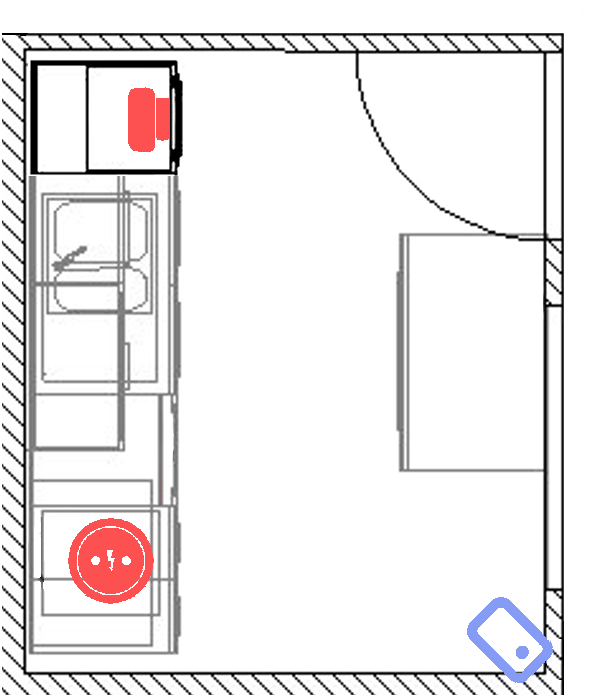
\includegraphics[scale=0.15]{use_case1.png}
      \end{figure}
    \end{minipage}
  \hfill
  \begin{minipage}{0.65\linewidth}
    %\vspace*{-25.9mm}
    \begin{coloredbox}[black]{Dépendance de présence}
      \footnotesize
      Chaque interaction (sauf présence) doit être recouverte par une interaction de présence.
      \small
      \begin{displaymath}
        \begin{array}{c}
        ~\\
        ~
        \end{array}
      \end{displaymath}
    \end{coloredbox}
    \begin{coloredbox}[black]{Non ubiquité}
      \footnotesize
      Une présence ne peut pas être simultanément détectée dans deux endroits différents.
      \small
      \begin{displaymath}
        \begin{array}{c}
         ~\\ 
         ~
        \end{array}
      \end{displaymath}
    \end{coloredbox}
  \end{minipage}
\end{frame}

\begin{frame}{Rendre explicite le modèle implicite}
  \addtocounter{framenumber}{-1}
  \begin{minipage}{0.3\linewidth}
      \begin{figure}
        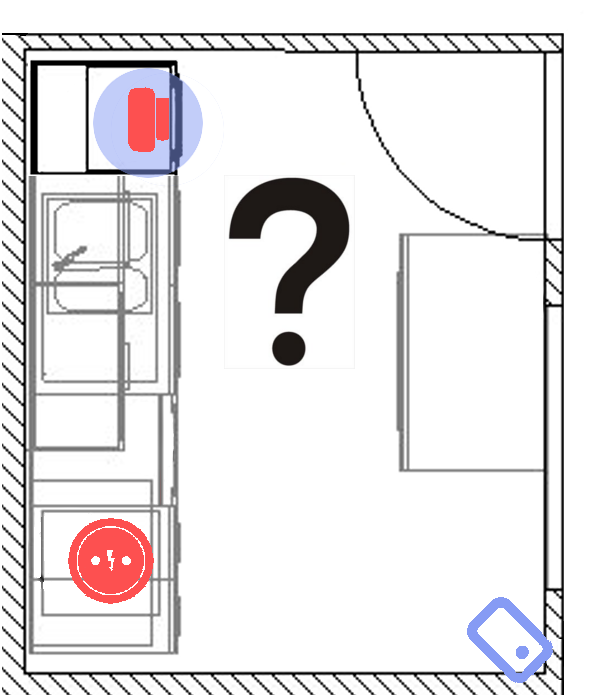
\includegraphics[scale=0.15]{use_case_issue_1.png}
      \end{figure}
    \end{minipage}
  \hfill
  \begin{minipage}{0.65\linewidth}
    %\vspace*{-25.9mm}
    \begin{coloredbox}[black]{Dépendance de présence}
      \footnotesize
      Chaque interaction (sauf présence) doit être recouverte par une interaction de présence.
      \small
      \begin{displaymath}
        \begin{array}{c}
        ~\\
        ~
        \end{array}
      \end{displaymath}
    \end{coloredbox}
    \begin{coloredbox}[black]{Non ubiquité}
      \footnotesize
      Une présence ne peut pas être simultanément détectée dans deux endroits différents.
      \small
      \begin{displaymath}
        \begin{array}{c}
         ~\\ 
         ~
        \end{array}
      \end{displaymath}
    \end{coloredbox}
  \end{minipage}
\end{frame}

\begin{frame}{Rendre explicite le modèle implicite}
  \addtocounter{framenumber}{-1}
  \begin{minipage}{0.3\linewidth}
      \begin{figure}
        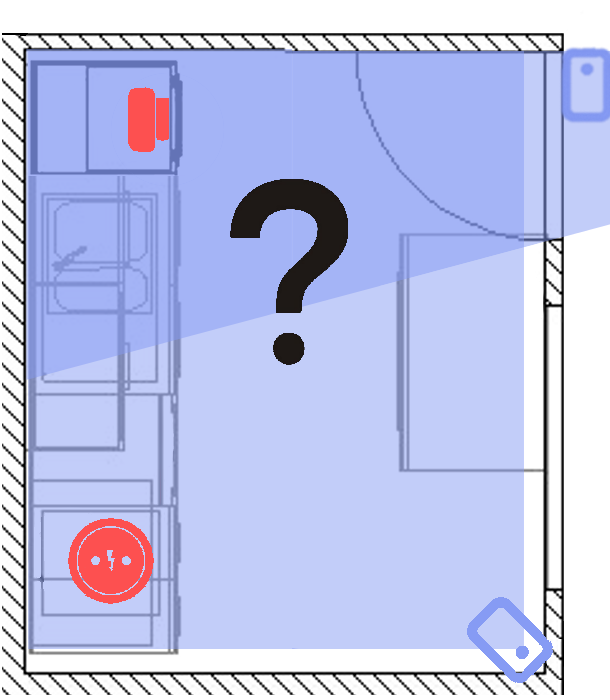
\includegraphics[scale=0.15]{use_case_issue_2.png}
      \end{figure}
    \end{minipage}
  \hfill
  \begin{minipage}{0.65\linewidth}
    %\vspace*{-25.9mm}
    \begin{coloredbox}[black]{Dépendance de présence}
      \footnotesize
      Chaque interaction (sauf présence) doit être recouverte par une interaction de présence.
      \small
      \begin{displaymath}
        \begin{array}{c}
        ~\\
        ~
        \end{array}
      \end{displaymath}
    \end{coloredbox}
    \begin{coloredbox}[black]{Non ubiquité}
      \footnotesize
      Une présence ne peut pas être simultanément détectée dans deux endroits différents.
      \small
      \begin{displaymath}
        \begin{array}{c}
         ~\\ 
         ~
        \end{array}
      \end{displaymath}
    \end{coloredbox}
  \end{minipage}
\end{frame}

\begin{frame}{Rendre explicite le modèle implicite~: Modèle d'infrastructure}
  \addtocounter{framenumber}{-1}
  \begin{minipage}{0.3\linewidth}
      \begin{figure}
        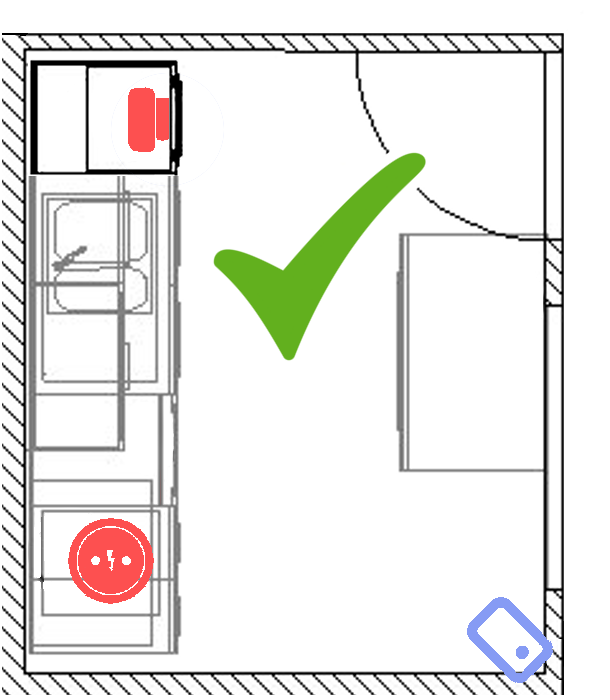
\includegraphics[scale=0.15]{use_case_final.png}
      \end{figure}
    \end{minipage}
  \hfill
  \begin{minipage}{0.65\linewidth}
    \begin{coloredbox}[black]{Dépendance de présence}
      \footnotesize
      Chaque interaction (sauf présence) doit être recouverte par une interaction de présence.
      \small
      \begin{displaymath}
        \begin{array}{c}
          \forall~<k, Kitchen, p>~\in~Log, k \neq Presence~ \Rightarrow \\
          ~~~~\exists~ <Presence, Kitchen, p'>~\in~Log,~p \subseteq p' 
        \end{array}
      \end{displaymath}
    \end{coloredbox}
    \begin{coloredbox}[black]{Non ubiquité}
      \footnotesize
      Une présence ne peut pas être simultanément détectée dans deux endroits différents.
      \small
      \begin{displaymath}
        \begin{array}{c}
          \forall~<Presence, l, p>~\in~Log \Rightarrow \\
          ~~~~\nexists~ <Presence, l', p'>~\in~Log,~l \neq l' \wedge ~p' \cap p \neq \emptyset
        \end{array}
      \end{displaymath}

    \end{coloredbox}
  \end{minipage}
\end{frame}
% **********************************************

% \begin{frame}{Rendre explicite le modèle implicite}
%   % Abstraction de roles de capteurs: {\footnotesize \( e~\in~Event = Kind \times Loc \times Period\)}

%   \begin{minipage}{0.3\linewidth}
%     \onslide<1->{
%       \begin{figure}
%         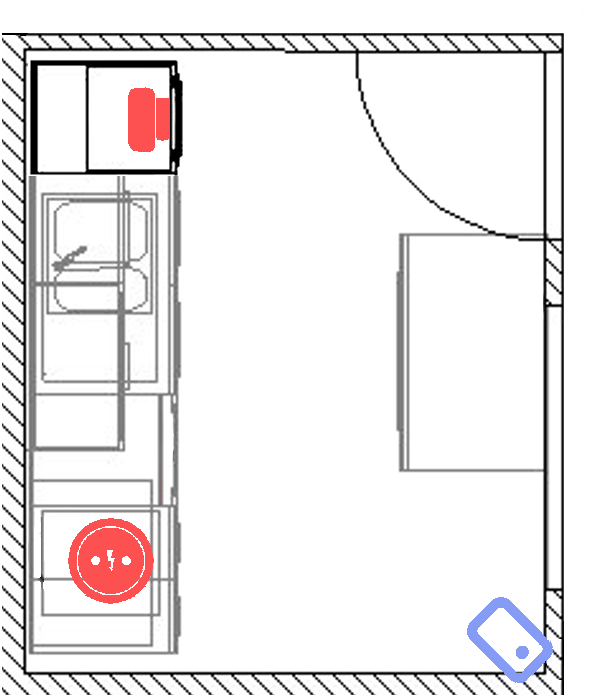
\includegraphics[scale=0.15]{use_case1.png}
%       \end{figure}
%       % \begin{footnotesize}
%       %   \begin{coloredbox}[teal]{Hypothèses}
%       %     \begin{itemize}
%       %     \item Détection de mouvement précède toute autre interaction.
%       %     \item Une présence dans une pièce ne peut pas recouvrir une présence dans une autre pièce.
%       %     \end{itemize}
%       %   \end{footnotesize}
%       }
%     \end{minipage}
%   \hfill
%   \begin{minipage}{0.65\linewidth}
%     \begin{coloredbox}[gray]{Dépendance de présence}
%       \footnotesize
% \onslide<1->{
%       Chaque interaction (sauf présence) doit être recouverte par une interaction de présence.% à la même localisation
%       % Any detected interaction (but presence) must be surrounded by a presence interaction
% }
%       \small
% \onslide<2->{
%       \begin{displaymath}
%         \begin{array}{c}
%           \forall~<k, Kitchen, p>~\in~Log, k \neq Presence~ \Rightarrow \\
%           ~~~~\exists~ <Presence, Kitchen, p'>~\in~Log,~p \subseteq p' 
%         \end{array}
%       \end{displaymath}
% }
%     \end{coloredbox}
%     %\vfill
%     \begin{coloredbox}[gray]{Non ubiquité}
%       \footnotesize
% \onslide<1->{
%       Une présence ne peut pas être simultanément détectée dans deux endroits différents.
% }
%       \small
% \onslide<3->{
%       \begin{displaymath}
%         \begin{array}{c}
%           \forall~<Presence, l, p>~\in~Log \Rightarrow \\
%           ~~~~\nexists~ <Presence, l', p'>~\in~Log,~l \neq l' \wedge ~p' \cap p \neq \emptyset
%         \end{array}
%       \end{displaymath}
% }
%     \end{coloredbox}
%   \end{minipage}
 
% \end{frame}
% **********************************************
% **********************************************
\begin{frame}[fragile]{Validation avec le projet pilote de Domassist}
%\begin{minipage}[t]{0.45\linewidth}
\begin{coloredbox}[black]{Assistance domiciliaire pour personnes âgées}
 % Aims: Aging in place\linebreak
  %\vfill
\footnotesize
  Services définis par des ergothérapeutes, psychologues, experts en vieillissement.\\%\linebreak
  %Activities defined by experts in occupational therapy and psychology and aging\linebreak
  %\vfill
  
  \begin{itemize}
  \item Applications de surveillance des activités du quotidien.
  \item Applications de sécurité du domicile et de l'utilisateur.
  \end{itemize}
  %\vfill
  Étude conduite avec 24 participants vivant seuls pendant 9 mois.
  %Field study: conducted with 24 older participants for a period of 9 months
\end{coloredbox}
\vfill
%\end{minipage}
%\hfill
%\begin{minipage}[t]{0.45\linewidth}
   \begin{table}[!h]
    \begin{scriptsize}
      \begin{tabular}{| c | c |} \hline
        {\bf Name} & {\bf Rule} \\ \hline \hline
        Dépendance de présence & 
$\forall~<i, l, p>~\in~Log, i \neq Presence~ \Rightarrow$\\
        &$~~~\exists~ <Presence, l, p'>~\in~Log,~p \subseteq p'$
%\end{displaymath} 
\\ \hline
        Porte restée ouverte & $\forall~<Opening, l, p>~\in~Log \Rightarrow  \# p < MAX$  \\ \hline
        Non ubiquité & $\forall~<Presence, l, p>~\in~Log \Rightarrow$ \\
     &$~~~~\nexists~ <Presence, l', p'>~\in~Log,~l \neq l' \wedge ~p' \cap p \neq \emptyset$ \\ \hline
         Taux de déclenchement & $\forall~<k, l, p>~\in~Log \Rightarrow$ \\
     &$~~~~~\# (p - Prev(<k, l, p>)) < MAX$ \\ \hline
      \end{tabular}
    \end{scriptsize}
    \vspace{5mm}
    \label{scenario-fig}
    %\caption{Example de scénarios de services d'assistance.}
  \end{table}
%\end{minipage}
\end{frame}
% **********************************************
\begin{frame}{Fiabilité~: Résultats }
  \begin{minipage}[h]{0.45\linewidth}
    \begin{coloredbox}[black]{
        Non-conformités permanentes~:%}
      }
      \onslide<2->{
        %\begin{figure}
          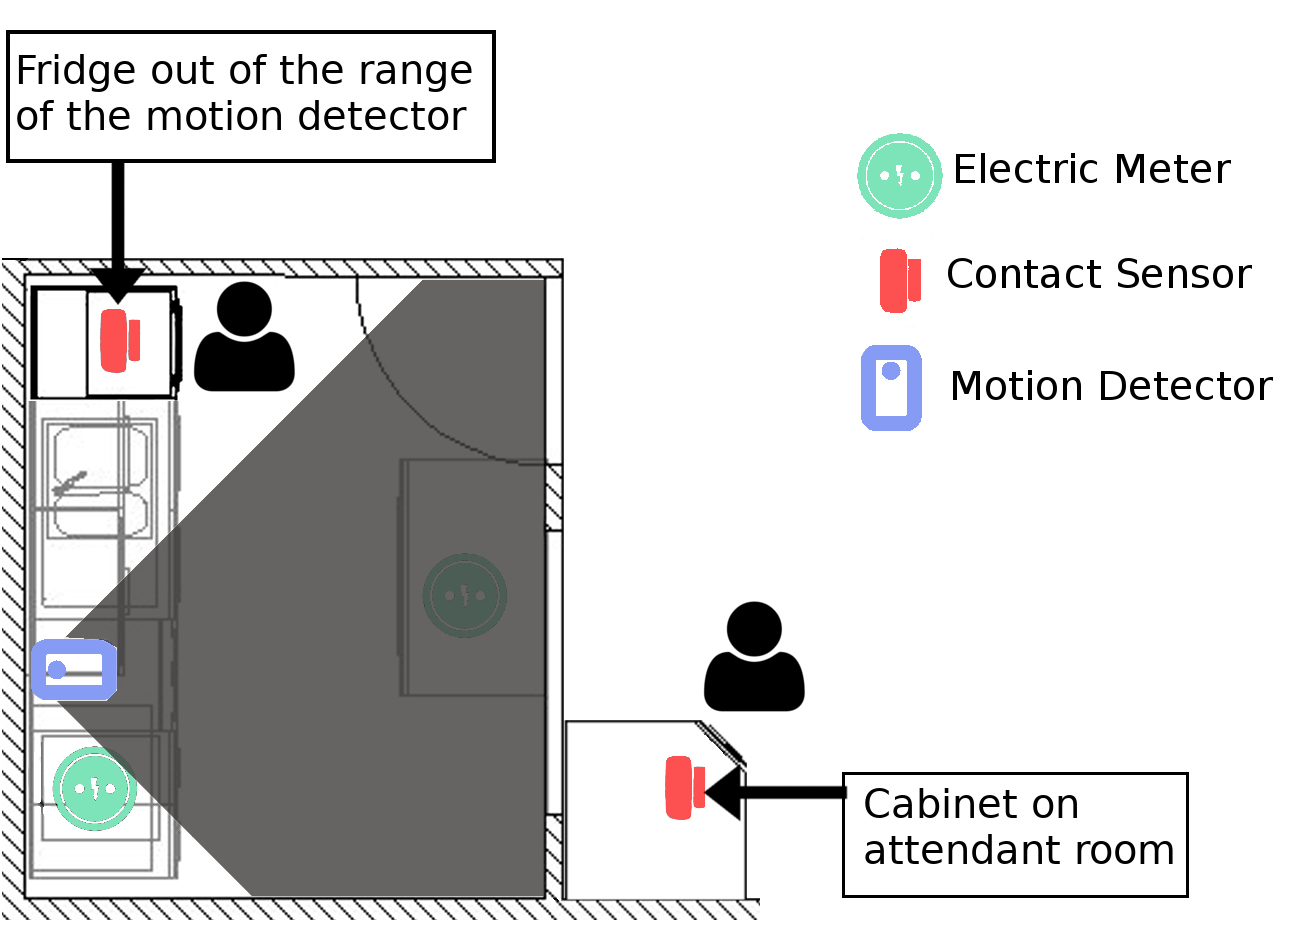
\includegraphics[scale=0.125]{nconf3.png}
          %\label{fig:map}
        %\end{figure}
        \begin{itemize}[label=$\rightarrow$,font=\LARGE \color{black}]
        \item Adapter le modèle.
        \item Repositionner le capteur. 
        \end{itemize}
      }
    \end{coloredbox}
    
  \end{minipage}
  \hfill
  \begin{minipage}[h]{0.45\linewidth}
    \begin{coloredbox}[black]{
        Non-conformités émergentes~: }
      \begin{small}
\onslide<3->{
        \begin{itemize}
        %\item \textbf{Porte restée ouverte~:} \\Chute du capteur de contact.
        \item Chute du capteur de contact.
        %\item \textbf{Dépendance de présence~:}\\Capteur de mouvement défaillant.
        \item Capteur de mouvement défaillant.
%        \item \textbf{Non ubiquité~:}\\Latence des detecteurs de mouvements.

        \end{itemize}
        \vfill
        \begin{itemize}[label=$\rightarrow$,font=\LARGE \color{black}]
        \item Intervention d'un technicien.
        \end{itemize}
}
      \end{small}
    \end{coloredbox}
  \end{minipage}
\end{frame}
% **********************************************
\begin{frame}{Synthèse~: Assurer la fiabilité du contexte\\
Modèle d'infrastructure explicite sous forme de règles~\cite{carteron2016improving}
}
\begin{coloredbox}[checked]{Conformité d'une installation avec un modèle}
%Conformité d'une installation avec un modèle:
  \begin{itemize}%[<+->]
  \item Certifie l'installation.
  \item Guide l'installation.
  \item Application certifiée pour un modèle/installation.
  \end{itemize}
\end{coloredbox}
\vfill
\begin{coloredbox}[checked]{Vérification continue}
%Vérification continue:  
  \begin{itemize}
  \item Détection des pannes.
  \item Aide au diagnostic.
  \end{itemize}
\end{coloredbox}
\vfill

%~\cite{carteron2016improving}
\end{frame}
% **********************************************

% **********************************************
\section{Analyse de domaine}
% \begin{frame}{Analyse de domaine}
% À partir de l'activité:
% \begin{itemize}
% \item Étude de scénarios.
% \item Définition de la sensibilité au contexte.
% \end{itemize}
% \end{frame}
\begin{frame}{Expérimentation écologique à large échelle}
\onslide<1->{
\begin{coloredbox}[black]{Domassist}
Déploiement~:
  \begin{itemize}
  \item 12 mois.
  \item 129 personnes vivant seules.
  \item 82 ans en moyenne.
  \end{itemize}

%% Avantage d'un déploiement large échelle:
 %  \begin{itemize}
 %  \item Seniors avec troubles cognitifs implique un éventail de services.
 %  \item Étude à long terme implique de la réactivité de la maintenance.
 %  \item Déploiement large échelle nécessite des services d'administration.
 %  %\item Les services déployés couvrent l'ensemble des besoins de l'assistance domiciliaire (assistance, maintenance, $\dots$)
 %  \end{itemize}
\end{coloredbox}
}
\vfill
\onslide<2->{
%\begin{coloredbox}[blue]{}
\centering
Différents services déployés (assistance, maintenance, $\dots$).
%\end{coloredbox}
}
\end{frame}

\subsection{Scénarios d'assistance}
\begin{frame}{Contextes dans l'assistance domiciliaire}
  \begin{minipage}[t]{0.45\linewidth}
    \begin{table}[!h]
      \begin{footnotesize}
        \begin{tabular}{| p{2.cm} | p{5.5cm} |} \hline
          {\bf Nom} & {\bf Description} \\ \hline \hline
          Alerte porte d'entrée & Entrance door \colorbox{black!2}{is open} \colorbox{black!2}{and}  \colorbox{black!2}{is unattended} \colorbox{black!2}{for 5 minutes} \\ \hline
          Réchauffer un plat surgelé  & Freezer \colorbox{black!2}{gets opened} \colorbox{black!2}{and} stove \colorbox{black!2}{gets turned on} \colorbox{black!2}{within 10 minutes} \colorbox{black!2}{or} Freezer \colorbox{black!2}{gets opened} \colorbox{black!2}{during} stove \colorbox{black!2}{is on}, \colorbox{black!2}{during} \colorbox{black!2}{lunch time} \\ \hline
          Dépendance de présence & The cupboard \colorbox{black!2}{gets opened} in the kitchen, \colorbox{black!2}{while} a presence in the kitchen \colorbox{black!2}{is false} \\ \hline
          Échec de communication & A sensor \colorbox{black!2}{fails to communicate} \colorbox{black!2}{for 24 hours} %and its status does not \dashuline{get updated} 
          \\ \hline
        \end{tabular}
      \end{footnotesize}
    \end{table}
  \end{minipage}
  \hfill
  \begin{minipage}[t]{0.38\linewidth}
    Commonalités~:\\
    \vspace*{20.7mm}

    Variabilités~:
  \end{minipage}
\end{frame}
\subsection{Scénarios d'assistance}
\addtocounter{framenumber}{-1}
\begin{frame}{Contextes dans l'assistance domiciliaire}
  \begin{minipage}[t]{0.45\linewidth}
    \begin{table}[!h]
      \begin{footnotesize}
        \begin{tabular}{| p{2.cm} | p{5.5cm} |} \hline
          {\bf Nom} & {\bf Description} \\ \hline \hline
          Alerte porte d'entrée & Entrance door \colorbox{black!2}{is open} \colorbox{black!2}{and}  \colorbox{black!2}{is unattended} \colorbox{black!2}{for 5 minutes} \\ \hline
          Réchauffer un plat surgelé  & Freezer \colorbox{black!2}{gets opened} \colorbox{black!2}{and} stove \colorbox{black!2}{gets turned on} \colorbox{black!2}{within 10 minutes} \colorbox{black!2}{or} Freezer \colorbox{black!2}{gets opened} \colorbox{black!2}{during} stove \colorbox{black!2}{is on}, \colorbox{black!2}{during} \colorbox{black!2}{lunch time} \\ \hline
          Dépendance de présence & The cupboard \colorbox{black!2}{gets opened} in the kitchen, \colorbox{black!2}{while} a presence in the kitchen \colorbox{black!2}{is false} \\ \hline
          Échec de communication & A sensor \colorbox{black!2}{fails to communicate} \colorbox{black!2}{for 24 hours} %and its status does not \dashuline{get updated} 
          \\ \hline
        \end{tabular}
      \end{footnotesize}
    \end{table}
  \end{minipage}
  \hfill
  \begin{minipage}[t]{0.38\linewidth}
    Commonalités~:
    \begin{itemize}
    \item Mesures d'environnement (physique et numérique).
    
    \end{itemize}
    \vspace*{13.1mm}
    Variabilités~:
  \end{minipage}
\end{frame}

\subsection{Scénarios d'assistance}
\addtocounter{framenumber}{-1}
\begin{frame}{Contextes dans l'assistance domiciliaire}
  \begin{minipage}[t]{0.45\linewidth}
    \begin{table}[!h]
      \begin{footnotesize}
        \begin{tabular}{| p{2.cm} | p{5.5cm} |} \hline
          {\bf Nom} & {\bf Description} \\ \hline \hline
          Alerte porte d'entrée & Entrance door \colorbox{black!2}{is open} \colorbox{black!2}{and}  \colorbox{black!2}{is unattended} \colorbox{black!2}{for 5 minutes} \\ \hline
          Réchauffer un plat surgelé  & Freezer \colorbox{checked!50}{gets opened} \colorbox{black!2}{and} stove \colorbox{checked!50}{gets turned on} \colorbox{black!2}{within 10 minutes} \colorbox{black!2}{or} Freezer \colorbox{checked!50}{gets opened} \colorbox{black!2}{during} stove \colorbox{black!2}{is on}, \colorbox{black!2}{during} \colorbox{black!2}{lunch time} \\ \hline
          Dépendance de présence & The cupboard \colorbox{checked!50}{gets opened} in the kitchen, \colorbox{black!2}{while} a presence in the kitchen \colorbox{black!2}{is false} \\ \hline
          Échec de communication & A sensor \colorbox{black!2}{fails to communicate} \colorbox{black!2}{for 24 hours} %and its status does not \dashuline{get updated} 
          \\ \hline
        \end{tabular}
      \end{footnotesize}
    \end{table}
  \end{minipage}
  \hfill
  \begin{minipage}[t]{0.38\linewidth}
    Commonalités~:
    \begin{itemize}
    \item Mesures d'environnement (physique et numérique).
    \item \colorbox{checked!50}{Évènements}.
    \end{itemize}
    \vspace*{6.55mm}
    Variabilités~:
  \end{minipage}
\end{frame}
\subsection{Scénarios d'assistance}
\addtocounter{framenumber}{-1}
\begin{frame}{Contextes dans l'assistance domiciliaire}
  \begin{minipage}[t]{0.45\linewidth}
    \begin{table}[!h]
      \begin{footnotesize}
        \begin{tabular}{| p{2.cm} | p{5.5cm} |} \hline
          {\bf Nom} & {\bf Description} \\ \hline \hline
          Alerte porte d'entrée & Entrance door \colorbox{darkgray!50}{is open} \colorbox{black!2}{and}  \colorbox{darkgray!50}{is unattended} \colorbox{black!2}{for 5 minutes} \\ \hline
          Réchauffer un plat surgelé  & Freezer \colorbox{checked!50}{gets opened} \colorbox{black!2}{and} stove \colorbox{checked!50}{gets turned on} \colorbox{black!2}{within 10 minutes} \colorbox{black!2}{or} Freezer \colorbox{checked!50}{gets opened} \colorbox{black!2}{during} stove \colorbox{darkgray!50}{is on}, \colorbox{black!2}{during} \colorbox{darkgray!50}{lunch time} \\ \hline
          Dépendance de présence & The cupboard \colorbox{checked!50}{gets opened} in the kitchen, \colorbox{black!2}{while} a presence in the kitchen \colorbox{darkgray!50}{is false} \\ \hline
          Échec de communication & A sensor \colorbox{darkgray!50}{fails to communicate} \colorbox{black!2}{for 24 hours} %and its status does not \dashuline{get updated} 
          \\ \hline
        \end{tabular}
      \end{footnotesize}
    \end{table}
  \end{minipage}
  \hfill
  \begin{minipage}[t]{0.38\linewidth}
    Commonalités~:
    \begin{itemize}
    \item Mesures d'environnement (physique et numérique).
    \item \colorbox{checked!50}{Évènements}.
    \item \colorbox{darkgray!50}{États}.
    \end{itemize}
    Variabilités~:
  \end{minipage}
\end{frame}


\subsection{Scénarios d'assistance}
\addtocounter{framenumber}{-1}
\begin{frame}{Contextes dans l'assistance domiciliaire}
  \begin{minipage}[t]{0.45\linewidth}
    \begin{table}[!h]
      \begin{footnotesize}
        \begin{tabular}{| p{2.cm} | p{5.5cm} |} \hline
          {\bf Nom} & {\bf Description} \\ \hline \hline
          Alerte porte d'entrée & Entrance door \colorbox{darkgray!50}{is open} \colorbox{teal!50}{and}  \colorbox{darkgray!50}{is unattended} \colorbox{teal!50}{for 5 minutes} \\ \hline
          Réchauffer un plat surgelé  & Freezer \colorbox{checked!50}{gets opened} \colorbox{teal!50}{and} stove \colorbox{checked!50}{gets turned on} \colorbox{teal!50}{within 10 minutes} \colorbox{teal!50}{or} Freezer \colorbox{checked!50}{gets opened} \colorbox{teal!50}{during} stove \colorbox{darkgray!50}{is on}, \colorbox{teal!50}{during} \colorbox{darkgray!50}{lunch time} \\ \hline
          Dépendance de présence & The cupboard \colorbox{checked!50}{gets opened} in the kitchen, \colorbox{teal!50}{while} a presence in the kitchen \colorbox{darkgray!50}{is false} \\ \hline
          Échec de communication & A sensor \colorbox{darkgray!50}{fails to communicate} \colorbox{teal!50}{for 24 hours} %and its status does not \dashuline{get updated} 
          \\ \hline
        \end{tabular}
      \end{footnotesize}
    \end{table}
  \end{minipage}
  \hfill
  \begin{minipage}[t]{0.38\linewidth}
    Commonalités:
    \begin{itemize}
    \item Mesures d'environnement (physique et numérique).
    \item \colorbox{checked!50}{Évènements}.
    \item \colorbox{darkgray!50}{États}.
    \end{itemize}
    Variabilités:
    \begin{itemize}%[<+->]
    \item \colorbox{teal!50}{Contraintes d'interactions} (précédence, chevauchement, durée,$~\dots$).
    %\item Niveaux d'abstraction.
    \end{itemize}
  \end{minipage}
\end{frame}


\begin{frame}{Concepts spécifiques au domaine}
\onslide<1->{
\begin{minipage}{.45\linewidth}
\begin{coloredbox}[checked]{Évènement}
\footnotesize
Changement de valeur pour \\une entité mesurée, à un instant donné.
\end{coloredbox}
\end{minipage}
\hfill
\begin{minipage}{.45\linewidth}
\begin{coloredbox}[darkgray]{État}
\footnotesize
Valeur persistante durant une période. \\Commence à un instant donné, \\termine à un instant donné.
\end{coloredbox}
\end{minipage}
}
  % \begin{itemize}
  % \item\colorbox{checked!10}{Évènement}~: changement de valeur pour une entité mesurée, à un instant donné
  % \item \colorbox{blue!5}{États}~: valeur persistante durant une période. Commence à un instant donné, termine à un instant donné.
  % \end{itemize}
\vfill
\onslide<2->{
\begin{coloredbox}[red]{Besoins communs}
  \begin{itemize}
  \item Couvrir les différents objectifs.
  \item Couvrir l'hétérogénéité des données.
  \item Récurrences des interactions dans le flux d'évènements.
  \item Expressivité temporelle adaptée au domaine.
  \item Réactivité des services.
  \end{itemize}
\end{coloredbox}
}
% Besoins communs:
%   \begin{itemize}
%   \item Réactivité des services.
%   \item Couvrir les différents objectifs.
%   \item Couvrir l'hétérogénéité des données.
%   \item Récurrences des interactions dans le flux d'évènements.
%   \item Expressivité temporelle.
%   \end{itemize}
\end{frame}

\subsection{Définition de la sensibilité au contexte}
\begin{frame}{Implantation domiciliaire du contexte}
  \begin{minipage}{.48\linewidth}
    \begin{coloredbox}[black]{}
      \begin{scriptsize}
        Freezer gets opened and stove gets turned on within 10 minutes during lunch time.
      \end{scriptsize}
    \end{coloredbox}
  \end{minipage}
  \hfill
  \begin{minipage}{.48\linewidth}
    % \begin{scriptsize}
    %   a presence in the Bedroom is true and a presence in the Kitchen is true within 10 minutes
    % \end{scriptsize}
  \end{minipage}
  \vfill
  \begin{minipage}{0.45\linewidth}
    \begin{coloredbox}[teal]{Préparation du déjeuner}
\small
    \begin{itemize}
    \item Ouvrir la porte du congélateur.
      \begin{itemize}
      \item 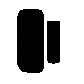
\includegraphics[scale=0.2]{csensor.png} Capteur de contact
      \end{itemize}
    \item Allumer le four.
      \begin{itemize}
      \item 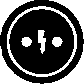
\includegraphics[scale=0.2]{emeter.png} Capteur de consommation électrique.
      \end{itemize}
    \end{itemize}
\end{coloredbox}
  \end{minipage}
  \hfill
  \begin{minipage}{0.50\linewidth}
    \begin{figure}
      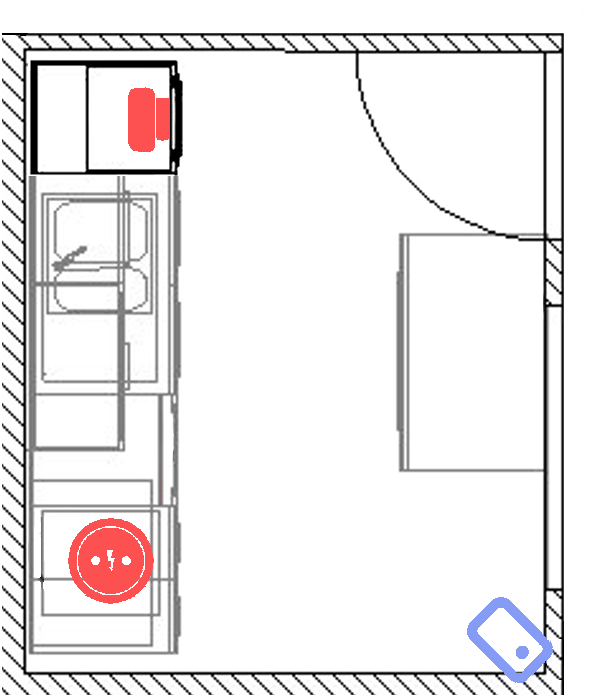
\includegraphics[scale=0.20]{use_case1.png}
    \end{figure}
  \end{minipage}
\end{frame}
% **********************************************
\begin{frame}{Implantation domiciliaire du contexte}
  \addtocounter{framenumber}{-1}
\begin{minipage}{.48\linewidth}
    \begin{coloredbox}[black]{}
      \begin{scriptsize}
        Freezer gets opened and stove gets turned on within 10 minutes during lunch time.
      \end{scriptsize}
    \end{coloredbox}
  \end{minipage}
  \hfill
  \begin{minipage}{.48\linewidth}
    % \begin{scriptsize}
    %   a presence in the Bedroom is true and a presence in the Kitchen is true within 10 minutes
    % \end{scriptsize}
  \end{minipage}
  \vfill
  \begin{minipage}{0.45\linewidth}
    \begin{coloredbox}[teal]{Préparation du déjeuner}
\small
    \begin{itemize}
    \item Ouvrir la porte du congélateur.
      \begin{itemize}
      \item 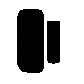
\includegraphics[scale=0.2]{csensor.png} Capteur de contact
      \end{itemize}
    \item Allumer le four.
      \begin{itemize}
      \item 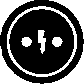
\includegraphics[scale=0.2]{emeter.png} Capteur de consommation électrique.
      \end{itemize}
    \end{itemize}
\end{coloredbox}
  \end{minipage}
  \hfill
  \begin{minipage}{0.50\linewidth}
    \begin{figure}
      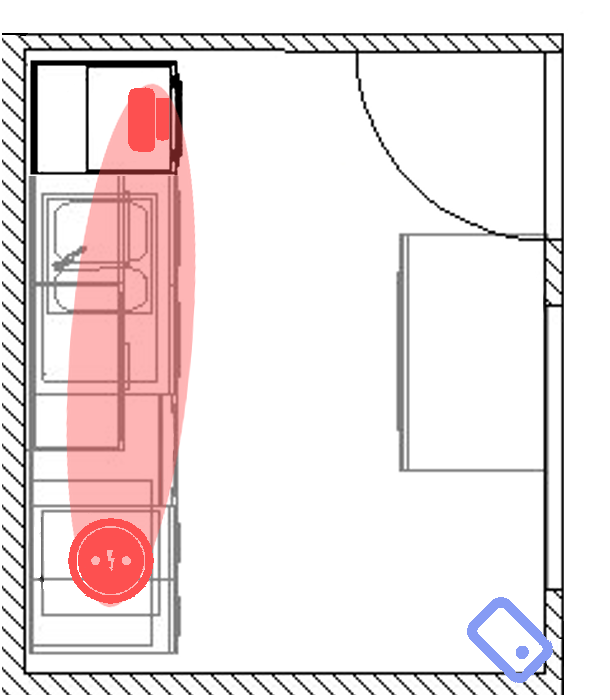
\includegraphics[scale=0.2]{use_case1_5.png}
    \end{figure}
  \end{minipage}
\end{frame}
% **********************************************
\begin{frame}{Implantation domiciliaire du contexte}
  \addtocounter{framenumber}{-1}
  \begin{minipage}{.48\linewidth}
    % \begin{coloredbox}[black]{}
    %   \begin{scriptsize}
    %     Freezer gets opened and stove gets turned on within 10 minutes during lunch time
    %   \end{scriptsize}
    % \end{coloredbox}
  \end{minipage}
  \hfill
  \begin{minipage}{.48\linewidth}
    % \vspace*{2.7mm}
    \begin{coloredbox}[black]{}
      \begin{scriptsize}
        A presence in the Bedroom is true then\\ a presence in the Kitchen is true.% within 10 minutes
      \end{scriptsize}
    \end{coloredbox}
  \end{minipage}
  \vfill

  \begin{minipage}{0.45\linewidth}
    \begin{coloredbox}[teal]{Lever}
      \small
      \begin{itemize}
      \item Présence dans la cuisine.
        \begin{itemize}
        \item 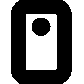
\includegraphics[scale=0.2]{mdetect.png} Capteur de mouvement
        \end{itemize}
        % \item Allumer le four.
        %   \begin{itemize}
        %   \item 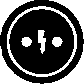
\includegraphics[scale=0.2]{emeter.png} Capteur de consommation électrique.
        %   \end{itemize}
      \end{itemize}
    \end{coloredbox}
  \end{minipage}
  \hfill
  \begin{minipage}{0.50\linewidth}
    \begin{figure}
      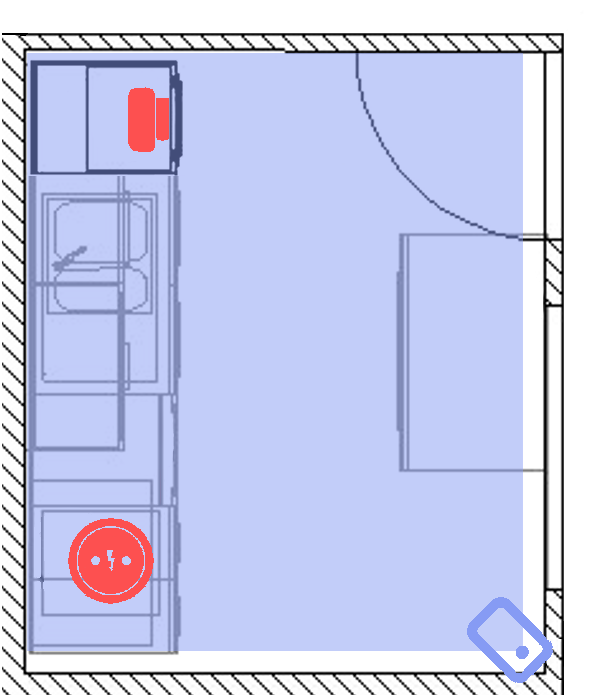
\includegraphics[scale=0.2]{use_case1_2.png}
    \end{figure}
  \end{minipage}
\end{frame}
% **********************************************
\begin{frame}{Implantation domiciliaire du contexte}
  \addtocounter{framenumber}{-1}
\begin{minipage}{.48\linewidth}
    \begin{coloredbox}[black]{}
      \begin{scriptsize}
        Freezer gets opened and stove gets turned on within 10 minutes during lunch time.
      \end{scriptsize}
    \end{coloredbox}
  \end{minipage}
  \hfill
  \begin{minipage}{.48\linewidth}
    \begin{coloredbox}[black]{}
      \begin{scriptsize}
        A presence in the Bedroom is true then\\ a presence in the Kitchen is true.% within 10 minutes
      \end{scriptsize}
    \end{coloredbox}
  \end{minipage}
  \vfill

  \begin{minipage}{0.45\linewidth}
\begin{coloredbox}[teal]{Modèle implicite}
    %Modèle implicite~:
\small
    \begin{itemize}
    \item Détection de mouvement précède toute autre interaction.
    \item Une présence dans une pièce ne peut pas recouvrir une présence dans une autre pièce.
    \end{itemize}
\end{coloredbox}
  \end{minipage}
  \hfill
  \begin{minipage}{0.50\linewidth}
    \begin{figure}
      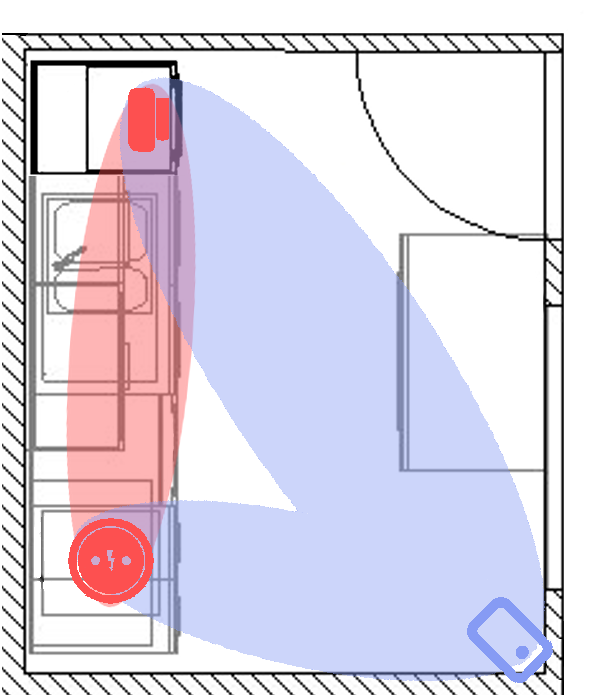
\includegraphics[scale=0.2]{use_case2.png}
    \end{figure}
  \end{minipage}
\end{frame}

% **********************************************


\subsection{Synthèse}
\begin{frame}{Synthèse}
  \begin{minipage}[t]{0.3\linewidth}
    \begin{figure}
      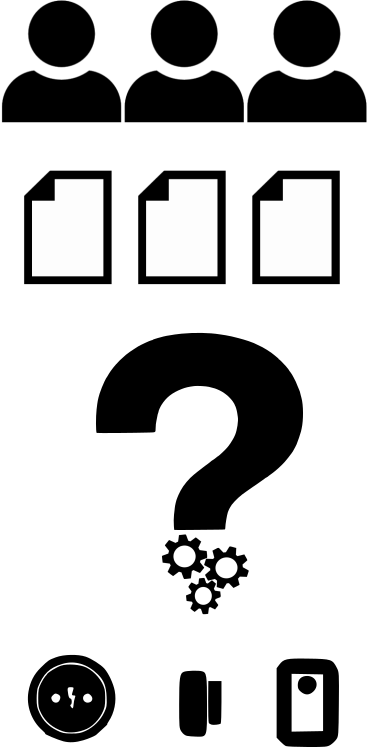
\includegraphics[scale=0.3]{synthese_domain.png}
    \end{figure}
  \end{minipage}
  \begin{minipage}[t]{0.68\linewidth}
    %Besoins:
    \begin{itemize}
      \item Concepts spécifiques au domaine.
      \item Expressivité des services.
    \end{itemize}
    \begin{questionbox}
      Comment couvrir les besoins \\d'expressivité de services sensibles au contexte?
    \end{questionbox}
    \vfill
    \begin{itemize}
      \item Implantation de la sensibilité au contexte.
      \item Modèle implicite.%Fiabilité de la sensibilité au contexte.
    \end{itemize}
    \begin{questionbox}
      Comment rendre explicite le modèle implicite, basé sur les hypothèses?
    \end{questionbox}
  \end{minipage}
\end{frame}
\section{Fiabilité de la sensibilité au contexte}

\begin{frame}{Rendre explicite le modèle implicite}
  \begin{minipage}{0.3\linewidth}
      \begin{figure}
        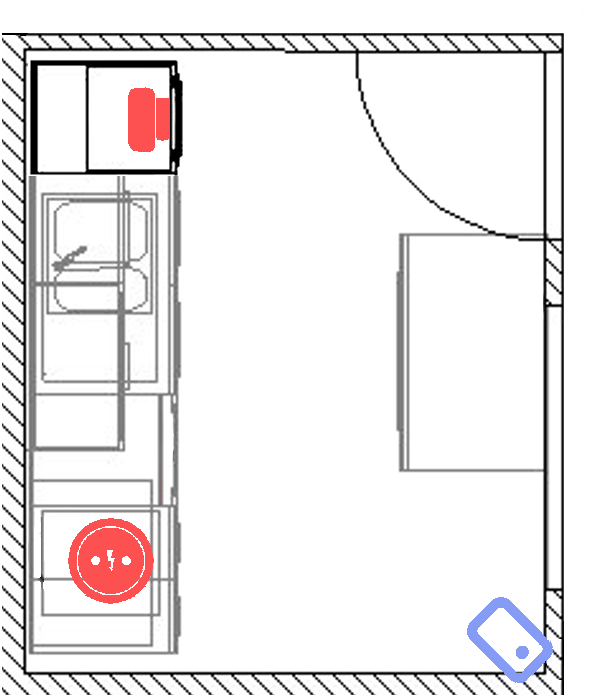
\includegraphics[scale=0.15]{use_case1.png}
      \end{figure}
    \end{minipage}
  \hfill
  \begin{minipage}{0.65\linewidth}
    %\vspace*{-25.9mm}
    \begin{coloredbox}[black]{Dépendance de présence}
      \footnotesize
      Chaque interaction (sauf présence) doit être recouverte par une interaction de présence.
      \small
      \begin{displaymath}
        \begin{array}{c}
        ~\\
        ~
        \end{array}
      \end{displaymath}
    \end{coloredbox}
    \begin{coloredbox}[black]{Non ubiquité}
      \footnotesize
      Une présence ne peut pas être simultanément détectée dans deux endroits différents.
      \small
      \begin{displaymath}
        \begin{array}{c}
         ~\\ 
         ~
        \end{array}
      \end{displaymath}
    \end{coloredbox}
  \end{minipage}
\end{frame}

\begin{frame}{Rendre explicite le modèle implicite}
  \addtocounter{framenumber}{-1}
  \begin{minipage}{0.3\linewidth}
      \begin{figure}
        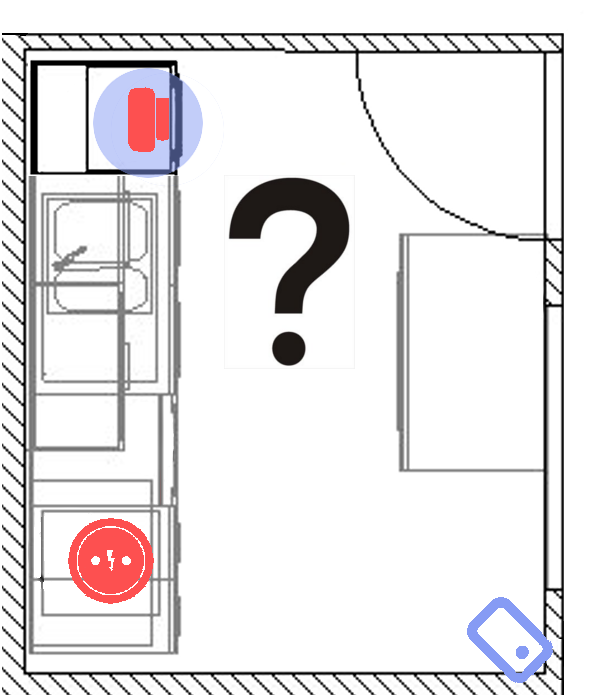
\includegraphics[scale=0.15]{use_case_issue_1.png}
      \end{figure}
    \end{minipage}
  \hfill
  \begin{minipage}{0.65\linewidth}
    %\vspace*{-25.9mm}
    \begin{coloredbox}[black]{Dépendance de présence}
      \footnotesize
      Chaque interaction (sauf présence) doit être recouverte par une interaction de présence.
      \small
      \begin{displaymath}
        \begin{array}{c}
        ~\\
        ~
        \end{array}
      \end{displaymath}
    \end{coloredbox}
    \begin{coloredbox}[black]{Non ubiquité}
      \footnotesize
      Une présence ne peut pas être simultanément détectée dans deux endroits différents.
      \small
      \begin{displaymath}
        \begin{array}{c}
         ~\\ 
         ~
        \end{array}
      \end{displaymath}
    \end{coloredbox}
  \end{minipage}
\end{frame}

\begin{frame}{Rendre explicite le modèle implicite}
  \addtocounter{framenumber}{-1}
  \begin{minipage}{0.3\linewidth}
      \begin{figure}
        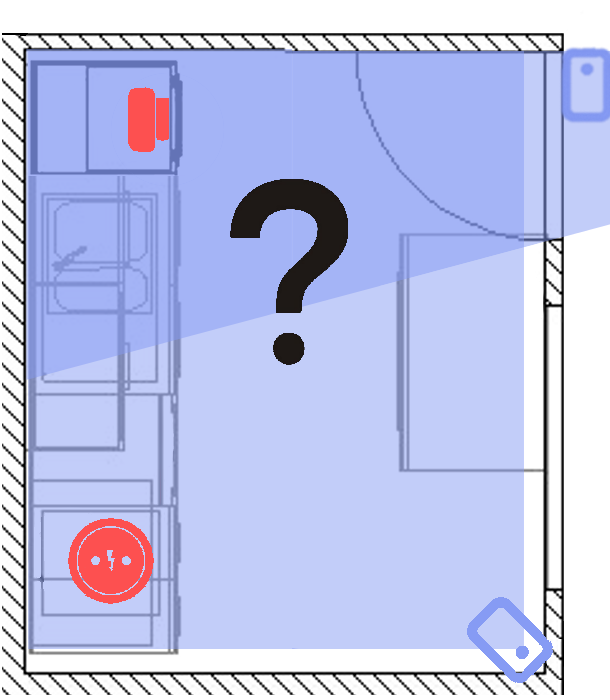
\includegraphics[scale=0.15]{use_case_issue_2.png}
      \end{figure}
    \end{minipage}
  \hfill
  \begin{minipage}{0.65\linewidth}
    %\vspace*{-25.9mm}
    \begin{coloredbox}[black]{Dépendance de présence}
      \footnotesize
      Chaque interaction (sauf présence) doit être recouverte par une interaction de présence.
      \small
      \begin{displaymath}
        \begin{array}{c}
        ~\\
        ~
        \end{array}
      \end{displaymath}
    \end{coloredbox}
    \begin{coloredbox}[black]{Non ubiquité}
      \footnotesize
      Une présence ne peut pas être simultanément détectée dans deux endroits différents.
      \small
      \begin{displaymath}
        \begin{array}{c}
         ~\\ 
         ~
        \end{array}
      \end{displaymath}
    \end{coloredbox}
  \end{minipage}
\end{frame}

\begin{frame}{Rendre explicite le modèle implicite~: Modèle d'infrastructure}
  \addtocounter{framenumber}{-1}
  \begin{minipage}{0.3\linewidth}
      \begin{figure}
        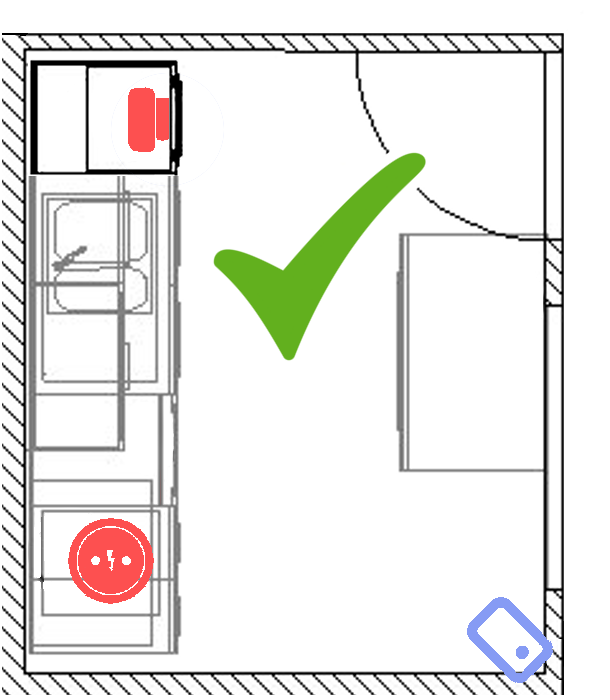
\includegraphics[scale=0.15]{use_case_final.png}
      \end{figure}
    \end{minipage}
  \hfill
  \begin{minipage}{0.65\linewidth}
    \begin{coloredbox}[black]{Dépendance de présence}
      \footnotesize
      Chaque interaction (sauf présence) doit être recouverte par une interaction de présence.
      \small
      \begin{displaymath}
        \begin{array}{c}
          \forall~<k, Kitchen, p>~\in~Log, k \neq Presence~ \Rightarrow \\
          ~~~~\exists~ <Presence, Kitchen, p'>~\in~Log,~p \subseteq p' 
        \end{array}
      \end{displaymath}
    \end{coloredbox}
    \begin{coloredbox}[black]{Non ubiquité}
      \footnotesize
      Une présence ne peut pas être simultanément détectée dans deux endroits différents.
      \small
      \begin{displaymath}
        \begin{array}{c}
          \forall~<Presence, l, p>~\in~Log \Rightarrow \\
          ~~~~\nexists~ <Presence, l', p'>~\in~Log,~l \neq l' \wedge ~p' \cap p \neq \emptyset
        \end{array}
      \end{displaymath}

    \end{coloredbox}
  \end{minipage}
\end{frame}
% **********************************************

% \begin{frame}{Rendre explicite le modèle implicite}
%   % Abstraction de roles de capteurs: {\footnotesize \( e~\in~Event = Kind \times Loc \times Period\)}

%   \begin{minipage}{0.3\linewidth}
%     \onslide<1->{
%       \begin{figure}
%         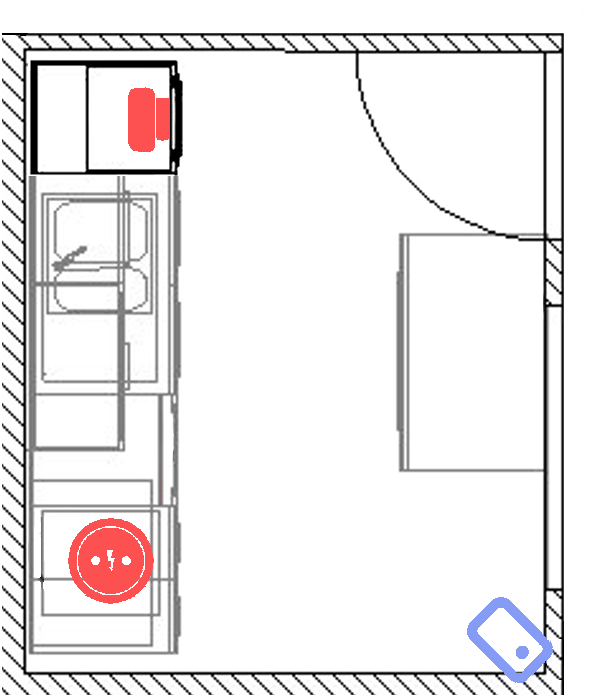
\includegraphics[scale=0.15]{use_case1.png}
%       \end{figure}
%       % \begin{footnotesize}
%       %   \begin{coloredbox}[teal]{Hypothèses}
%       %     \begin{itemize}
%       %     \item Détection de mouvement précède toute autre interaction.
%       %     \item Une présence dans une pièce ne peut pas recouvrir une présence dans une autre pièce.
%       %     \end{itemize}
%       %   \end{footnotesize}
%       }
%     \end{minipage}
%   \hfill
%   \begin{minipage}{0.65\linewidth}
%     \begin{coloredbox}[gray]{Dépendance de présence}
%       \footnotesize
% \onslide<1->{
%       Chaque interaction (sauf présence) doit être recouverte par une interaction de présence.% à la même localisation
%       % Any detected interaction (but presence) must be surrounded by a presence interaction
% }
%       \small
% \onslide<2->{
%       \begin{displaymath}
%         \begin{array}{c}
%           \forall~<k, Kitchen, p>~\in~Log, k \neq Presence~ \Rightarrow \\
%           ~~~~\exists~ <Presence, Kitchen, p'>~\in~Log,~p \subseteq p' 
%         \end{array}
%       \end{displaymath}
% }
%     \end{coloredbox}
%     %\vfill
%     \begin{coloredbox}[gray]{Non ubiquité}
%       \footnotesize
% \onslide<1->{
%       Une présence ne peut pas être simultanément détectée dans deux endroits différents.
% }
%       \small
% \onslide<3->{
%       \begin{displaymath}
%         \begin{array}{c}
%           \forall~<Presence, l, p>~\in~Log \Rightarrow \\
%           ~~~~\nexists~ <Presence, l', p'>~\in~Log,~l \neq l' \wedge ~p' \cap p \neq \emptyset
%         \end{array}
%       \end{displaymath}
% }
%     \end{coloredbox}
%   \end{minipage}
 
% \end{frame}
% **********************************************
% **********************************************
\begin{frame}[fragile]{Validation avec le projet pilote de Domassist}
%\begin{minipage}[t]{0.45\linewidth}
\begin{coloredbox}[black]{Assistance domiciliaire pour personnes âgées}
 % Aims: Aging in place\linebreak
  %\vfill
\footnotesize
  Services définis par des ergothérapeutes, psychologues, experts en vieillissement.\\%\linebreak
  %Activities defined by experts in occupational therapy and psychology and aging\linebreak
  %\vfill
  
  \begin{itemize}
  \item Applications de surveillance des activités du quotidien.
  \item Applications de sécurité du domicile et de l'utilisateur.
  \end{itemize}
  %\vfill
  Étude conduite avec 24 participants vivant seuls pendant 9 mois.
  %Field study: conducted with 24 older participants for a period of 9 months
\end{coloredbox}
\vfill
%\end{minipage}
%\hfill
%\begin{minipage}[t]{0.45\linewidth}
   \begin{table}[!h]
    \begin{scriptsize}
      \begin{tabular}{| c | c |} \hline
        {\bf Name} & {\bf Rule} \\ \hline \hline
        Dépendance de présence & 
$\forall~<i, l, p>~\in~Log, i \neq Presence~ \Rightarrow$\\
        &$~~~\exists~ <Presence, l, p'>~\in~Log,~p \subseteq p'$
%\end{displaymath} 
\\ \hline
        Porte restée ouverte & $\forall~<Opening, l, p>~\in~Log \Rightarrow  \# p < MAX$  \\ \hline
        Non ubiquité & $\forall~<Presence, l, p>~\in~Log \Rightarrow$ \\
     &$~~~~\nexists~ <Presence, l', p'>~\in~Log,~l \neq l' \wedge ~p' \cap p \neq \emptyset$ \\ \hline
         Taux de déclenchement & $\forall~<k, l, p>~\in~Log \Rightarrow$ \\
     &$~~~~~\# (p - Prev(<k, l, p>)) < MAX$ \\ \hline
      \end{tabular}
    \end{scriptsize}
    \vspace{5mm}
    \label{scenario-fig}
    %\caption{Example de scénarios de services d'assistance.}
  \end{table}
%\end{minipage}
\end{frame}
% **********************************************
\begin{frame}{Fiabilité~: Résultats }
  \begin{minipage}[h]{0.45\linewidth}
    \begin{coloredbox}[black]{
        Non-conformités permanentes~:%}
      }
      \onslide<2->{
        %\begin{figure}
          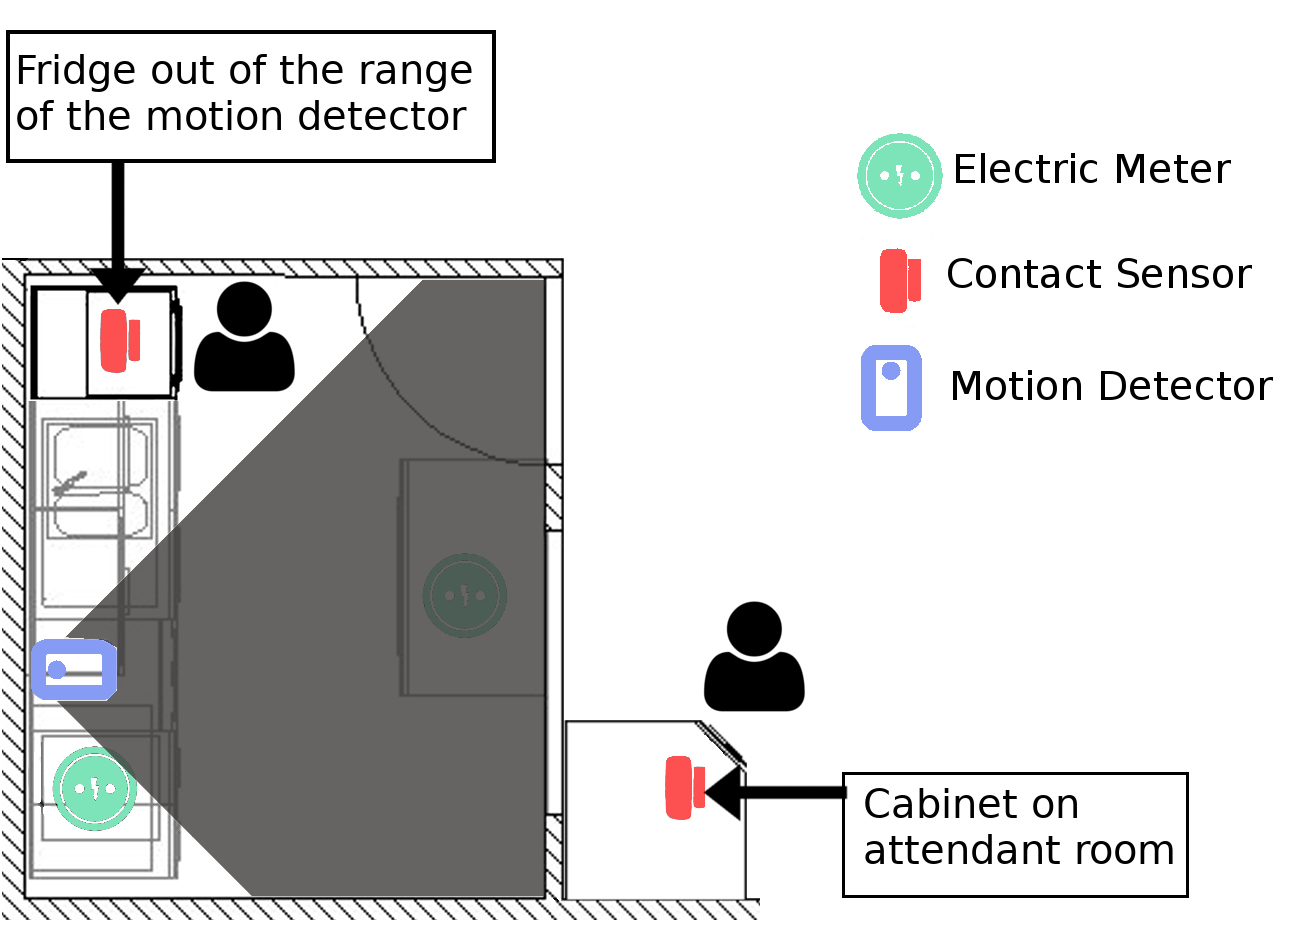
\includegraphics[scale=0.125]{nconf3.png}
          %\label{fig:map}
        %\end{figure}
        \begin{itemize}[label=$\rightarrow$,font=\LARGE \color{black}]
        \item Adapter le modèle.
        \item Repositionner le capteur. 
        \end{itemize}
      }
    \end{coloredbox}
    
  \end{minipage}
  \hfill
  \begin{minipage}[h]{0.45\linewidth}
    \begin{coloredbox}[black]{
        Non-conformités émergentes~: }
      \begin{small}
\onslide<3->{
        \begin{itemize}
        %\item \textbf{Porte restée ouverte~:} \\Chute du capteur de contact.
        \item Chute du capteur de contact.
        %\item \textbf{Dépendance de présence~:}\\Capteur de mouvement défaillant.
        \item Capteur de mouvement défaillant.
%        \item \textbf{Non ubiquité~:}\\Latence des detecteurs de mouvements.

        \end{itemize}
        \vfill
        \begin{itemize}[label=$\rightarrow$,font=\LARGE \color{black}]
        \item Intervention d'un technicien.
        \end{itemize}
}
      \end{small}
    \end{coloredbox}
  \end{minipage}
\end{frame}
% **********************************************
\begin{frame}{Synthèse~: Assurer la fiabilité du contexte\\
Modèle d'infrastructure explicite sous forme de règles~\cite{carteron2016improving}
}
\begin{coloredbox}[checked]{Conformité d'une installation avec un modèle}
%Conformité d'une installation avec un modèle:
  \begin{itemize}%[<+->]
  \item Certifie l'installation.
  \item Guide l'installation.
  \item Application certifiée pour un modèle/installation.
  \end{itemize}
\end{coloredbox}
\vfill
\begin{coloredbox}[checked]{Vérification continue}
%Vérification continue:  
  \begin{itemize}
  \item Détection des pannes.
  \item Aide au diagnostic.
  \end{itemize}
\end{coloredbox}
\vfill

%~\cite{carteron2016improving}
\end{frame}
% **********************************************

% **********************************************
\section{Maloya: langage dédié aux services sensibles au contexte}


\begin{frame}{Une approche dédiée à l'assistance domiciliaire}
\begin{figure}
  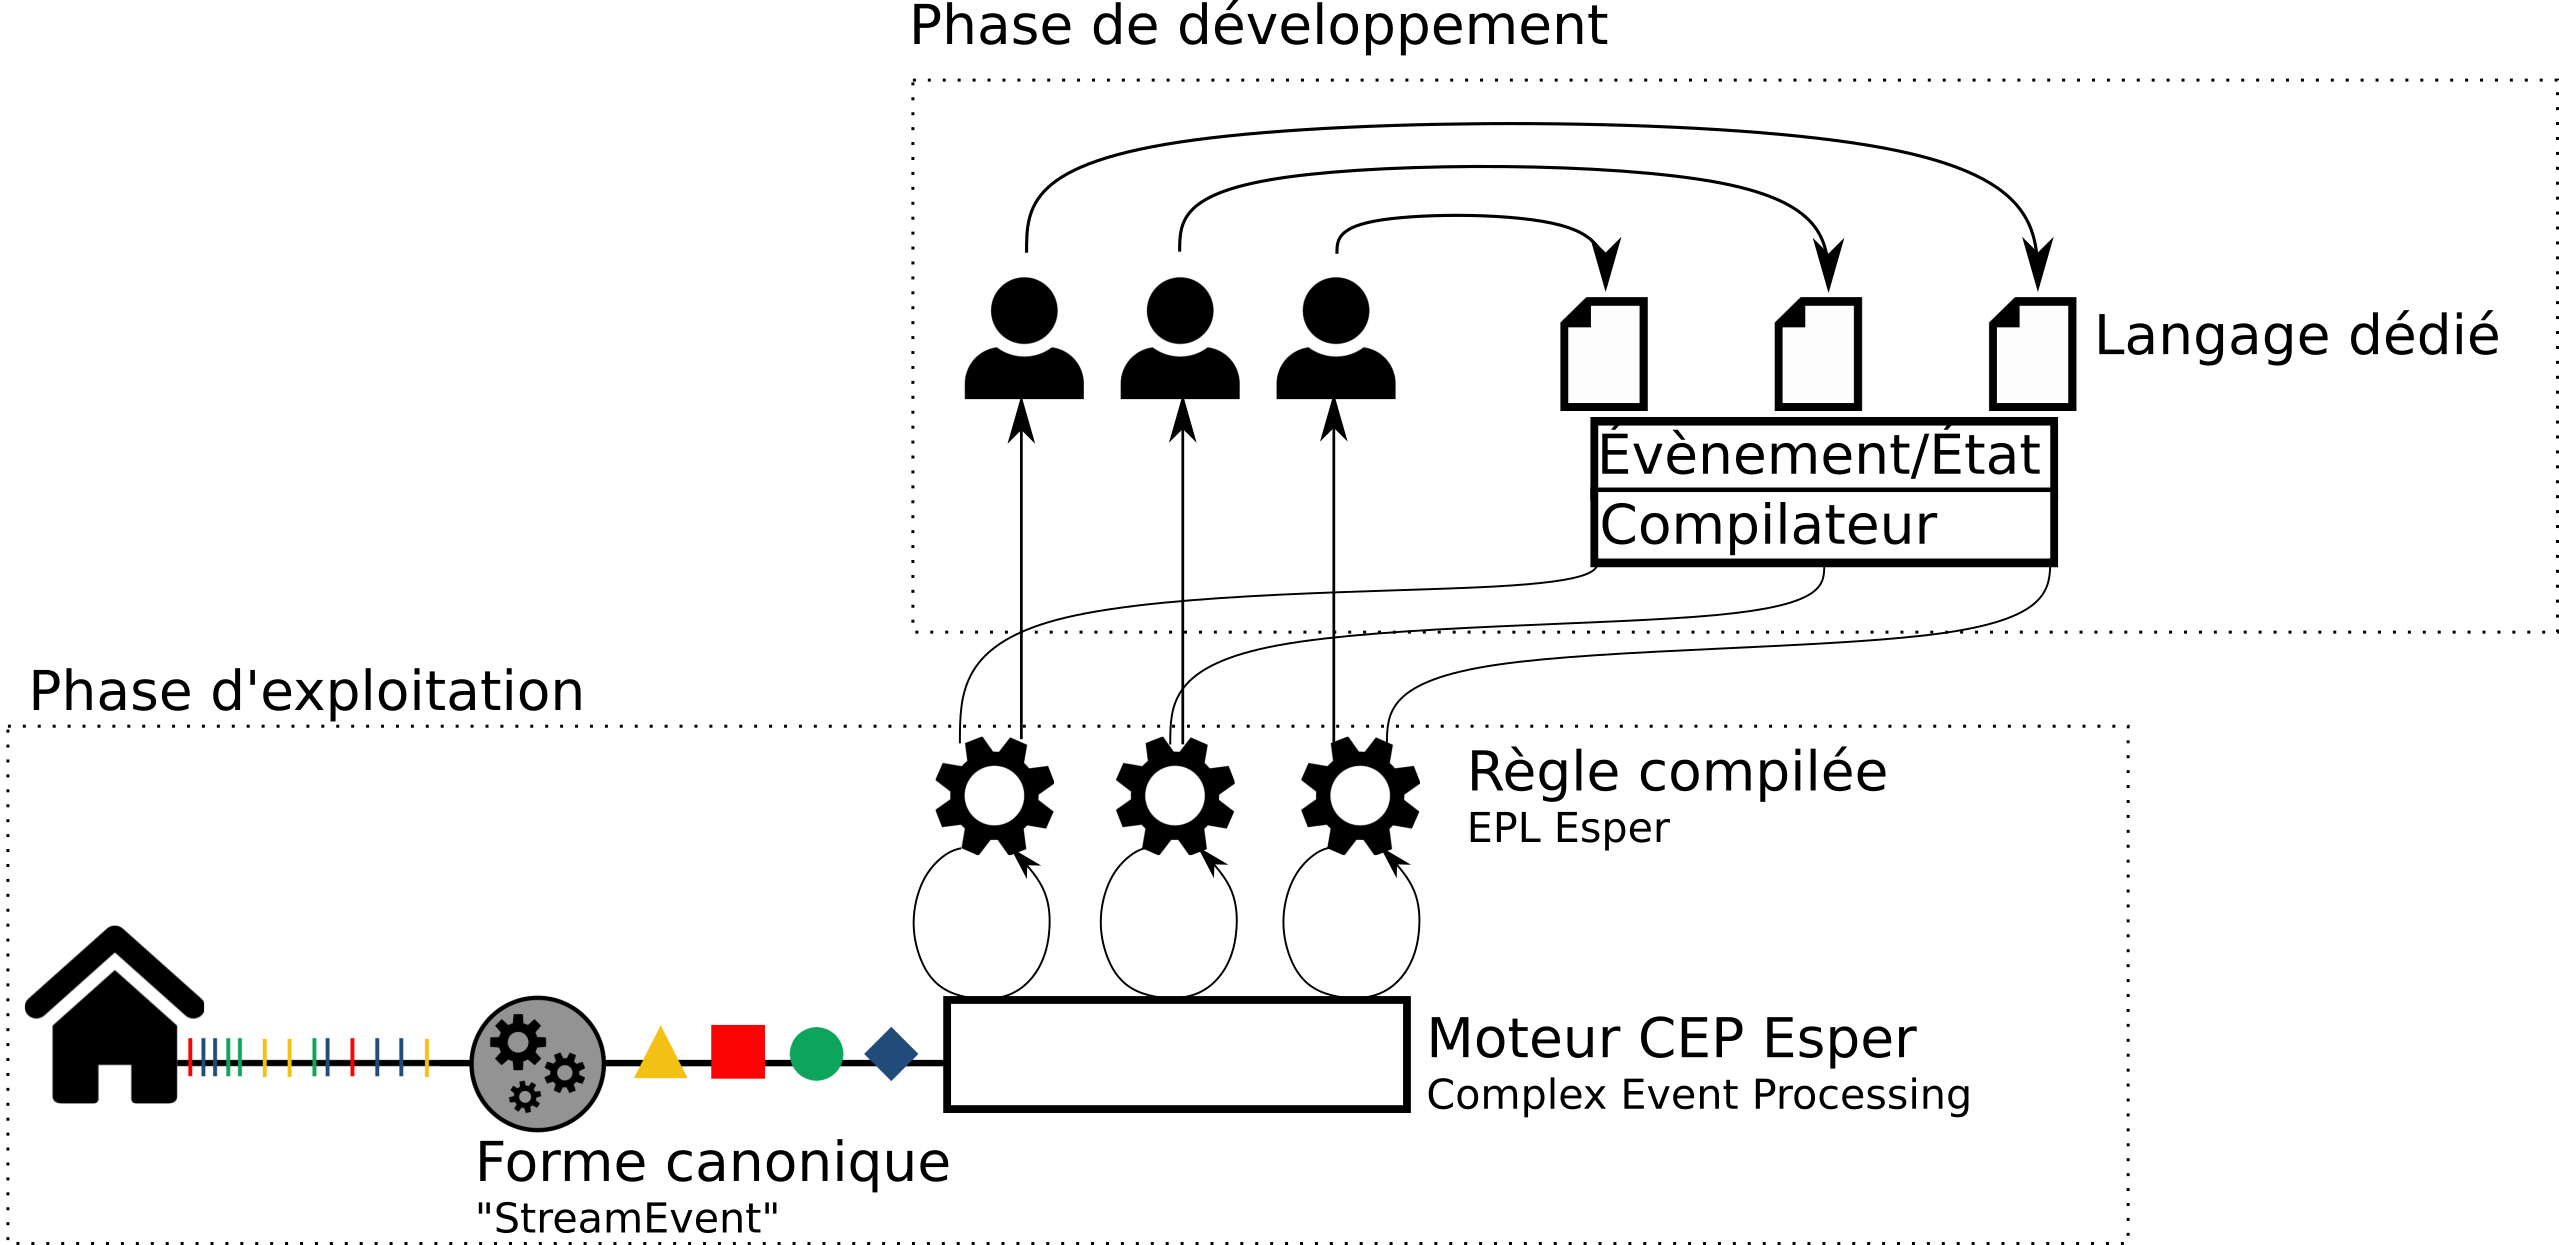
\includegraphics[scale=0.2]{approach_1.png}
\end{figure}
\end{frame}
\begin{frame}{Une approche dédiée à l'assistance domiciliaire}
\addtocounter{framenumber}{-1}
\begin{figure}
  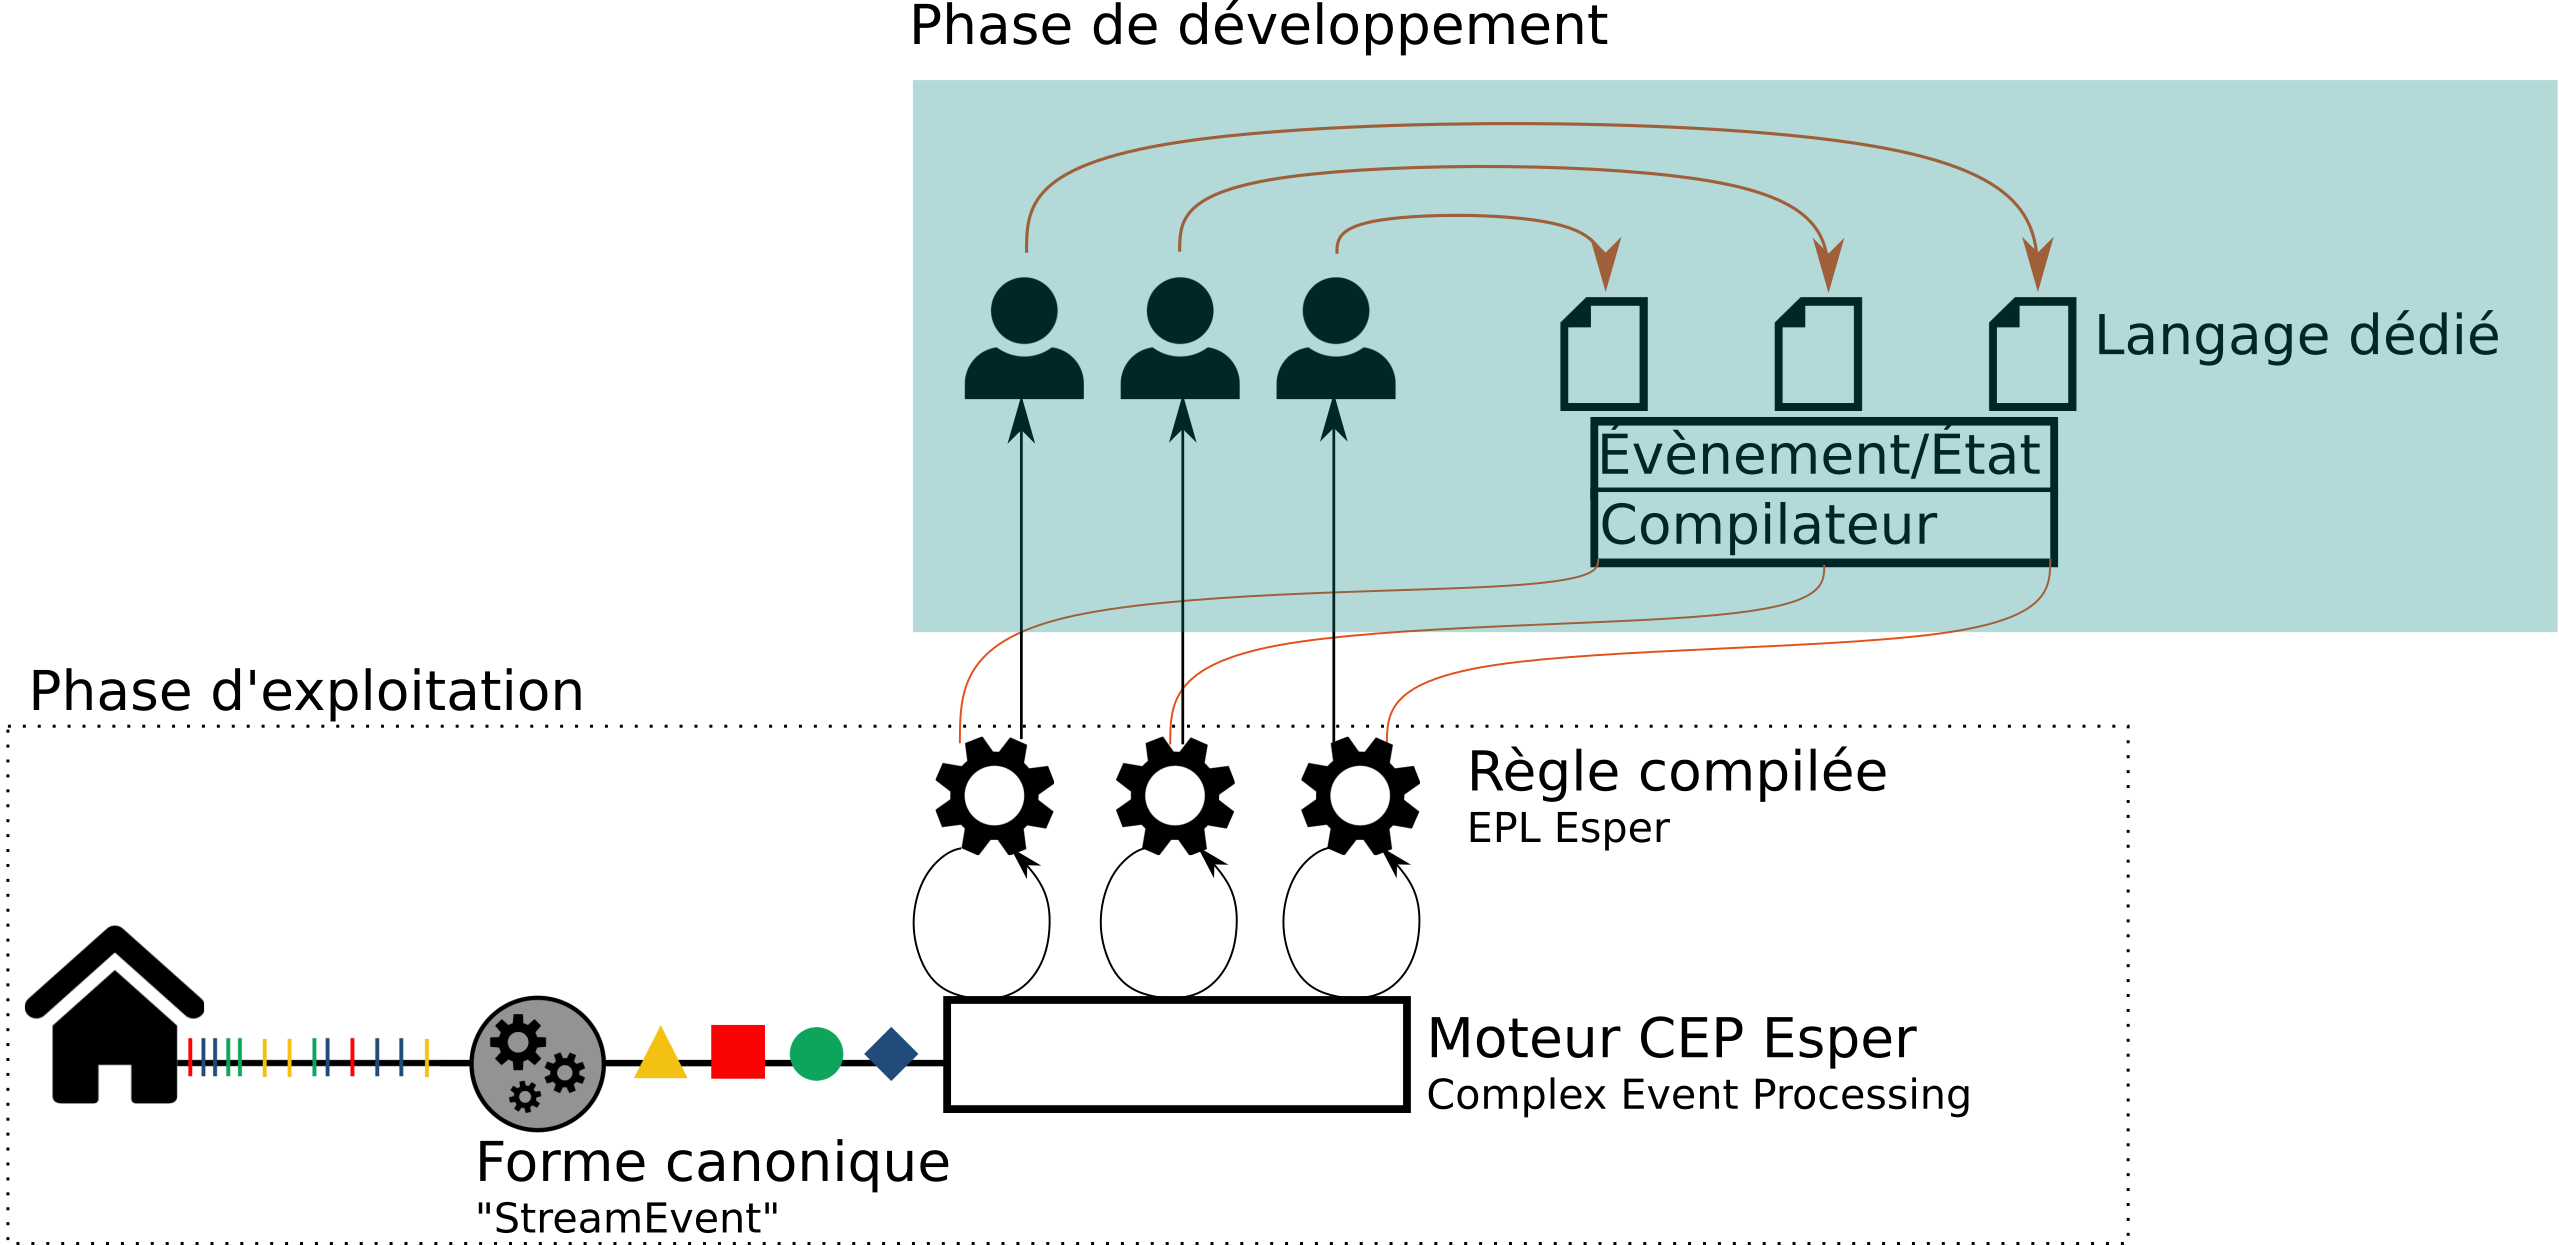
\includegraphics[scale=0.2]{approach_2.png}
\end{figure}
\end{frame}
\begin{frame}{Une approche dédiée à l'assistance domiciliaire}
\addtocounter{framenumber}{-1}
\begin{figure}
  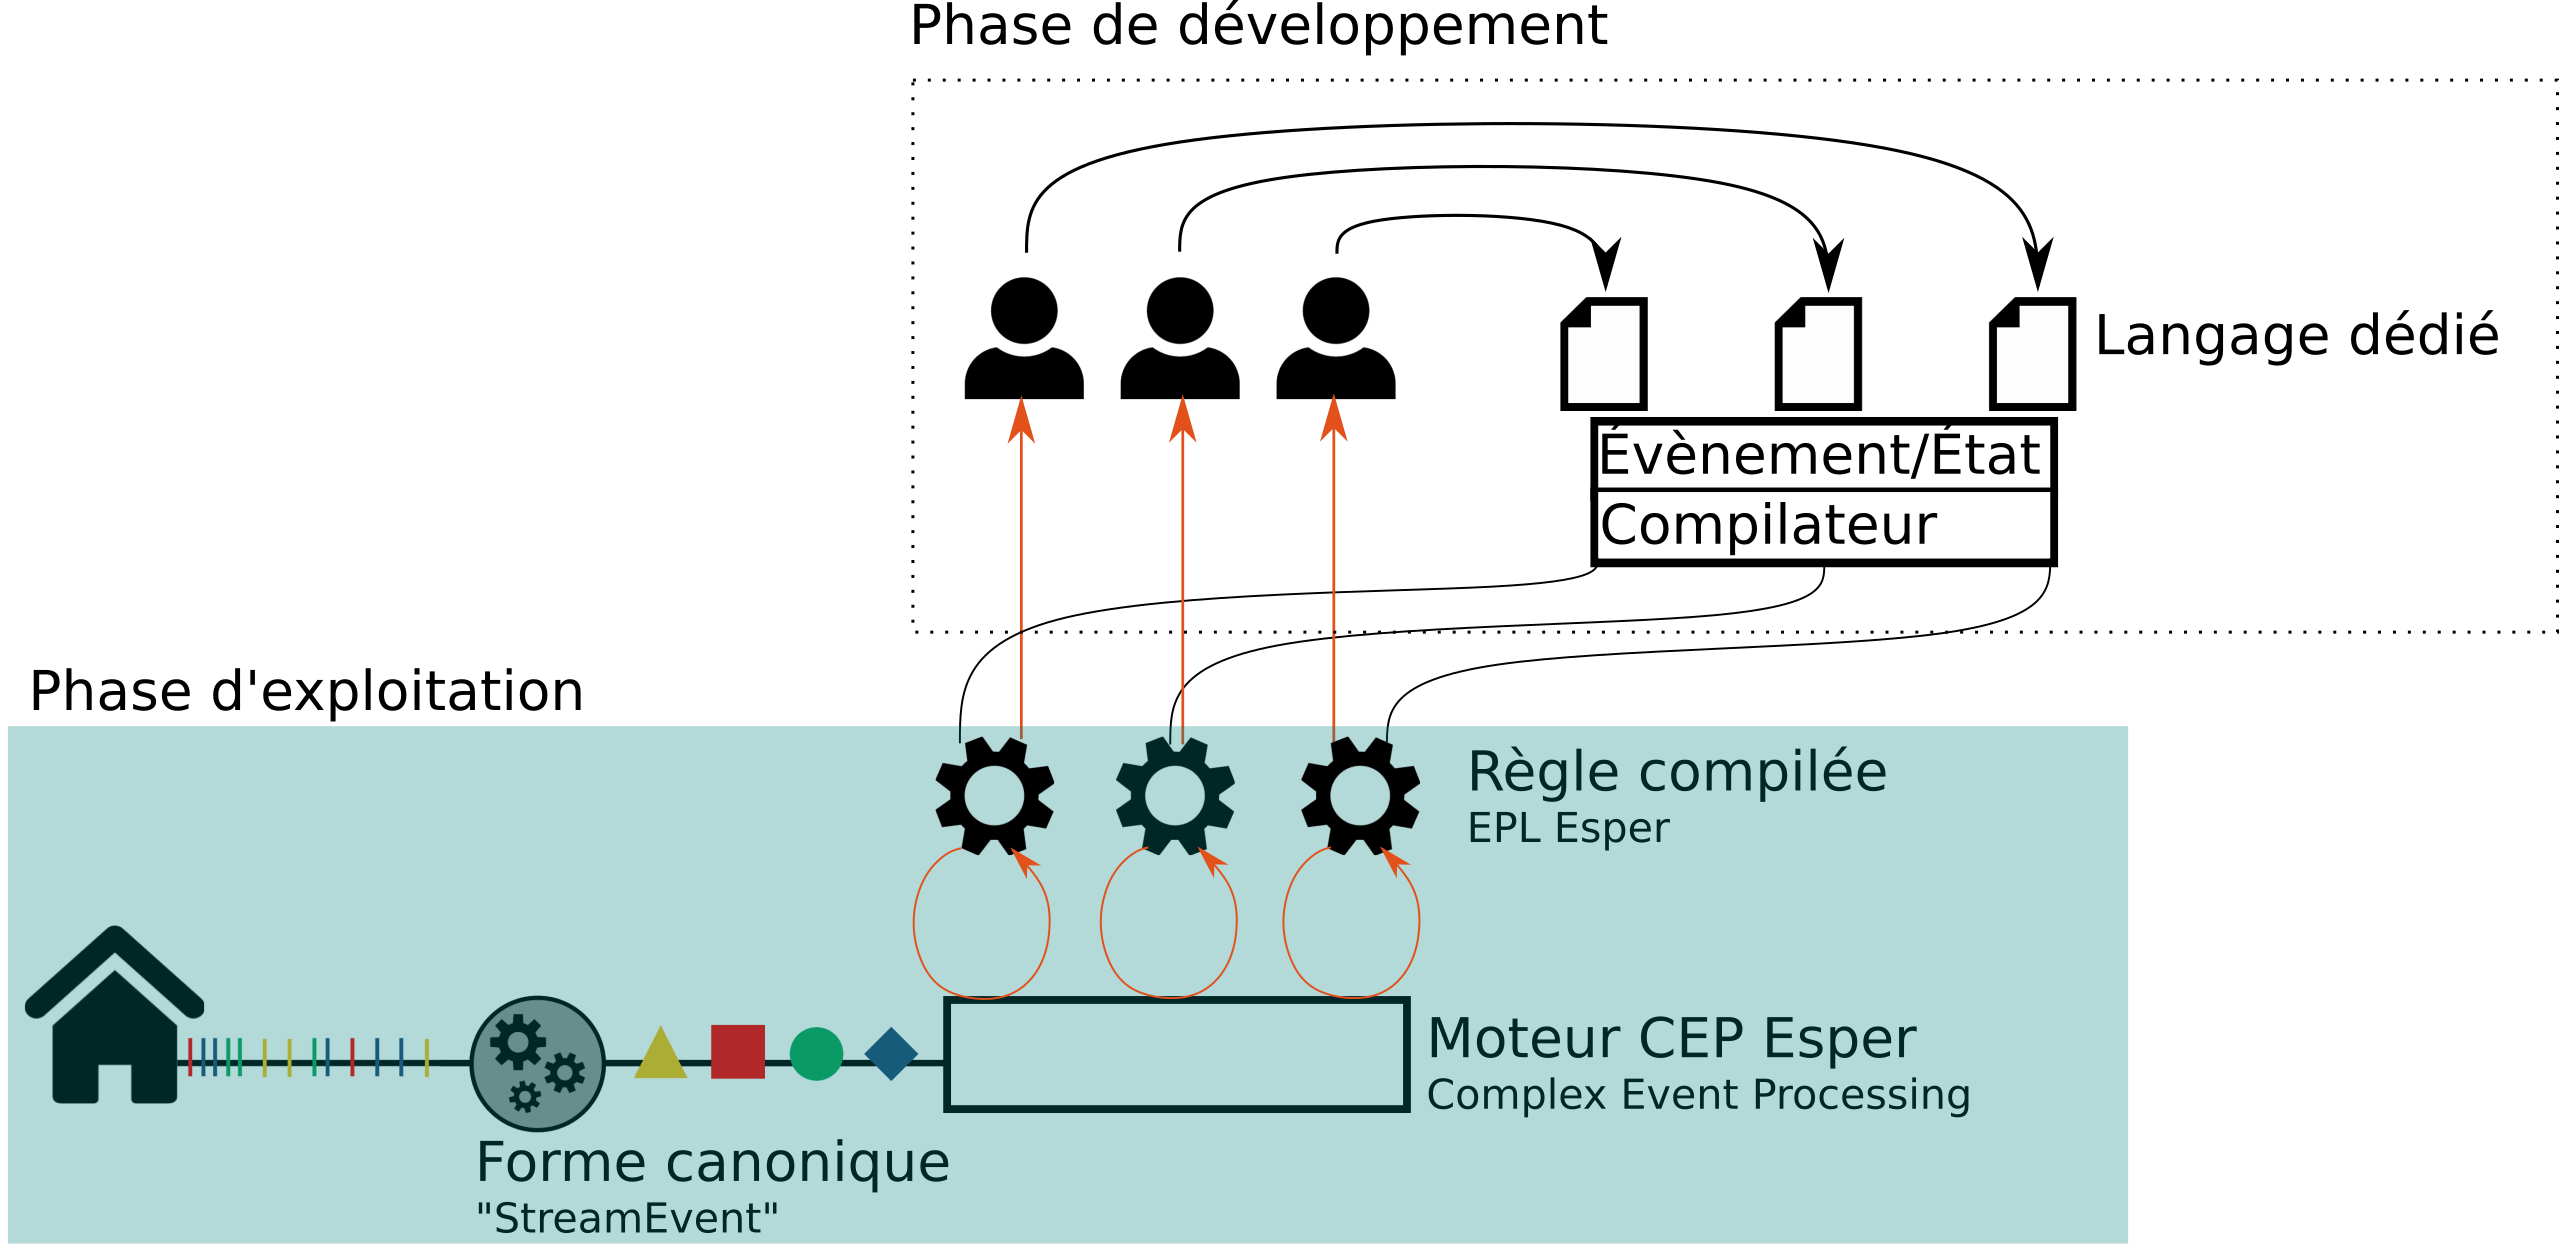
\includegraphics[scale=0.2]{approach_3.png}
\end{figure}
\end{frame}

% \begin{frame}{Scénarios d'assistance domiciliaire}
%   \begin{minipage}[t]{0.45\linewidth}
%     \begin{table}[!h]
%       \begin{footnotesize}
%         \begin{tabular}{| p{2.cm} | p{5.5cm} |} \hline
%           {\bf Nom} & {\bf Description} \\ \hline \hline
%           %Alerte porte d'entrée & Entrance door \colorbox{blue!5}{is open} \colorbox{teal!10}{and}  \colorbox{blue!5}{is unattended} \colorbox{teal!10}{for 5 minutes} \\ \hline
%           Réchauffer un plat surgelé  & Freezer \colorbox{checked!10}{gets used} and stove \colorbox{checked!10}{gets turned on} \colorbox{teal!10}{within 10 minutes} \colorbox{teal!10}{or} Freezer \colorbox{checked!10}{gets used} \colorbox{teal!10}{during} stove \colorbox{blue!5}{is on}, \colorbox{teal!10}{during} \colorbox{blue!5}{lunch time} \\ \hline
%           %Dépendance de présence & The cupboard \colorbox{checked!10}{gets opened} in the kitchen, \colorbox{teal!10}{while} a presence in the kitchen \colorbox{blue!5}{is false} \\ \hline
%           %Échec de communication & A sensor \colorbox{blue!5}{fails to communicate} \colorbox{teal!10}{for 24 hours} %and its status does not \dashuline{get updated} 
%           %\\ \hline
%         \end{tabular}
%       \end{footnotesize}
%     \end{table}
%   \end{minipage}
%   \hfill
%   \begin{minipage}[t]{0.38\linewidth}
%     Commonalités:
%     \begin{itemize}
%     \item Mesures d'environnement (physique et numérique).
%     \item \colorbox{checked!10}{Évènements}.
%     \item \colorbox{blue!5}{États}.
%     \end{itemize}
%     Variabilités:
%     \begin{itemize}
%     \item Niveaux d'abstraction.
%     \item \colorbox{teal!10}{Contraintes d'interactions} (précédence, chevauchement, durée,$~\dots$).
%     \end{itemize}
%   \end{minipage}
% \end{frame}

% \begin{frame}{Scénarios d'assistance domiciliaire}
%   \addtocounter{framenumber}{-1}
%   \begin{minipage}[t]{0.45\linewidth}
%     \begin{table}[!h]
%       \begin{footnotesize}
%         \begin{tabular}{| p{2.cm} | p{5.5cm} |} \hline
%           {\bf Name} & {\bf Description} \\ \hline \hline
%           %Alerte porte d'entrée & Entrance door \colorbox{blue!5}{is open} \colorbox{teal!10}{and}  \colorbox{blue!5}{is unattended} \colorbox{teal!10}{for 5 minutes} \\ \hline
%           \cellcolor{red!10}{Réchauffer un plat surgelé}  & \cellcolor{red!10}{Freezer \colorbox{red!10}{gets used} and stove \colorbox{red!10}{gets turned on} \colorbox{red!10}{within 10 minutes} \colorbox{red!10}{or} Freezer \colorbox{red!10}{gets used} \colorbox{red!10}{during} stove \colorbox{red!10}{is on}, \colorbox{red!10}{during} \colorbox{red!10}{lunch time}} \\ \hline
%           %Dépendance de présence & The cupboard \colorbox{checked!10}{gets opened} in the kitchen, \colorbox{teal!10}{while} a presence in the kitchen \colorbox{blue!5}{is false} \\ \hline
%           %Échec de communication & A sensor \colorbox{blue!5}{fails to communicate} \colorbox{teal!10}{for 24 hours} %and its status does not \dashuline{get updated} 
%           \\ \hline
%         \end{tabular}
%       \end{footnotesize}
%     \end{table}
%   \end{minipage}
%   \hfill
%   \begin{minipage}[t]{0.38\linewidth}
%     Commonalités:
%     \begin{itemize}
%     \item Mesures d'environnement (physique et numérique).
%     \item \colorbox{checked!10}{Évènements}.
%     \item \colorbox{blue!5}{États}.
%     \end{itemize}
%     Variabilités:
%     \begin{itemize}
%     \item Niveaux d'abstraction.
%     \item \colorbox{teal!10}{Contraintes d'interactions} (précédence, chevauchement, durée,$~\dots$).
%     \end{itemize}
%   \end{minipage}
% \end{frame}

\begin{frame}[fragile]{Langage de règles}
  \vspace*{-9.65mm}
  \begin{coloredbox}[gray]{}
    \begin{footnotesize}
      Freezer \colorbox{black!2}{gets opened} \colorbox{black!2}{and} stove gets turned on \colorbox{black!2}{within 10 minutes} or \\Freezer gets opened during stove \colorbox{black!2}{is on}, during lunch time
    \end{footnotesize}
  \end{coloredbox}
  \vfill
  \begin{minipage}{.31\linewidth}
  \end{minipage}
  \hfill
  \begin{minipage}{.31\linewidth} 
  \end{minipage}
  \hfill
  \begin{minipage}{.33\linewidth} 
    \begin{center}
    \end{center}
  \end{minipage}
\end{frame}

\begin{frame}[fragile]{Langage de règles}
  \addtocounter{framenumber}{-1}
  % \vspace*{-3mm}
  \begin{coloredbox}[gray]{}
    \begin{footnotesize}
      Freezer \colorbox{checked!50}{gets opened} \colorbox{black!2}{and} stove gets turned on \colorbox{black!2}{within 10 minutes} or \\Freezer gets opened during stove \colorbox{black!2}{is on}, during lunch time
    \end{footnotesize}
  \end{coloredbox}
  \vfill
  \begin{minipage}{.31\linewidth}
    \begin{coloredbox}[checked]{Évènement~:}
      \begin{lstlisting}[language=MaloyaText]
        //Syntaxe textuelle:
        freezer becomes open
      \end{lstlisting}
      % \begin{lstlisting}[language=Maloya]
      %   //Syntaxe abstraite:
      %   freezer => open
      % \end{lstlisting}
    \end{coloredbox}
  \end{minipage}
  \hfill
  \begin{minipage}{.31\linewidth} 
  \end{minipage}
  \hfill
  \begin{minipage}{.33\linewidth} 
    \begin{center}
    \end{center}
  \end{minipage}
\end{frame}

\begin{frame}[fragile]{Langage de règles}
\addtocounter{framenumber}{-1}
%\vspace*{-3.mm}
  \begin{coloredbox}[gray]{}
    \begin{footnotesize}
      Freezer \colorbox{checked!50}{gets opened} \colorbox{black!2}{and} stove gets turned on \colorbox{black!2}{within 10 minutes} or\\ Freezer gets opened during stove \colorbox{darkgray!50}{is on}, during lunch time
    \end{footnotesize}
  \end{coloredbox}
\vfill
  \begin{minipage}{.31\linewidth}
    \begin{coloredbox}[checked]{Évènement~:}
      \begin{lstlisting}[language=MaloyaText]
        //Syntaxe textuelle:
        freezer becomes open
      \end{lstlisting}
      % \begin{lstlisting}[language=Maloya]
      %   //Syntaxe abstraite:
      %   freezer => open
      % \end{lstlisting}
    \end{coloredbox}
  \end{minipage}
  \hfill
  \begin{minipage}{.31\linewidth}
    \begin{coloredbox}[darkgray]{État~:}
      \begin{lstlisting}[language=MaloyaText]
        //Syntaxe textuelle:
        stove is on
      \end{lstlisting}
      % \begin{lstlisting}[language=Maloya]
      %   //Syntaxe abstraite:
      %   stove = on
      % \end{lstlisting}
    \end{coloredbox}
  \end{minipage}
  \hfill
  \begin{minipage}{.33\linewidth}
    \begin{center}
    \end{center}
  \end{minipage}
\end{frame}


\begin{frame}[fragile]{Langage de règles}
\addtocounter{framenumber}{-1}
  \begin{coloredbox}[gray]{}
    \begin{footnotesize}
      Freezer \colorbox{checked!50}{gets opened} \colorbox{black!2}{and} stove gets turned on \colorbox{black!2}{within 10 minutes} or\\ Freezer gets opened during stove \colorbox{darkgray!50}{is on}, during lunch time
    \end{footnotesize}
  \end{coloredbox}
\vfill
  \begin{minipage}{.31\linewidth}
    \begin{coloredbox}[checked]{Évènement~:}
      \begin{lstlisting}[language=MaloyaText]
        //Syntaxe textuelle:
        freezer becomes open
      \end{lstlisting}
      % \begin{lstlisting}[language=Maloya]
      %   //Syntaxe abstraite:
      %   freezer => open
      % \end{lstlisting}
    \end{coloredbox}
  \end{minipage}
  \hfill
  \begin{minipage}{.31\linewidth}
    \begin{coloredbox}[darkgray]{État~:}
      \begin{lstlisting}[language=MaloyaText]
        //Syntaxe textuelle:
        stove is on
      \end{lstlisting}
      % \begin{lstlisting}[language=Maloya]
      %   //Syntaxe abstraite:
      %   stove = on
      % \end{lstlisting}
    \end{coloredbox}
  \end{minipage}
  \hfill
  \begin{minipage}{.33\linewidth}
  \begin{center}
    \begin{scriptsize}
      % \begin{center}
      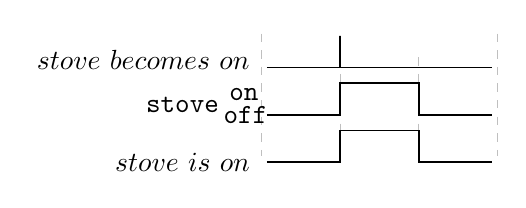
\begin{tikzpicture}[node distance=\dx and \dy,
        >=latex,shorten >=2pt,shorten <=2pt,auto,
        semithick,initial distance=1cm,
        every initial by arrow/.style={*->} ]
        \draw[gray!50,line width=0.1mm,dashed] (-1.5,.5) -- (-1.5,-1.2);
        \draw[gray!50,line width=0.1mm,dashed] (1.5,.5) -- (1.5,-1.2);  
        \draw[gray!50,line width=0.1mm,dashed] (-.5,.2) -- (-.5,-1.);
        \draw[gray!50,line width=0.1mm,dashed] (.5,.2) -- (.5,-1.);  
        \draw[] (-1.5,.) 
        % node[xshift=-3.35 cm,yshift=.125cm] { Évènement~:} 
        %node[xshift=-1.5 cm,yshift=.3cm] { {\tt p {\em becomes} v}} 
        node[xshift=-1.5 cm,yshift=.1 cm] { $stove~becomes~on$} --(-.5,.)--(-.5,.4) -- (-.5,.) -- (1.5,.);
        \draw[] (-1.5,-.6) 
        node[xshift=-.22 cm,yshift=.25cm] { {\tt on}} 
        node[xshift=-.2 cm,yshift=. cm] { {\tt off}} 
        node[xshift=-1. cm,yshift=.125 cm] { {\tt stove}} -- (-.5,-.6) -- (-.5,-.2) -- (.5,-.2) -- (.5,-.6) -- (1.5,-.6);
        \draw[] (-1.5,-1.2) 
        % node[xshift=-3 cm,yshift=.125cm] { État~:} 
        %node[xshift=-1.5 cm,yshift=.3cm] { {\tt p {\em is} v}} 
        node[xshift=-1. cm,yshift=. cm] { $stove~is~on$} -- (-.5,-1.2) -- (-.5,-.8) -- (.5,-.8) -- (.5,-1.2) -- (1.5,-1.2);
      \end{tikzpicture}
    \end{scriptsize}
  \end{center}
\end{minipage}
\end{frame}

\begin{frame}[fragile]{Langage de règles}
  \vspace*{1.4mm}
  \begin{coloredbox}[gray]{}
    \begin{footnotesize}
      Freezer \colorbox{black!2}{gets opened} \colorbox{teal!50}{and} stove gets turned on \colorbox{teal!50}{within 10 minutes} or\\ Freezer gets opened during stove \colorbox{black!2}{is on}, during lunch time
    \end{footnotesize}
  \end{coloredbox}
  \vfill
  \begin{minipage}{.55\linewidth}
    %\vspace*{10.425mm}
    \begin{coloredbox}[teal]{Opérateur Precedes}
      \begin{lstlisting}[language=MaloyaText,basicstyle=\ttfamily\scriptsize]
        //Syntaxe textuelle:
        ( freezer becomes open precedes 
        within 10 minutes stove becomes on )
      \end{lstlisting}
      % \begin{lstlisting}[language=Maloya,basicstyle=\ttfamily\scriptsize]
      %   //Syntaxe abstraite:
      %   Precedes_less(10min)(freezer=>open,stove=>on)
      % \end{lstlisting}
    \end{coloredbox}
  \end{minipage}
  \hfill
  \begin{minipage}{.40\linewidth}

  \end{minipage}
\end{frame}


\begin{frame}[fragile]{Langage de règles}
  \addtocounter{framenumber}{-1}
  \vspace*{3.7mm}
  \begin{coloredbox}[gray]{}
    \begin{footnotesize}
      Freezer \colorbox{black!2}{gets opened} \colorbox{teal!50}{and} stove gets turned on \colorbox{teal!50}{within 10 minutes} or\\ Freezer gets opened during stove \colorbox{black!2}{is on}, during lunch time
    \end{footnotesize}
  \end{coloredbox}
  \vfill
  \begin{minipage}{.55\linewidth}
    %\vspace*{10mm}
    \begin{coloredbox}[teal]{Opérateur Precedes}
      \begin{lstlisting}[language=MaloyaText,basicstyle=\ttfamily\scriptsize]
        //Syntaxe textuelle:
        ( freezer becomes open precedes 
        within 10 minutes stove becomes on )
      \end{lstlisting}
      % \begin{lstlisting}[language=Maloya,basicstyle=\ttfamily\scriptsize]
      %   //Syntaxe abstraite:
      %   Precedes_less(10min)(freezer=>open,stove=>on)
      % \end{lstlisting}
    \end{coloredbox}
  \end{minipage}
  \hfill
  \begin{minipage}{.43\linewidth}
    % \begin{coloredbox}[gray]{}
    \begin{scriptsize}
      % Every time {\tt e$_1$} {\em immediately} precedes {\tt e$_2$}\\
      % \vspace*{3.79mm}
      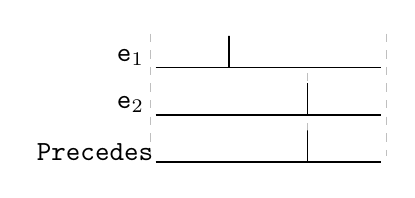
\begin{tikzpicture}[node distance=\dx and \dy,
        >=latex,shorten >=2pt,shorten <=2pt,auto,
        semithick,initial distance=1cm,
        every initial by arrow/.style={*->} ]   
        \draw[gray!50,line width=0.1mm,dashed] (-1.5,.5) -- (-1.5,-1.2);
        \draw[gray!50,line width=0.1mm,dashed] (1.5,.5) -- (1.5,-1.2);  
        %%%%%%%%%%%%%%%%%%%%%%%%%%%%%%%%%%%%%%%%%%%%%%%%%%%%%%%%%%%%%%%%%%%%%%% 
        \draw[gray!50,line width=0.1mm,dashed] (.5,.) -- (.5,-1.2);   
        \draw[] (-1.5,.) 
        node[xshift=-.25 cm,yshift=.125cm] {{\tt e$_1$}}  --(-.5,.)--(-.5,.4) -- (-.5,.) -- (1.5,.);
        \draw[] (-1.5,-.6) 
        node[xshift=-.25 cm,yshift=.125cm] {{\tt e$_2$}} -- (.5,-.6) -- (.5,-.2) -- (.5,-.6) -- (1.5,-.6);
        \draw[] (-1.5,-1.2) 
        % node[xshift=-4.1 cm,yshift=1.cm] {Every time {\tt e$_1$} {\em immediately} precedes {\tt e$_2$}}
        % node[xshift=-3. cm,yshift=.25cm] {{\tt e$_1$ {\bf precedes} e$_2$ $\Leftrightarrow$ $Precedes(e_1,e_2)$}}
        % node[xshift=-6.1 cm,yshift=-.4cm] {Variants:}
        % node[xshift=-1.85 cm,yshift=-.75cm] {{\tt e$_1$ {\bf precedes within} t e$_2$ $\Leftrightarrow$ $Precedes\_less(t)(e_1,e_2)$}}
        % node[xshift=-1.85 cm,yshift=-1.1cm] {{\tt e$_1$ {\bf precedes by} t e$_2$ $\Leftrightarrow$ $Precedes\_greater(t)(e_1,e_2)$}}
        node[xshift=-.7 cm,yshift=.125cm] {{\tt Precedes}} -- (.5,-1.2) -- (.5,-.8) -- (.5,-1.2) -- (1.5,-1.2);
      \end{tikzpicture}

      Variantes~:
      \begin{itemize}
      \item {\tt e$_1$ {\bf precedes within} t e$_2$ }%$\Leftrightarrow$ \\$Precedes\_less(t)(e_1,e_2)$}
      \item {\tt e$_1$ {\bf precedes by} t e$_2$ }%$\Leftrightarrow$ \\$Precedes\_greater(t)(e_1,e_2)$}
      \end{itemize}
    \end{scriptsize}
    % \end{coloredbox}
  \end{minipage}
\end{frame}


% \begin{frame}[fragile]{Langage de règles}
%   \begin{coloredbox}[gray]{Opérateur Occurs}
%     \begin{footnotesize}
%       \begin{tikzpicture}[node distance=\dx and \dy,
%         >=latex,shorten >=2pt,shorten <=2pt,auto,
%         semithick,initial distance=1cm,
%         every initial by arrow/.style={*->} ]  
%         \draw[gray!50,line width=0.1mm,dashed] (-1.5,-7.1) -- (-1.5,-8.7);
%         \draw[gray!50,line width=0.1mm,dashed] (1.5,-7.1) -- (1.5,-8.7);
%         \draw[gray!50,line width=0.1mm,dashed] (-.5,-7.1) -- (-.5,-8.7);
%         \draw[] (-1.5,-7.5) 
%         node[xshift=-.25 cm,yshift=.125cm] {{\tt e}} --(-.5,-7.5)--(-.5,-7.1)--(-.5,-7.5)--(.,-7.5)--(.,-7.1)--(.,-7.5)--(.5,-7.5)--(.5,-7.1)--(.5,-7.5) -- (1.5,-7.5);
%         \draw[] (-1.5,-8.1) 
%         node[xshift=-.25 cm,yshift=.125cm] {{\tt s}} -- (-1.,-8.1) -- (-1.,-7.7) -- (1.,-7.7) -- (1,-8.1) -- (1.5,-8.1);
%         \draw[] (-1.5,-8.7) 
%         node[xshift=-4.5 cm,yshift=1.cm] {La première occurrence d'un évènement {\tt e} durant l'état {\tt s}}
%         node[xshift=-3 cm,yshift=.125cm] {{\tt e {\bf occurs while} s $\Leftrightarrow$ $Occurs(e,s)$}} -- (-.5,-8.7) -- (-.5,-8.3) -- (-.5,-8.7) -- (1.5,-8.7);
%       \end{tikzpicture}
%     \end{footnotesize}
%   \end{coloredbox}
%   \begin{footnotesize}
%     \begin{equation*}
%       \begin{split}
%         \llangle\operatorname{Occurs}(E,[E_{sb},E_{se}])\rrangle(t)=(\exists t_1)(\forall t_2)(&E(t)\wedge \\
%         &(t_1<t) \wedge\\
%         &E_{sb}(t_1)\wedge \\
%         &((t_1<t_2<t)\rightarrow \thicksim (E_{se}(t_2) \vee E(t_2))))
%       \end{split}
%     \end{equation*}
%   \end{footnotesize}
% \end{frame}

\begin{frame}[fragile]{Opérateurs}
  \begin{figure}[!h]
    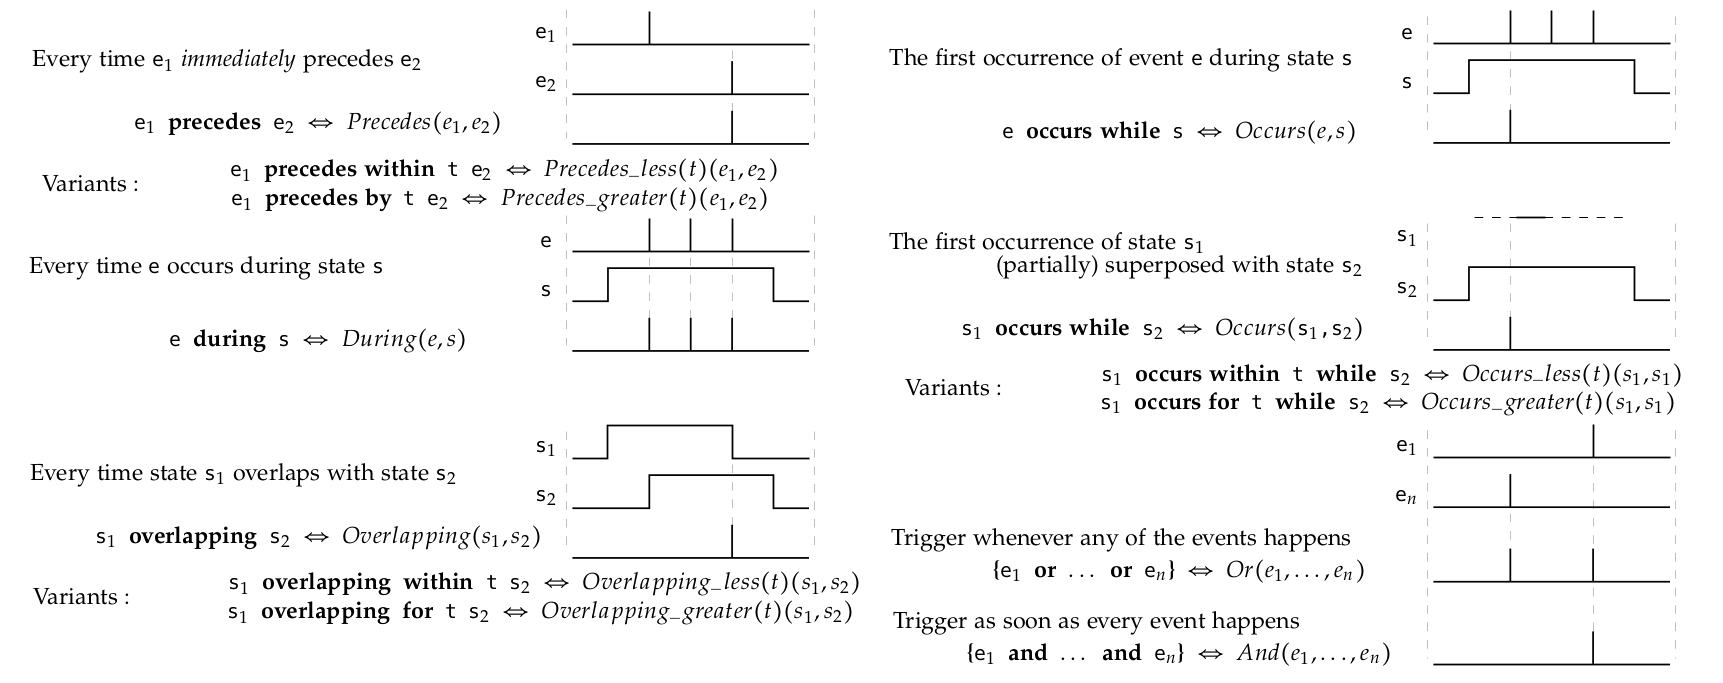
\includegraphics[scale=0.23]{operators.png}
  \end{figure}
\end{frame}
\begin{frame}[fragile]{Opérateurs}
  \addtocounter{framenumber}{-1}
  \begin{figure}[!h]
    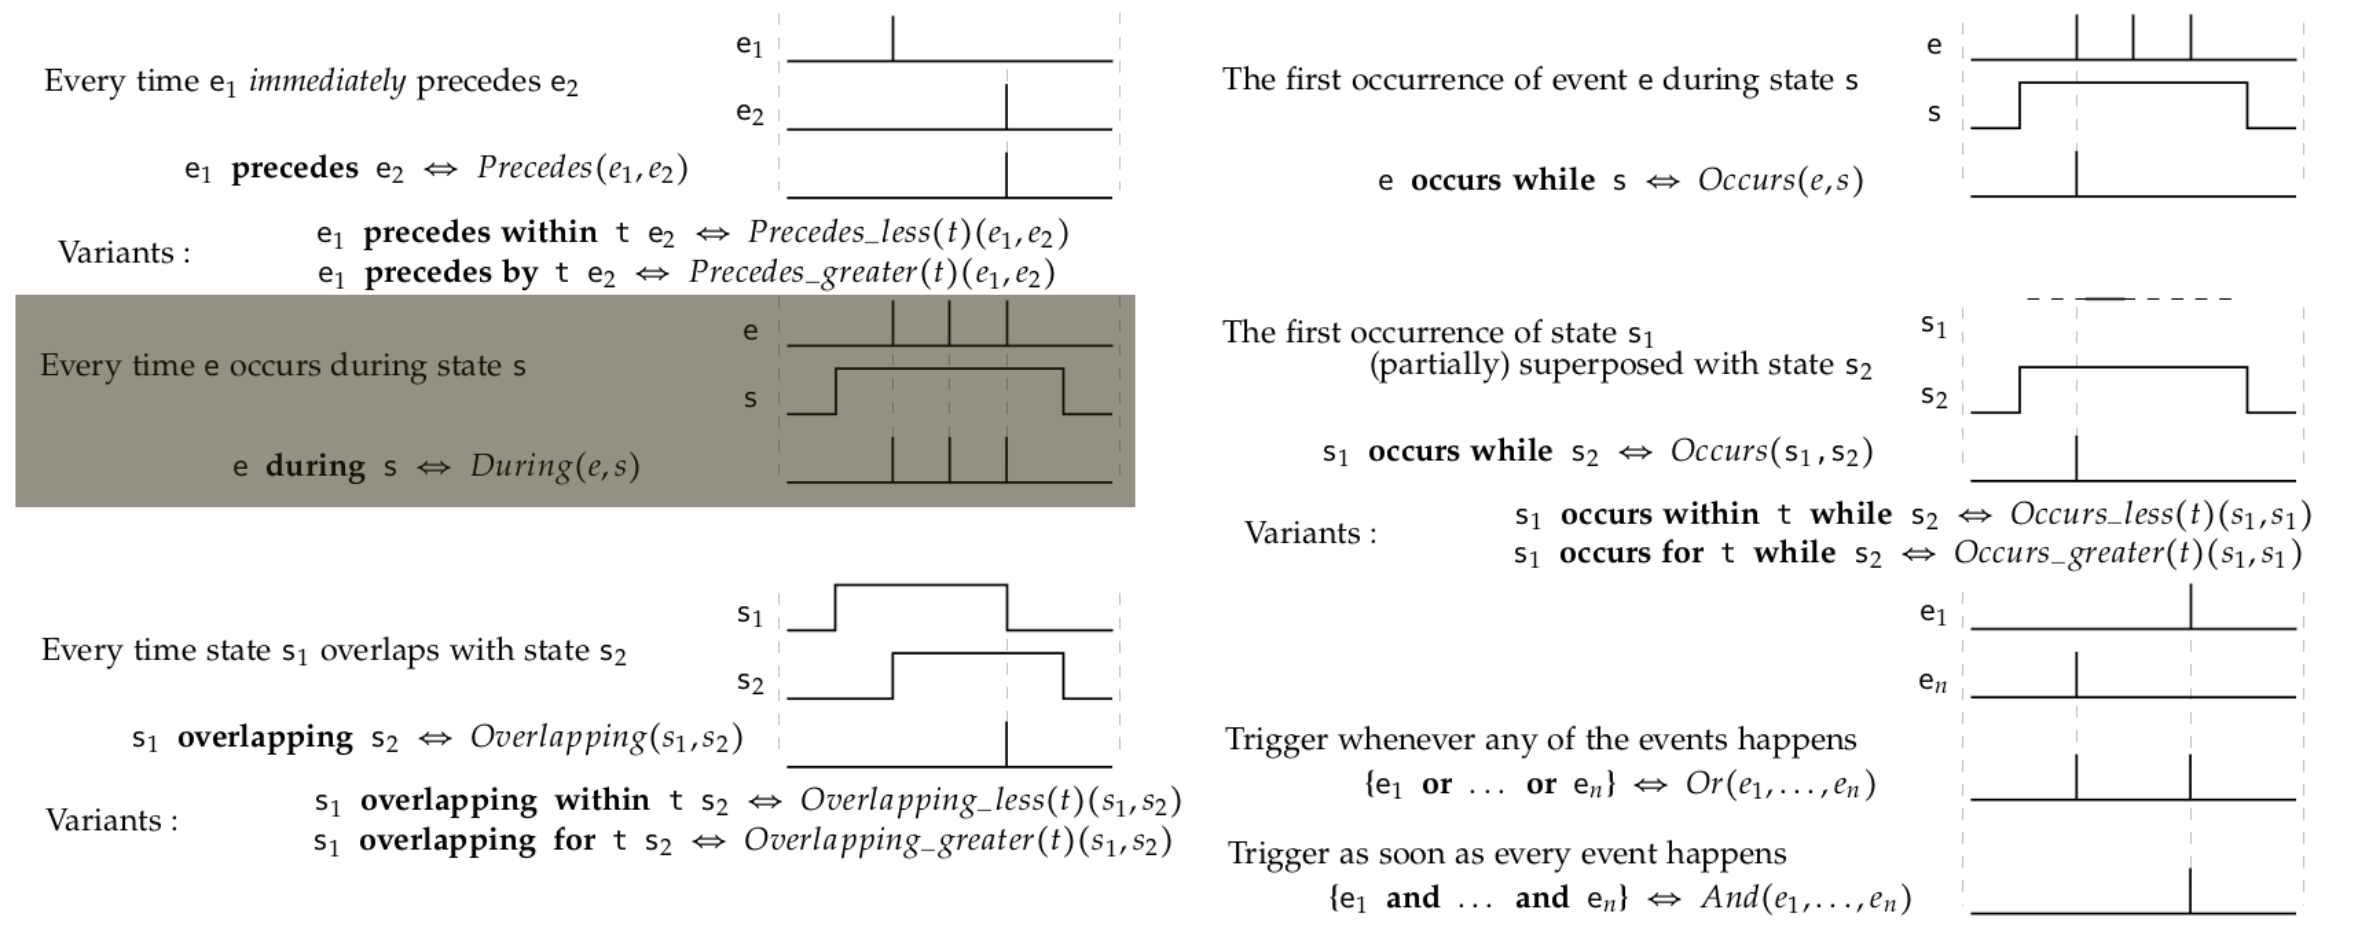
\includegraphics[scale=0.23]{operators_1.png}
  \end{figure}
\end{frame}
\begin{frame}[fragile]{Opérateurs}
  \addtocounter{framenumber}{-1}
  \begin{figure}[!h]
    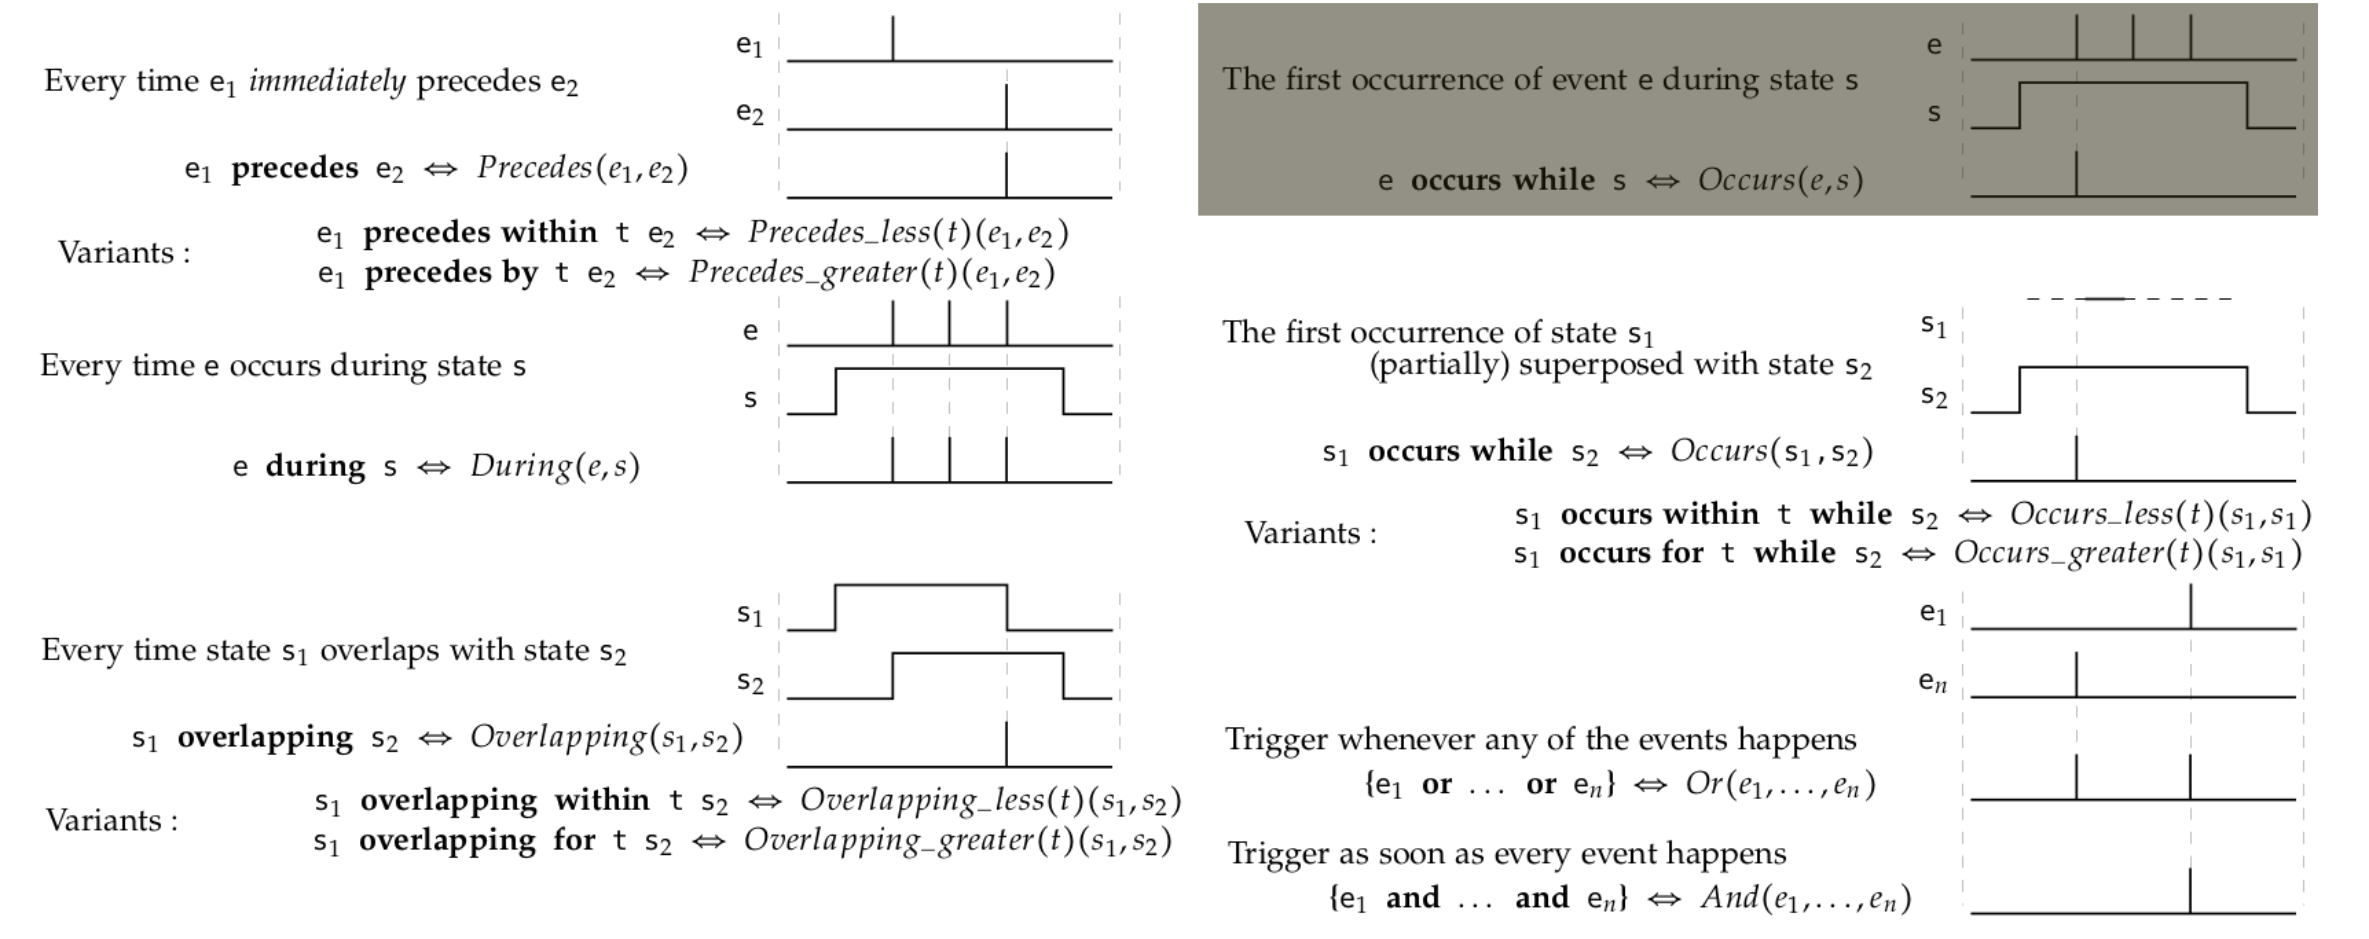
\includegraphics[scale=0.23]{operators_2.png}
  \end{figure}
\end{frame}
\begin{frame}[fragile]{Opérateurs}
  \addtocounter{framenumber}{-1}
  \begin{figure}[!h]
    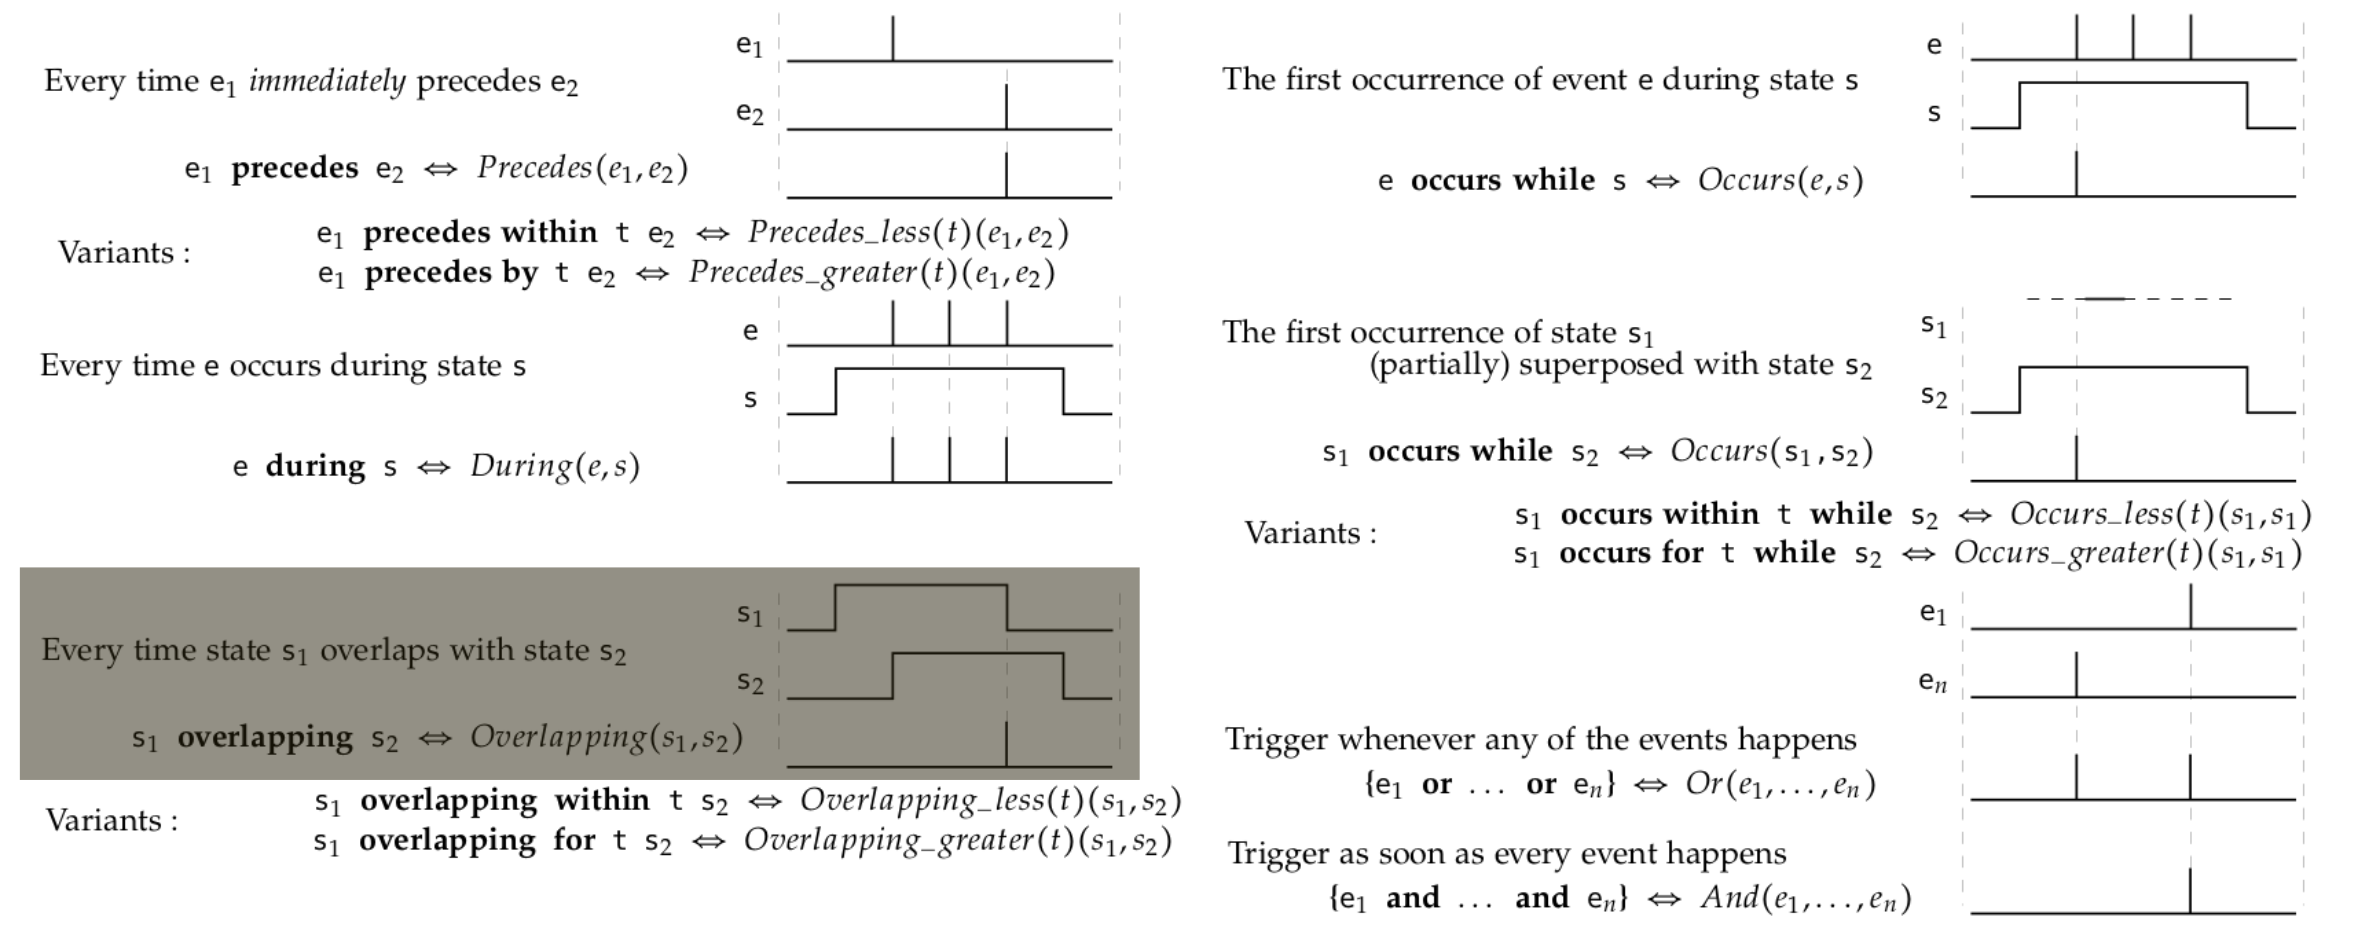
\includegraphics[scale=0.23]{operators_3.png}
  \end{figure}
\end{frame}

% \begin{frame}[fragile]{Définition d'un service}
%   \begin{coloredbox}[gray]{Syntaxe textuelle}
%   \begin{figure}[h]
%     \begin{lstlisting}[language=MaloyaText]
%       { ( freezer becomes open precedes 
%         within 10 minutes stove becomes on )
%         or
%         ( freezer becomes open occurs while stove is on ) 
%       } occurs while lunchTime
%     \end{lstlisting}
%     % \caption{Code Maloya textuel pour le service ``Lunch Reheat''.}
%     \label{listing:maloyaText_reheat} 
%   \end{figure}
% \end{coloredbox}
%  \begin{coloredbox}[gray]{Syntaxe abstraite}
%   \begin{figure}[!h]
%     \begin{lstlisting}[language=Maloya]
%       Occurs(Or(
%         Precedes_less(10min)(freezer => open, stove => on),
%         Occurs(freezer => open, stove = on)),
%       lunchTime)
%     \end{lstlisting}
%     %\caption{Code Maloya interne pour le service ``Lunch Reheat''.}
%     \label{listing:maloya_reheat}
%   \end{figure}
% \end{coloredbox}
% \end{frame}

\begin{frame}[fragile]{Définition d'un service}
  \begin{coloredbox}[black]{Syntaxe textuelle}
  \begin{figure}[h]
    \begin{lstlisting}[language=MaloyaText,basicstyle=\ttfamily\footnotesize,escapechar=!]
      { ( !\colorbox{black!5}{freezer becomes open}! !\colorbox{black!5}{precedes within 10 minutes}! !\colorbox{black!5}{stove becomes on}! )
        !\colorbox{black!5}{or}!
        ( !\colorbox{black!5}{freezer becomes open}! !\colorbox{black!5}{occurs while}! !\colorbox{black!5}{stove is on}! ) 
      } !\colorbox{black!5}{occurs while}! !\colorbox{black!5}{lunchTime}!
    \end{lstlisting}
    % \caption{Code Maloya textuel pour le service ``Lunch Reheat''.}
  \end{figure}
\end{coloredbox}
 \begin{coloredbox}[black]{Syntaxe abstraite}
  \begin{figure}[!h]
    \begin{lstlisting}[language=Maloya,basicstyle=\ttfamily\footnotesize,escapechar=!]
      !\colorbox{black!5}{Occurs}!( !\colorbox{black!5}{Or}!(
        !\colorbox{black!5}{Precedes\_less(10min)}!( !\colorbox{black!5}{freezer => open}!, !\colorbox{black!5}{stove => on}!),
        !\colorbox{black!5}{Occurs}!( !\colorbox{black!5}{freezer => open}!, !\colorbox{black!5}{stove = on}!)),
      !\colorbox{black!5}{lunchTime}!)
    \end{lstlisting}
    %\caption{Code Maloya interne pour le service ``Lunch Reheat''.}
  \end{figure}
\end{coloredbox}
\end{frame}

\begin{frame}[fragile]{Définition d'un service}
\addtocounter{framenumber}{-1}

  \begin{coloredbox}[black]{Syntaxe textuelle}
  \begin{figure}[h]
    \begin{lstlisting}[language=MaloyaText,basicstyle=\ttfamily\footnotesize,escapechar=!]
      { ( !\colorbox{checked!50}{freezer becomes open}! !\colorbox{black!5}{precedes within 10 minutes}! !\colorbox{checked!50}{stove becomes on}! )
        !\colorbox{black!5}{or}!
        ( !\colorbox{checked!50}{freezer becomes open}! !\colorbox{black!5}{occurs while}! !\colorbox{black!5}{stove is on}! ) 
      } !\colorbox{black!5}{occurs while}! !\colorbox{black!5}{lunchTime}!
    \end{lstlisting}
    % \caption{Code Maloya textuel pour le service ``Lunch Reheat''.}
  \end{figure}
\end{coloredbox}
 \begin{coloredbox}[black]{Syntaxe abstraite}
  \begin{figure}[!h]
    \begin{lstlisting}[language=Maloya,basicstyle=\ttfamily\footnotesize,escapechar=!]
      !\colorbox{black!5}{Occurs}!( !\colorbox{black!5}{Or}!(
        !\colorbox{black!5}{Precedes\_less(10min)}!( !\colorbox{checked!50}{freezer => open}!, !\colorbox{checked!50}{stove => on}!),
        !\colorbox{black!5}{Occurs}!( !\colorbox{checked!50}{freezer => open}!, !\colorbox{black!5}{stove = on}!)),
      !\colorbox{black!5}{lunchTime}!)
    \end{lstlisting}
    %\caption{Code Maloya interne pour le service ``Lunch Reheat''.}
  \end{figure}
\end{coloredbox}
\end{frame}

\begin{frame}[fragile]{Définition d'un service}
\addtocounter{framenumber}{-1}

  \begin{coloredbox}[black]{Syntaxe textuelle}
  \begin{figure}[h]
    \begin{lstlisting}[language=MaloyaText,basicstyle=\ttfamily\footnotesize,escapechar=!]
      { ( !\colorbox{checked!50}{freezer becomes open}! !\colorbox{black!5}{precedes within 10 minutes}! !\colorbox{checked!50}{stove becomes on}! )
        !\colorbox{black!5}{or}!
        ( !\colorbox{checked!50}{freezer becomes open}! !\colorbox{black!5}{occurs while}! !\colorbox{black!50}{stove is on}! ) 
      } !\colorbox{black!5}{occurs while}! !\colorbox{black!50}{lunchTime}!
    \end{lstlisting}
    % \caption{Code Maloya textuel pour le service ``Lunch Reheat''.}
  \end{figure}
\end{coloredbox}
 \begin{coloredbox}[black]{Syntaxe abstraite}
  \begin{figure}[!h]
    \begin{lstlisting}[language=Maloya,basicstyle=\ttfamily\footnotesize,escapechar=!]
      !\colorbox{black!5}{Occurs}!( !\colorbox{black!5}{Or}!(
        !\colorbox{black!5}{Precedes\_less(10min)}!( !\colorbox{checked!50}{freezer => open}!, !\colorbox{checked!50}{stove => on}!),
        !\colorbox{black!5}{Occurs}!( !\colorbox{checked!50}{freezer => open}!, !\colorbox{black!50}{stove = on}!)),
      !\colorbox{black!50}{lunchTime}!)
    \end{lstlisting}
    %\caption{Code Maloya interne pour le service ``Lunch Reheat''.}
  \end{figure}
\end{coloredbox}
\end{frame}

\begin{frame}[fragile]{Définition d'un service}
\addtocounter{framenumber}{-1}

  \begin{coloredbox}[black]{Syntaxe textuelle}
  \begin{figure}[h]
    \begin{lstlisting}[language=MaloyaText,basicstyle=\ttfamily\footnotesize,escapechar=!]
      { ( !\colorbox{checked!50}{freezer becomes open}! !\colorbox{teal!50}{precedes within 10 minutes}! !\colorbox{checked!50}{stove becomes on}! )
        !\colorbox{teal!50}{or}!
        ( !\colorbox{checked!50}{freezer becomes open}! !\colorbox{teal!50}{occurs while}! !\colorbox{black!50}{stove is on}! ) 
      } !\colorbox{teal!50}{occurs while}! !\colorbox{black!50}{lunchTime}!
    \end{lstlisting}
    % \caption{Code Maloya textuel pour le service ``Lunch Reheat''.}
  \end{figure}
\end{coloredbox}
 \begin{coloredbox}[black]{Syntaxe abstraite}
  \begin{figure}[!h]
    \begin{lstlisting}[language=Maloya,basicstyle=\ttfamily\footnotesize,escapechar=!]
      !\colorbox{teal!50}{Occurs}!( !\colorbox{teal!50}{Or}!(
        !\colorbox{teal!50}{Precedes\_less(10min)}!( !\colorbox{checked!50}{freezer => open}!, !\colorbox{checked!50}{stove => on}!),
        !\colorbox{teal!50}{Occurs}!( !\colorbox{checked!50}{freezer => open}!, !\colorbox{black!50}{stove = on}!)),
      !\colorbox{black!50}{lunchTime}!)
    \end{lstlisting}
    %\caption{Code Maloya interne pour le service ``Lunch Reheat''.}
  \end{figure}
\end{coloredbox}
\end{frame}


\begin{frame}[fragile]{Étapes de compilation}
  \begin{minipage}{.45\linewidth}
    %\begin{minipage}[t]{.6\linewidth}
      \vspace*{-34.28mm}
      \begin{coloredbox}[black]{\tiny Syntaxe abstraite~:}
      \begin{lstlisting}[language=Maloya,basicstyle=\ttfamily\tiny,escapechar=!]
Occurs(!\colorbox{black!5}{Precedes}!_!\colorbox{black!5}{{\bf less(}10min{\bf )}}!(freezer=>open,
                                !\colorbox{black!5}{stove=>on}!),
       !\colorbox{black!5}{lunchTime}!)
     \end{lstlisting}
\end{coloredbox}
   %\end{minipage}
   \vfill
   %\begin{minipage}[t]{.6\linewidth}
   %\end{minipage}
 \end{minipage}
 \hfill
 \begin{minipage}{.52\linewidth}
   \begin{tiny}
   \end{tiny}
 \end{minipage}
\end{frame}
%*******************************************************************

\begin{frame}[fragile]{Étapes de compilation~: Vers Pseudo-code EPL}
  \begin{minipage}{.45\linewidth}
\vspace*{3.4mm}
    %\begin{minipage}[t]{.6\linewidth}
      \begin{coloredbox}[black]{\tiny Syntaxe abstraite~:}
      \begin{lstlisting}[language=Maloya,basicstyle=\ttfamily\tiny,escapechar=!]
Occurs(!\colorbox{black!5}{Precedes}!_!\colorbox{black!5}{{\bf less(}10min{\bf )}}!(freezer=>open,
                                !\colorbox{black!5}{stove=>on}!),
       !\colorbox{black!5}{lunchTime}!)
     \end{lstlisting}
\end{coloredbox}
   %\end{minipage}
   \vfill
   %\begin{minipage}[t]{.6\linewidth}
            \begin{coloredbox}[black]{\tiny Pseudo-code EPL~:}
     \begin{lstlisting}[language=EPLPseudoCode,basicstyle=\ttfamily\tiny,escapechar=!]
//Window1
( every freezer => open -> !\colorbox{black!5}{stove => on}! 
  and not (freezer=>open)!\colorbox{black!5}{{\bf where timer:within(}10min{\bf )}}!) 

every !\colorbox{black!5}{lunchTime=>begin}! ->
  !\colorbox{black!5}{Window1}!(timestamp > (lunchTime=>begin).timestamp)
  !\colorbox{black!5}{{\bf {\it and not}} lunchTime=>end }!
     \end{lstlisting}
\end{coloredbox}
   %\end{minipage}
 \end{minipage}
 \hfill
 \begin{minipage}{.52\linewidth}
 \end{minipage}
\end{frame}
%*******************************************************************

\begin{frame}[fragile]{Étapes de compilation~: Vers Pseudo-code EPL}
\addtocounter{framenumber}{-1}
\vspace*{3.4mm}
  \begin{minipage}{.45\linewidth}
      \begin{coloredbox}[black]{\tiny Syntaxe abstraite~:}
      \begin{lstlisting}[language=Maloya,basicstyle=\ttfamily\tiny,escapechar=!]
Occurs(!\colorbox{black!5}{Precedes}!_!\colorbox{black!5}{{\bf less(}10min{\bf )}}!(freezer=>open,
                                !\colorbox{black!5}{stove=>on}!),
       !\colorbox{black!50}{lunchTime}!)
      \end{lstlisting}
\end{coloredbox}
    %\end{minipage}
    \vfill
    %\begin{minipage}[t]{.6\linewidth}
            \begin{coloredbox}[black]{\tiny Pseudo-code EPL~:}
      \begin{lstlisting}[language=EPLPseudoCode,basicstyle=\ttfamily\tiny,escapechar=!]
//Window1
( every freezer => open -> !\colorbox{black!5}{stove => on}! 
  and not (freezer=>open)!\colorbox{black!5}{{\bf where timer:within(}10min{\bf )}}!) 

every !\colorbox{black!50}{lunchTime=>begin}! ->
  !\colorbox{black!5}{Window1}!(timestamp > (lunchTime=>begin).timestamp)
  !\colorbox{black!50}{{\bf {\it and not}} lunchTime=>end }!
      \end{lstlisting}
\end{coloredbox}
    %\end{minipage}
  \end{minipage}
  \hfill
  \begin{minipage}{.52\linewidth}
    \vspace*{-69.1mm}
    \begin{tiny}
      \colorbox{black!50}{Gestion des états}
    \end{tiny}
  \end{minipage}
\end{frame}
%*******************************************************************

\begin{frame}[fragile]{Étapes de compilation~: Vers Pseudo-code EPL}
\addtocounter{framenumber}{-1}
\vspace*{3.4mm}
  \begin{minipage}{.45\linewidth}
      \begin{coloredbox}[black]{\tiny Syntaxe abstraite~:}
      \begin{lstlisting}[language=Maloya,basicstyle=\ttfamily\tiny,escapechar=!]
Occurs(!\colorbox{teal!50}{Precedes}!_!\colorbox{black!5}{{\bf less(}10min{\bf )}}!(freezer=>open,
                                !\colorbox{black!5}{stove=>on}!),
       !\colorbox{black!50}{lunchTime}!)
      \end{lstlisting}
\end{coloredbox}
    \vfill
            \begin{coloredbox}[black]{\tiny Pseudo-code EPL~:}
      \begin{lstlisting}[language=EPLPseudoCode,basicstyle=\ttfamily\tiny,escapechar=!]
//Window1
( every freezer => open -> !\colorbox{black!5}{stove => on}! 
  and not (freezer=>open)!\colorbox{black!5}{{\bf where timer:within(}10min{\bf )}}!) 

every !\colorbox{black!50}{lunchTime=>begin}! ->
  !\colorbox{teal!50}{Window1}!(timestamp > (lunchTime=>begin).timestamp)
  !\colorbox{black!50}{{\bf {\it and not}} lunchTime=>end }!
      \end{lstlisting}
\end{coloredbox}
  \end{minipage}
  \hfill
  \begin{minipage}{.52\linewidth}
    \vspace*{-68.7mm}
    \begin{tiny}
      \colorbox{black!50}{Gestion des états},\colorbox{teal!50}{Composition}
    \end{tiny}
  \end{minipage}
\end{frame}
%*******************************************************************

\begin{frame}[fragile]{Étapes de compilation~: Vers Pseudo-code EPL}
\addtocounter{framenumber}{-1}
  \begin{minipage}{.45\linewidth}
    %\begin{minipage}[t]{.6\linewidth}
\vspace*{3.4mm}
      \begin{coloredbox}[black]{\tiny Syntaxe abstraite~:}
      \begin{lstlisting}[language=Maloya,basicstyle=\ttfamily\tiny,escapechar=!]
Occurs(!\colorbox{teal!50}{Precedes}!_!\colorbox{checked!50}{{\bf less(}10min{\bf )}}!(freezer=>open,
                                !\colorbox{black!5}{stove=>on}!),
       !\colorbox{black!50}{lunchTime}!)
      \end{lstlisting}
\end{coloredbox}
    %\end{minipage}
    \vfill
    %\begin{minipage}[t]{.6\linewidth}
            \begin{coloredbox}[black]{\tiny Pseudo-code EPL~:}
      \begin{lstlisting}[language=EPLPseudoCode,basicstyle=\ttfamily\tiny,escapechar=!]
//Window1
( every freezer => open -> !\colorbox{black!5}{stove => on}! 
  and not (freezer=>open)!\colorbox{checked!50}{{\bf where timer:within(}10min{\bf )}}!) 

every !\colorbox{black!50}{lunchTime=>begin}! ->
  !\colorbox{teal!50}{Window1}!(timestamp > (lunchTime=>begin).timestamp)
  !\colorbox{black!50}{{\bf {\it and not}} lunchTime=>end }!
      \end{lstlisting}
\end{coloredbox}
    %\end{minipage}
  \end{minipage}
  \hfill
  \begin{minipage}{.52\linewidth}
    \vspace*{-65.3mm}
    \begin{tiny}
      \colorbox{black!50}{Gestion des états},\colorbox{teal!50}{Composition},\colorbox{checked!50}{Timer explicites}
    \end{tiny}

  \end{minipage}
\end{frame}
%*******************************************************************

\begin{frame}[fragile]{Étapes de compilation~: Vers EPL Esper}
  \begin{minipage}{.45\linewidth}
    %\begin{minipage}[t]{.6\linewidth}
      \begin{coloredbox}[black]{\tiny Syntaxe abstraite~:}

      \begin{lstlisting}[language=Maloya,basicstyle=\ttfamily\tiny,escapechar=!]
Occurs(!\colorbox{teal!50}{Precedes}!_!\colorbox{checked!50}{{\bf less(}10min{\bf )}}!(freezer=>open,
                                !\colorbox{black!5}{stove=>on}!),
       !\colorbox{black!50}{lunchTime}!)
        \end{lstlisting}
\end{coloredbox}
 % \end{minipage}
\vfill
  %\begin{minipage}[t]{.6\linewidth}
        \begin{coloredbox}[black]{\tiny Pseudo-code EPL~:}
      \begin{lstlisting}[language=EPLPseudoCode,basicstyle=\ttfamily\tiny,escapechar=!]
//Window1
( every freezer => open -> !\colorbox{black!5}{stove => on}! 
  and not (freezer=>open)!\colorbox{checked!50}{{\bf where timer:within(}10min{\bf )}}!) 

every !\colorbox{black!50}{lunchTime=>begin}! ->
  !\colorbox{teal!50}{Window1}!(timestamp > (lunchTime=>begin).timestamp)
  !\colorbox{black!50}{{\bf {\it and not}} lunchTime=>end }!
      \end{lstlisting}
\end{coloredbox}
    %\end{minipage}
  \end{minipage}
\hfill
\begin{minipage}{.52\linewidth}
   \begin{tiny}
    \colorbox{black!50}{Gestion des états},\colorbox{teal!50}{Composition},\colorbox{checked!50}{Timer explicites}
  \end{tiny}
  \begin{coloredbox}[black]{\tiny EPL Esper~:}
     \begin{lstlisting}[language=EPL,basicstyle=\ttfamily\tiny,escapechar=|]
create window Wind.std:unique(location,kind,user) 
select * from StreamEvent 

insert into Wind select arg from pattern [ 
  (every arg=StreamEvent(location=`Kitchen',
                         kind=`Freezer',status=`open') ->
     |\colorbox{black!5}{StreamEvent(location=`Kitchen',kind=`Stove',}|
                 |\colorbox{black!5}{status=`on',user=arg.user)}|
     and not (StreamEvent(location=`Kitchen',kind=`Freezer',
                          status=`open',user=arg.user)) 
     where timer:within (10min) ) ]

select Cal_L_b,arg from pattern [ 
  every Cal_L_b= StreamEvent(location=`Lunch',kind=`Calendar',
                             status!=`end') ->
    arg=Wind(timestamp>Cal_L_b.timestamp,user=Cal_L_b.user) 
    and not StreamEvent(location=`Lunch',kind=`Calendar',
                           status=`end',user=Cal_L_b.user) ]
    \end{lstlisting}
\end{coloredbox}
\end{minipage}
\end{frame}
%*******************************************************************
\begin{frame}[fragile]{Étapes de compilation~: Vers EPL Esper}
\addtocounter{framenumber}{-1}
  \begin{minipage}{.45\linewidth}
    %\begin{minipage}[t]{.6\linewidth}
      \begin{coloredbox}[black]{\tiny Syntaxe abstraite~:}
      \begin{lstlisting}[language=Maloya,basicstyle=\ttfamily\tiny,escapechar=!]
Occurs(!\colorbox{teal!50}{Precedes}!_!\colorbox{checked!50}{{\bf less(}10min{\bf )}}!(freezer=>open,
                                !\colorbox{red!30}{stove=>on}!),
       !\colorbox{black!50}{lunchTime}!)
        \end{lstlisting}
      \end{coloredbox}
     % \end{minipage}
      \vfill
      %\begin{minipage}[t]{.6\linewidth}
        \begin{coloredbox}[black]{\tiny Pseudo-code EPL~:}
          \begin{lstlisting}[language=EPLPseudoCode,basicstyle=\ttfamily\tiny,escapechar=!]
//Window1
( every freezer => open -> !\colorbox{red!30}{stove => on}!
  and not (freezer=>open)!\colorbox{checked!50}{{\bf where timer:within(}10min{\bf )}}!) 

every !\colorbox{black!50}{lunchTime=>begin}! ->
  !\colorbox{teal!50}{Window1}!(timestamp > (lunchTime=>begin).timestamp)
  !\colorbox{black!50}{{\bf {\it and not}} lunchTime=>end }!
\end{lstlisting}
\end{coloredbox}
   % \end{minipage}
  \end{minipage}
\hfill
\begin{minipage}{.52\linewidth}
   \begin{tiny}
    \colorbox{black!50}{Gestion des états},\colorbox{teal!50}{Composition},\colorbox{checked!50}{Timer explicites},\colorbox{red!30}{évènements}
  \end{tiny}
  \begin{coloredbox}[black]{\tiny EPL Esper~:}
   \begin{lstlisting}[language=EPL,basicstyle=\ttfamily\tiny,escapechar=|]
create window Wind.std:unique(location,kind,user) 
select * from StreamEvent 

insert into Wind select arg from pattern [ 
  (every arg=StreamEvent(location=`Kitchen',
                         kind=`Freezer',status=`open') ->
     |\colorbox{red!30}{StreamEvent(location=`Kitchen',kind=`Stove',}|
                 |\colorbox{red!30}{status=`on',user=arg.user)}|
     and not (StreamEvent(location=`Kitchen',kind=`Freezer',
                          status=`open',user=arg.user)) 
     where timer:within (10min) ) ]

select Cal_L_b,arg from pattern [ 
  every Cal_L_b= StreamEvent(location=`Lunch',kind=`Calendar',
                             status!=`end') ->
    arg=Wind(timestamp>Cal_L_b.timestamp,user=Cal_L_b.user) 
    and not StreamEvent(location=`Lunch',kind=`Calendar',
                           status=`end',user=Cal_L_b.user) ]
    \end{lstlisting}
\end{coloredbox}
  \end{minipage}
\end{frame}
%*******************************************************************

% \begin{frame}[fragile]{Étapes de compilation}
%   \begin{minipage}[t]{.45\linewidth}
%     \begin{minipage}[t]{.6\linewidth}
%       \begin{lstlisting}[language=Maloya,basicstyle=\ttfamily\tiny,escapechar=!]
% Occurs(Precedes_!\colorbox{checked!50}{{\bf less(}10min{\bf )}}!(freezer=>open,stove=>on),
%        !\colorbox{black!50}{lunchTime}!)
%         \end{lstlisting}
%   \end{minipage}
% \vfill
%   \begin{minipage}[t]{.6\linewidth}
%       \begin{lstlisting}[language=EPLPseudoCode,basicstyle=\ttfamily\tiny,escapechar=!]
% //Window1
% ( every freezer => open -> stove => on 
%     and not (freezer=>open)!\colorbox{checked!50}{{\bf where timer:within(}10min{\bf )}}!) 

% every !\colorbox{black!50}{lunchTime=>begin ->}!
%   !\colorbox{teal!50}{Window1}!( timestamp > (lunchTime=>begin).timestamp )
%   !\colorbox{black!50}{{\bf {\it and not}} lunchTime=>end }!
%       \end{lstlisting}
%     \end{minipage}
%     \begin{minipage}[t]{.6\linewidth}
%       \begin{tiny}
%         \colorbox{black!50}{Gestion des états},\colorbox{checked!50}{Timer explicites},\colorbox{teal!50}{Composition}
%       \end{tiny}
%     \end{minipage}
%   \end{minipage}
% \hfill
%  \begin{minipage}[t]{.45\linewidth}
%    \begin{lstlisting}[language=EPL,basicstyle=\ttfamily\tiny]
% create window Wind.std:unique(location,kind,user) 
% select * from StreamEvent 

% insert into Wind select arg from pattern [ 
%   (every arg=StreamEvent(location='Kitchen',
%                          kind='Freezer',status='open') ->
%      StreamEvent(location='Kitchen',kind='Stove',
%                  status='on',user=arg.user) 
%      and not (StreamEvent(location='Kitchen',kind='Freezer',
%                           status='open',user=arg.user)) 
%      where timer:within (10min) ) ]

% select Cal_L_b,arg from pattern [ 
%   every Cal_L_b= StreamEvent(location='Lunch',kind='Calendar',
%                              status!='end') ->
%     arg=Wind(timestamp>Cal_L_b.timestamp,user=Cal_L_b.user) 
%     and not StreamEvent(location='Lunch',kind='Calendar',
%                         status='end',user=Cal_L_b.user)) ]
% \end{lstlisting}
%  \end{minipage}
% \end{frame}






\begin{frame}{Validation avec le projet Domassist}
\begin{minipage}{.45\linewidth}
\onslide<1->{
\begin{coloredbox}[black]{Expressivité}
Redéfinition de 55 services.
\end{coloredbox}
}
\vfill
\onslide<3->{
\begin{coloredbox}[black]{Performance}
Latence inférieure à une seconde.\\
Occupation mémoire de 352Mo en moyenne. \\
55 règles, 129 installations, H24, 1 mois
% response time of all our rules were always less than a second.\\
% 352MB memory occupancy  (55 rules, data from 129 homes, running 24/7 for one month).
\end{coloredbox}
}
\end{minipage}
\hfill
\begin{minipage}{.45\linewidth}
\onslide<2->{
\begin{coloredbox}[black]{Exactitude}
%Résultats vérifiés avec des scripts Perl simulant les services (55 règles, 129 installations, H24, 1 mois).
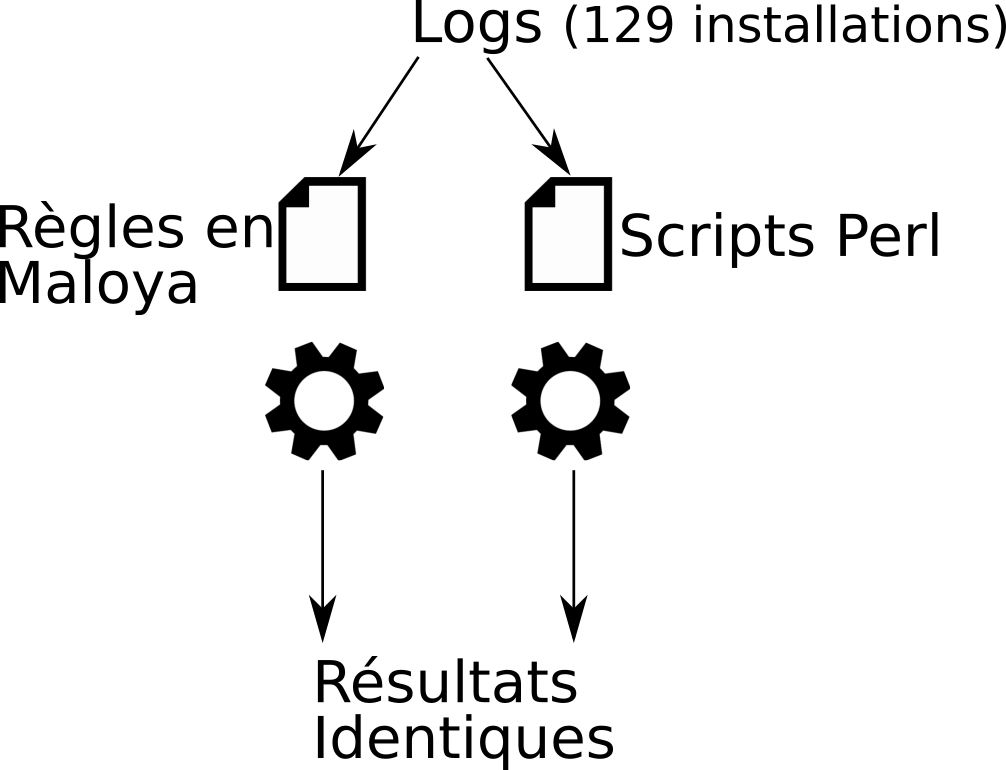
\includegraphics[scale=0.225]{perl.png}
\end{coloredbox}
}
\end{minipage}
\vfill
\end{frame}

% \begin{frame}{Synthèse}
%   \begin{itemize}
%   \item Approche unifiée de définition de services.
%   \item Règles manipulant des données de contextes à travers des évènement et des états.
%   \item Abstraction masquant la complexité du traitement d'évènements complexes.
%   \item Réactivité suffisante pour les besoins du domaine.
%   \end{itemize}
% % Unified approach to define services\\
% % Rules manipulating context data as state and event (cover domain concepts).\\
% % Abstraction hides event processing complexity (ease services expression).\\
% % Reactivity sufficient to cover domain requirements.\\
% \end{frame}

%\include{compiler}

\section*{Conclusion}
\begin{frame}{Conclusion~: couvrir les besoins des services sensibles au contexte}
\begin{minipage}{.5\linewidth}
Langage dédié~:
\begin{itemize}
\item Définition de services unifiée.
\item Expressivité couvre \\les objectifs de services.
\item Modèle d'infrastructure exprimé avec des services.
\end{itemize}
\end{minipage}
\hfill
\begin{minipage}{.45\linewidth}
    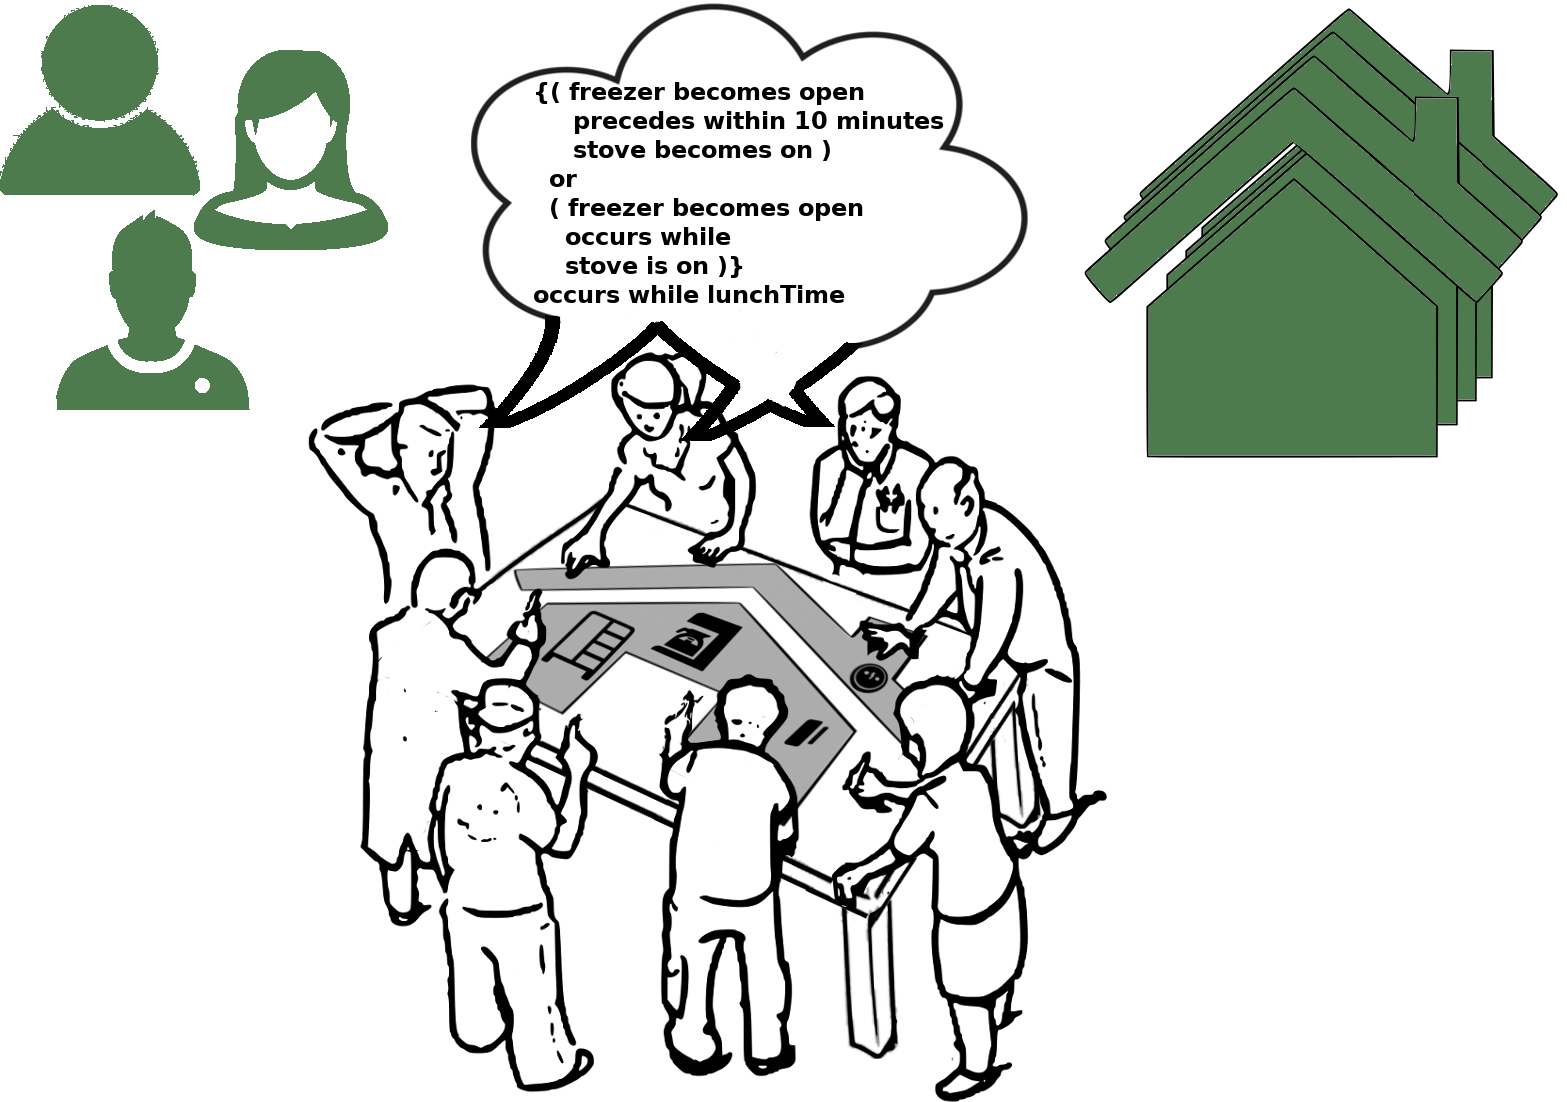
\includegraphics[scale=0.1]{axe_variation_final.png}
\end{minipage}
\vfill
Compilation masquant la complexité du traitement événementiel~:
\begin{itemize}
\item Services plus facile à exprimer et comprendre.
\end{itemize}

% Définition de services unifiée.
% \vfill
% Expressivité couvre les objectifs de services.
% \vfill
% Services plus facile à exprimer et comprendre.
% \vfill
% Modèle d'infrastructure exprimé avec des services.

% Unified approach to define services.\\
% Expessivity allow to cover objective of services.\\
% Model of infrastructure can be expressed as services.\\
% Services are easier to express than using Java.\\

\end{frame}

\begin{frame}{Perspectives}
\begin{minipage}{.5\linewidth}
Définition de services par les intervenants~:\\
\begin{itemize}
\item Étude ergonomique en cours \\(compréhension).
\item Langage graphique \\(programmation).
\end{itemize}
\end{minipage}
\hfill
\begin{minipage}{.45\linewidth}
\vspace*{3.11mm}
    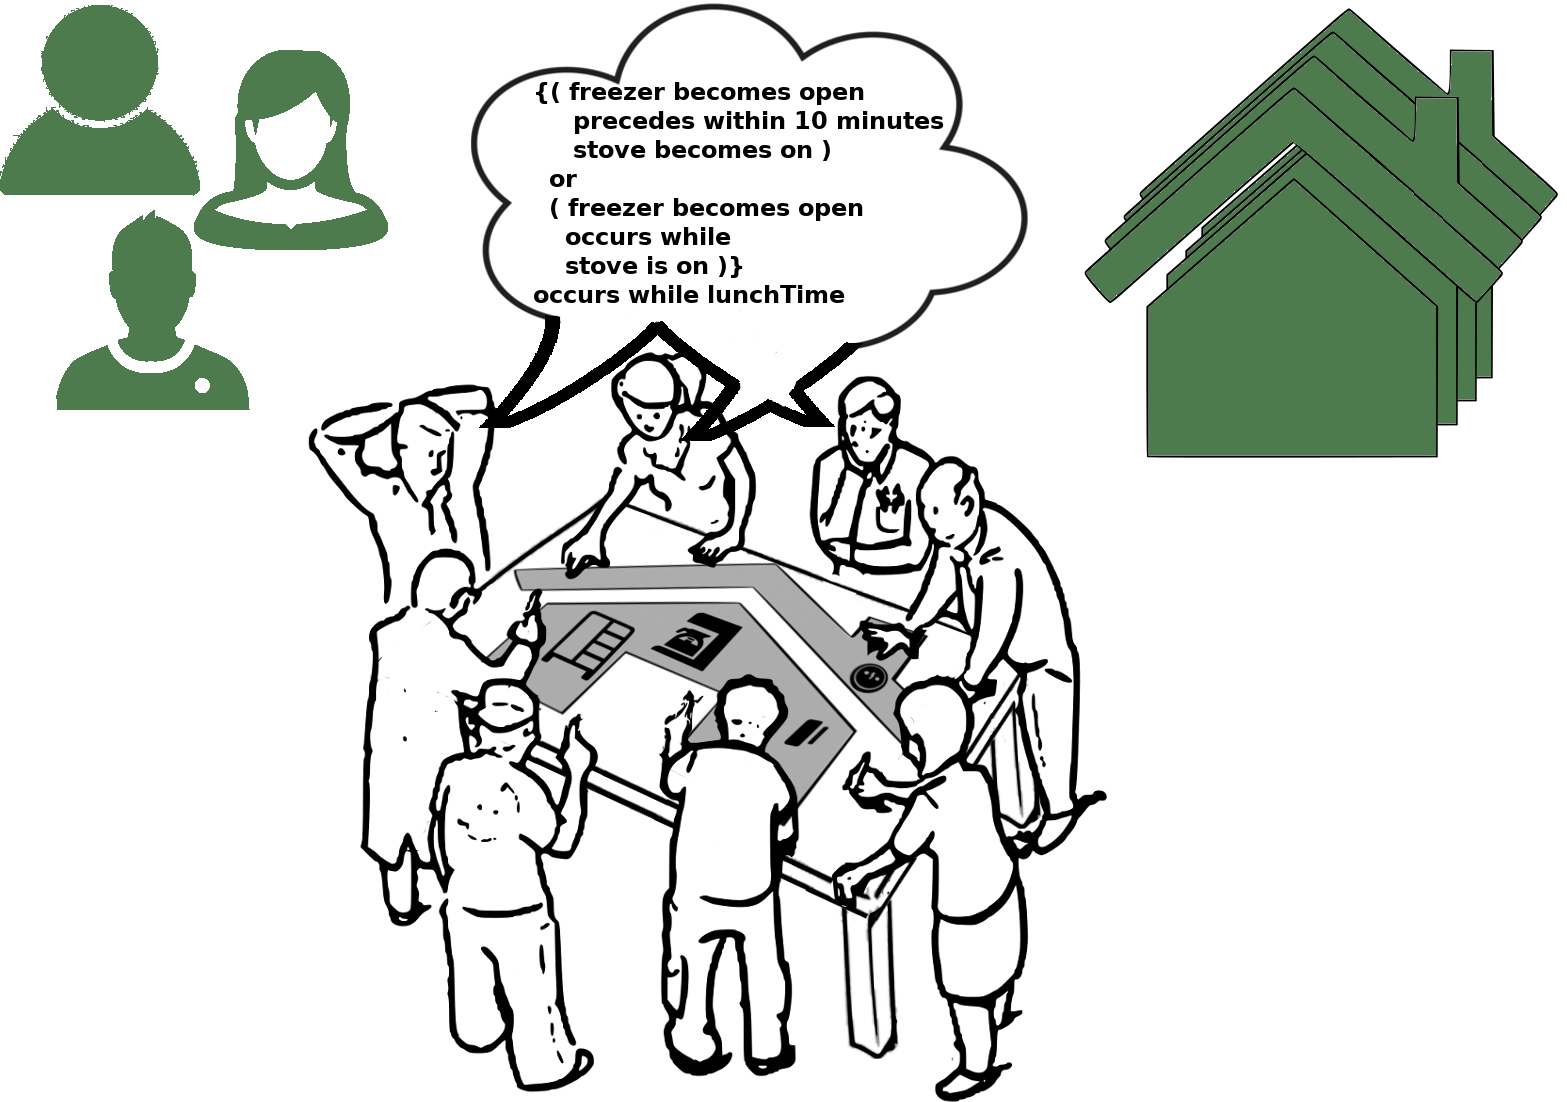
\includegraphics[scale=0.1]{axe_variation_final.png}
\end{minipage}
\vfill
Cibles de compilation~:\\
\begin{itemize}
\item Stream processing (Apache Spark, Flink).
%\item Couche graphique.
\end{itemize}
Évaluer le gain de l'éffort de développement.
% End-user service definition.\\
% Extend compilation targets.\\
\end{frame}

% \include{improv}
% \include{gener}
%\include{dsl}


% \begin{frame}[standout]
% Thank you!
% \end{frame}

\appendix
\begin{withoutheadline}
\begin{frame}%[allowframebreaks]
  \frametitle{Bibliographie}
  %\bibliographystyle{apalike}
   %\bibliographystyle{plain}
  %{\tiny\bibliography{bibliography.bib}}
\fullcite{carteron2016improving}
%{\tiny\printbibliography[notcategory=fullcited,heading=none]}
\end{frame}
%\include{backup}
\end{withoutheadline}

\end{document}